% Author: Joseph Rowell
% Version: 3.0
% This work is licensed under a Creative Commons Attribution 4.0 International License.
\documentclass[12pt, a4paper]{report}
\usepackage[a4paper, total={6.25in, 8.25in}]{geometry} %%%%%% CHECK MARGIN REQ. 8.25 in?
\input{Packages.tex}
\usepackage{multicol}
\hypersetup{pdftitle = {AI for Agriculture: Methane Emissions Gap-Filling, Forecasting, and Scenario Projection}, pdfauthor = {Nicholas Tobias}, pdfstartview=FitH, pdfkeywords = {methane flux, eddy covariance, gap-filling, time-series forecasting, tabular foundation models, scenario projection}, pdfpagemode = FullScreen, colorlinks, anchorcolor = black, citecolor = blue, urlcolor = blue, filecolor = green, linkcolor = blue, plainpages = false}
%%%%%%%%%%%%%%%%%%%%%%%%%%%%%%%%%%%%%%%%%%%%%%%%%%%%%%%%%%%%%%%%%%%%%%%
\pagestyle{fancy}
\rhead{}
\chead{}
\lhead{University College London}
\lfoot{\date{}}
\cfoot{}
\rfoot{\thepage}
% Top and Bottom Line Rules

\renewcommand{\headrulewidth}{0.4pt} %0.4pt
\renewcommand{\footrulewidth}{0.4pt}
\fancyheadoffset{8pt}
\fancyfootoffset{8pt}
% Line spacing
\renewcommand{\baselinestretch}{1.5} %1.5
\raggedbottom % let pages end short rather than stretching/overflowing into the footer

\input{Glossary}

\date{September 2026}

\title{AI for Agriculture: Methane Emissions Gap-Filling, Forecasting, and Scenario Projection}
\author{\\ \Large{Nicholas Tobias}
\\ Supervisors: 
\\ Paul Harris, Rothamsted Research
\\ Varun Varma, Rothamsted Research
\\ Andrea Karlova, UCL Computer Science
\\
\\ Faculty of Engineering
\\ Department of Computer Science
\\
\\ University College London
\\
A Project Report Presented in Partial Fulfillment of the Degree \\ \textit{MSc Artificial Intelligence for Sustainable Development}
\\
% \\Disclaimer:This report is submitted as part requirement for the MSc AI for Sustainable Development at University College London. It is substantially the result of my own work except where explicitly indicated in the text.The report may be freely copied and distributed provided the source is explicitly acknowledged.
% September 2026
}
%%%%%%%%%%%%%%%%%%%%%%%%%%%%%%%%%%%%%%%%%%%%%%%%%%%%%%%%%%%%%%%%%%%%%%%
\begin{document}
%Adjust logo positions here
% \AddToShipoutPicture*{\parbox[t][\paperheight][t]{\paperwidth}{%
%           \includegraphics[width=\paperwidth]{\BackgroundPicturea{Logos/ucl_long%_logo.png}{3in}{3in}}
%           }}
% \AddToShipoutPicture*{\centering\BackgroundPictureb{Logos/Bentham2011_065_c623d.jpg}{3in}{3.7in}}
\AddToShipoutPictureBG*{%
  \AtPageUpperLeft{%
    \raisebox{-\height}{%
      
\includegraphics[width=\paperwidth]{Logos/UCL page header.png}%
    }}
}
\AddToShipoutPicture*{%
      \parbox[t][\paperheight][t]{\paperwidth}{%
          
\includegraphics[width=1.2\paperwidth]{Logos/UCL page footer.png}
      }}
      

\thispagestyle{headings}
\maketitle
\FloatBarrier
\pagenumbering{roman}

\thispagestyle{empty}
\begin{abstract}
% % Methane (CH\textsubscript{4}) is a potent greenhouse gas with approximately
% % 28 times the global warming potential of CO\textsubscript{2} over 100 years,
% % and agriculture is a major anthropogenic source. Eddy Covariance measurements
% % capture ecosystem-scale emissions from managed grasslands, but these records
% % are often incomplete and dominated by episodic emission peaks, making methane
% % flux difficult to reconstruct and predict.

% Methane (CH\textsubscript{4}) is a potent greenhouse gas, with approximately 28
% times the global warming potential of CO\textsubscript{2} over 100 years. UK
% agriculture accounts for almost half (49\%) of national methane emissions 
% approximately 27 MtCO\textsubscript{2}e in 2024 with ruminant enteric fermentation
% forming the principal agricultural source. Eddy Covariance measurements provide
% ecosystem-scale observations from managed grasslands, but the resulting records are
% often incomplete and dominated by episodic emission peaks. Gap-filling supports the
% construction of continuous historical flux records, while forecasting provides a
% basis for anticipating future emissions and informing management decisions.

Methane (CH\textsubscript{4}) has approximately 28 times the 100-year global warming
potential of CO\textsubscript{2}. UK agriculture contributes almost half (49\%) of 
national methane emissions. Eddy 
Covariance (EC) provides ecosystem-scale observations of methane exchange over managed 
grasslands. 
% enabling data-driven modelling of environmental and management influences. 
However, EC records are often incomplete and characterised by episodic emission peaks. 
Gap-filling can reconstruct continuous historical flux records, while forecasting can 
anticipate future emissions and inform agricultural management.

This dissertation develops a three-stage machine-learning pipeline for
gap-filling, forecasting, and scenario projection using data from three
catchments at the North Wyke Farm Platform. Statistical, tree-based, neural,
and tabular pretrained foundation models were benchmarked using held-out and temporal
validation, supported by uncertainty quantification and permutation
importance. Future climate trajectories and emission scenarios were then combined with  
alternative farm management conditions to explore possible changes in methane flux.

% TabICLv2 achieved the strongest gap-filling performance, increasing combined 
% hourly $R^2$ from 0.055 for marginal distribution sampling to 0.515. TabPFN 
% led forecasting with MASE$=0.6908$, although performance deteriorated from 
% 0.524 on ordinary days to 3.285 during methane spikes. 

% The pretrained tabular models provided the strongest overall performance for 
% both gap-filling and forecasting. Among the models tested, traditional tree-based 
% models generally outperformed neural networks with the exception of tabular pretrained models. 

Overall performance follows a consistent pattern of tabular pretrained models performing best,
followed by tree-based models, and locally trained neural networks generally underperforming.
Nevertheless, sudden methane peaks remained difficult to anticipate for all models. 
Among the tested scenarios, livestock density produced the largest change in predicted annual 
CH\textsubscript{4} flux, followed by grazing duration, whereas varying fertiliser 
application rates produced little to no change in the modelled response.

Overall, pretrained foundation models for tabular data performed best across the predictive tasks,
while livestock-associated variables formed the strongest recurring influence
at the livestock-dominated catchments. However, severe target missingness,
emission spikes, and the absence of future ground truth limit 
the operational utility of these models.

\enlargethispage{\baselineskip}
\par\noindent
\keywords{methane flux -- eddy covariance -- time-series forecasting -- gap-filling}
% \vspace{-10mm} %To remove added white space after
\end{abstract}

% \thispagestyle{empty}
% \chapter*{Acknowledgements}

\thispagestyle{empty}
\chapter*{Declaration}
I, Nicholas Tobias, declare that this thesis has been composed by myself and that the work has not
been submitted for any other degree or professional qualification. I confirm that the work submitted
is my own, except where work that formed part of jointly authored publications has been included and
appropriately referenced. The report may be freely copied and distributed provided that the source is
explicitly acknowledged.

\vspace{1.5cm}

\noindent
\begin{minipage}[t]{0.46\textwidth}
  \parbox[b][1.2cm][b]{\linewidth}{%
    {\fontfamily{pzc}\selectfont\LARGE Nicholas Tobias}}
  \hrule
  \vspace{0.15cm}
  \textit{Signature}
\end{minipage}%
\hfill
\begin{minipage}[t]{0.46\textwidth}
  \parbox[b][1.2cm][b]{\linewidth}{27 August 2026}
  \hrule
  \vspace{0.15cm}
  \textit{Date}
\end{minipage}



\tableofcontents

\thispagestyle{plain}
\listoffigures
\listoftables
%\lstlistoflistings
% \listofalgorithms


%\begin{singlespace}
\chapter*{List of Abbreviations}
\begin{sortedlist} %sort alphabetically
  \sortitem{ACF:     Autocorrelation Function}
  \sortitem{AIC:     Akaike Information Criterion}
  \sortitem{ANN:     Artificial Neural Network}
  \sortitem{AR:      Autoregressive}
  \sortitem{Bi-LSTM: Bidirectional Long Short-Term Memory}
  \sortitem{CMIP6:   Coupled Model Intercomparison Project Phase 6}
  \sortitem{CQR:     Conformalized Quantile Regression}
  \sortitem{CV:      Cross-Validation}
  \sortitem{DL:      Deep Learning}
  \sortitem{DLinear: Decomposition-Linear Model}
  \sortitem{DOY:     Day Of Year}
  \sortitem{EC:      Eddy Covariance}
  \sortitem{FCH\textsubscript{4}:    Methane Flux}
  \sortitem{FCO\textsubscript{2}:    Carbon Dioxide Flux}
  \sortitem{GCM:     Global Climate Model}
  \sortitem{GPP:     Gross Primary Productivity}
  \sortitem{LightGBM: Light Gradient Boosting Machine}
  \sortitem{LSTM:    Long Short-Term Memory}
  \sortitem{LSU:     Livestock Unit}
  \sortitem{MAE:     Mean Absolute Error}
  \sortitem{MASE:    Mean Absolute Scaled Error}
  \sortitem{MDS:     Marginal Distribution Sampling}
  \sortitem{MET:     Meteorological Station}
  \sortitem{MICE:    Multivariate Imputation by Chained Equations}
  \sortitem{ML:      Machine Learning}
  \sortitem{MPIW:    Mean Prediction Interval Width}
  \sortitem{NWFP:    North Wyke Farm Platform}
  \sortitem{OLS:     Ordinary Least Squares}
  \sortitem{PACF:    Partial Autocorrelation Function}
  \sortitem{PCA:     Principal Component Analysis}
  \sortitem{PICP:    Prediction Interval Coverage Probability}
  \sortitem{PPFD:    Photosynthetic Photon Flux Density}
  \sortitem{QC:      Quality Control}
  \sortitem{QRF:     Quantile Regression Forest}
  \sortitem{RF:      Random Forest}
  \sortitem{RFm:     Random Forest (met-driven variant)}
  \sortitem{RMSE:    Root Mean Squared Error}
  \sortitem{SAITS:   Self-Attention-based Imputation for Time Series}
  \sortitem{SARIMAX: Seasonal AutoRegressive Integrated Moving Average with eXogenous regressors}
  \sortitem{SMS:     Soil Moisture Station}
  \sortitem{SSITC:   Steady-State and Integral Turbulence Characteristics}
  \sortitem{SSP:     Shared Socioeconomic Pathway}
  \sortitem{STL:     Seasonal-Trend decomposition using Loess}
  \sortitem{SVM:     Support Vector Machine}
  \sortitem{TabICLv2: Tabular In-Context Learning Version 2}
  \sortitem{TabPFN:  Tabular Prior-Data Fitted Network}
  \sortitem{TFT:     Temporal Fusion Transformer}
  \sortitem{TICA:    Time-lagged Independent Component Analysis}
  \sortitem{UMAP:    Uniform Manifold Approximation and Projection}
  \sortitem{UQ:      Uncertainty Quantification}
  \sortitem{VPD:     Vapour Pressure Deficit}
  \sortitem{WAPE:    Weighted Absolute Percentage Error}
  \sortitem{XGB/XGBoost: Extreme Gradient Boosting}
  \end{sortedlist}
% \end{singlespace}
\clearpage
\pagenumbering{arabic}
%%%%%%%%%%%%%%%%%%%%%%%%%%%%%%%%%%%%%%%%%%%%%%%%%%%%%%%%%%%%%%%%%%%%%%%%%%%%%%%%
\chapter{Introduction} \label{Chap1}

\section{Research Objective}

Methane (CH\textsubscript{4}) is a powerful greenhouse gas, with a global
warming potential approximately 28 times that of CO\textsubscript{2} over a
100-year horizon \cite{ipcc2021}. Agriculture is a major anthropogenic source,
with enteric fermentation accounting for a substantial proportion of the
sector's greenhouse gas emissions \cite{fao2023,eea2024}. However, emissions
from managed grasslands vary through time as livestock activity interacts with
soil, meteorological, and management conditions. Understanding this variability
therefore requires prediction of when ecosystem-scale emissions occur and how they 
respond to changes in farm management.

Eddy Covariance (EC) measurements provide a means of observing this integrated
ecosystem-scale signal rather than methane emitted by individual animals alone.
The North Wyke Farm Platform (NWFP) offers a rare record of half-hourly EC
CH\textsubscript{4} flux from managed beef-cattle grasslands, accompanied by
meteorological, soil, hydrological, and livestock-management data
\cite{hawkins2025,cardenas2022}. This creates an opportunity for
data-driven methane prediction, but also a difficult modelling problem: the
record contains extensive gaps, its inputs occur at different temporal
resolutions, and its target is highly variable and dominated by episodic
emission peaks.

Existing machine-learning research on EC CH\textsubscript{4} in a temperate grassland 
setting has primarily addressed gap-filling, in which missing observations are reconstructed within an
observed period \cite{irvin2021,zhu2023a}. Forecasting is a different task:
predictions must be generated sequentially using only information available at
the forecast origin. To the author's knowledge, no previous study has
benchmarked machine-learning forecasting of ecosystem-scale EC
CH\textsubscript{4} flux at a managed temperate grassland. Moreover, forecasting
alone cannot answer counterfactual questions about how emissions might change
under alternative livestock-management or climate conditions. This
``what-if'' capability is also an underdeveloped area of research in agricultural digital twins \cite{purcell2023state,fakeye2024}.

The objective of this dissertation is therefore to determine how effectively
machine-learning models can reconstruct, forecast, and project ecosystem-scale
CH\textsubscript{4} flux at NWFP. It develops a three-stage
pipeline for gap-filling the observed Eddy Covariance record, forecasting future
flux, and projecting modelled responses under varying management and
climate scenarios. Model benchmarking is accompanied by uncertainty
quantification and interpretability so that predictive performance, confidence,
and inferred emission drivers can be evaluated together.

\section{Project Aims and Goals}

\subsection*{Aims:}
Advance research in machine learning for CH\textsubscript{4} flux prediction at 
managed grassland, with a focus on gap-filling, forecasting, and scenario projection
under contrasting livestock-management conditions.

\subsection*{Goals:}
\begin{enumerate}
    \item Generation of a pipeline for gap-filling, forecasting, and scenario projection of CH\textsubscript{4} flux at NWFP.
    \item Benchmarking of multiple model families (from classical statistical baselines, tree ensembles, 
    deep sequence models, to recent tabular foundation models) for gap-filling and forecasting.
    \item Apply uncertainty quantification (quantile machine learning) and interpretability 
    methods (permutation importance) across gap-filling, forecasting, and scenario projection.
    \item Generation of future projection under differing livestock-management practices based on 
    inference of previously generated model and CMIP6 climate projections.
\end{enumerate}

\section{Project Overview and Contributions}

This dissertation contributes three benchmarked results to the field:

\begin{enumerate}
    \item \textbf{A gap-filling benchmark for EC CH\textsubscript{4} flux at a managed
    grassland} (Chapter~\ref{Chap4}), comparing established methods, published baseline
    replications, and newer tabular foundation model families, with uncertainty quantification
    attached. The best configuration reaches an hourly-resolution $R^2$ of 0.429 - 0.686 across all
    three towers, against a published ceiling of $R^2<0.1$ at hourly resolution for the same
    ecosystem and data type \cite{zhu2023a}.

    \item \textbf{A forecasting benchmark for EC CH\textsubscript{4} flux at a managed grassland}
    (Chapter~\ref{Chap5}), the first, to the author's knowledge, applied to this ecosystem--data
    combination at a managed temperate grassland, comparing statistical baselines, tree ensembles, and
    tabular foundation models under identical conditions, with calibrated uncertainty quantification and
    interpretability through permutation importance. The best configuration beats seasonal-mean baseline 
    by a wide margin (MASE$=$0.691), though a dedicated error evaluation shows that spike events remain 
    a challenge for all models tested.

    \item \textbf{Scenario projection under contrasting management and climate conditions for EC CH\textsubscript{4} flux}
    (Chapter~\ref{Chap6}): the forecasting architecture developed in this dissertation is extended
    to produce varying CH\textsubscript{4} projections under livestock and management practices for 
    2 distinct climate scenarios (SSP2-4.5 and SSP5-8.5), based on CMIP6 climate projections.
\end{enumerate}

\section{Report Overview}
The subsequent chapters are structured as follows:
\begin{itemize}
    \item Chapter~\ref{Chap2} (\nameref{Chap2}) reviews the literature establishing the gap that this dissertation 
    aims to address, as well as the North Wyke Farm Platform (NWFP).
    \item Chapter~\ref{Chap3} (\nameref{Chap3}) describes the NWFP dataset, exploratory data analysis, and
    processing required.
    \item Chapter~\ref{ChapModels} (\nameref{ChapModels}) outlines the methodology used for the project, including the 
    models, evaluation metrics, cross-validation procedure, uncertainty quantification and 
    interpretability.
    \item Chapter~\ref{Chap4} (\nameref{Chap4}) presents the results of the gap-filling benchmark; 
    \item Chapter~\ref{Chap5} (\nameref{Chap5}) presents the results of the forecasting benchmark; 
    \item Chapter~\ref{Chap6} (\nameref{Chap6}) presents the results of scenario projection.
    \item Chapter~\ref{Chap7} (\nameref{Chap7}) discusses the principal findings, their limitations and directions for future work before concluding the dissertation.    
    % \item Chapter~\ref{Chap8} (\nameref{Chap8}) concludes with an overview of the entire project.
\end{itemize}

%%%%%%%%%%%%%%%%%%%%%%%%%%%%%%%%%%%%%%%%%%%%%%%%%%%%%%%%%%%%%%%%%%%%%%%%%%%%%%%%
\chapter{Background and Related Work} \label{Chap2}

% ############################################################################
\section{North Wyke Farm Platform and Eddy Covariance Measurement}

% ############################################################################
\subsection{Experimental Design and Management Regimes}

The North Wyke Farm Platform (NWFP), operated by Rothamsted Research near
Okehampton in Devon, UK, is a farm-scale National Bioscience Research
Infrastructure established in 2010 to investigate the productivity and
environmental sustainability of temperate livestock and arable farming
systems. The platform covers approximately 63~ha and comprises three outdoor
experimental systems, known as the Red, Green, and Blue farmlets, each
covering approximately 21~ha. Each farmlet contains five hydrologically
isolated catchments, giving 15 catchments across the platform in total.
Catchments may comprise either a single field or multiple separately managed
fields. They are hydrologically isolated through the combined effects of local
topography, slowly permeable subsoils, and a 9.2-km network of French drains
that directs runoff towards instrumented flumes
\cite{hawkins2023design,hawkins2025}.

The three farmlets represent contrasting agricultural management systems. The Red farmlet operates 
as an arable system with crop rotations including wheat, oats, and field beans. The Green farmlet 
represents a conventional permanent-pasture system, supporting seasonal cattle and sheep grazing 
alongside silage production and inorganic fertiliser application. The Blue farmlet combines high-sugar 
perennial ryegrass with white clover, supporting outdoor livestock production while using biological 
nitrogen fixation to reduce reliance on inorganic nitrogen fertiliser. Together, the farmlets allow 
arable, permanent-pasture, and grass--clover livestock systems to be studied under the same wider 
environmental setting \cite{hawkins2023design,hawkins2023fieldevents}.

\begin{figure}[htbp]
    \centering
    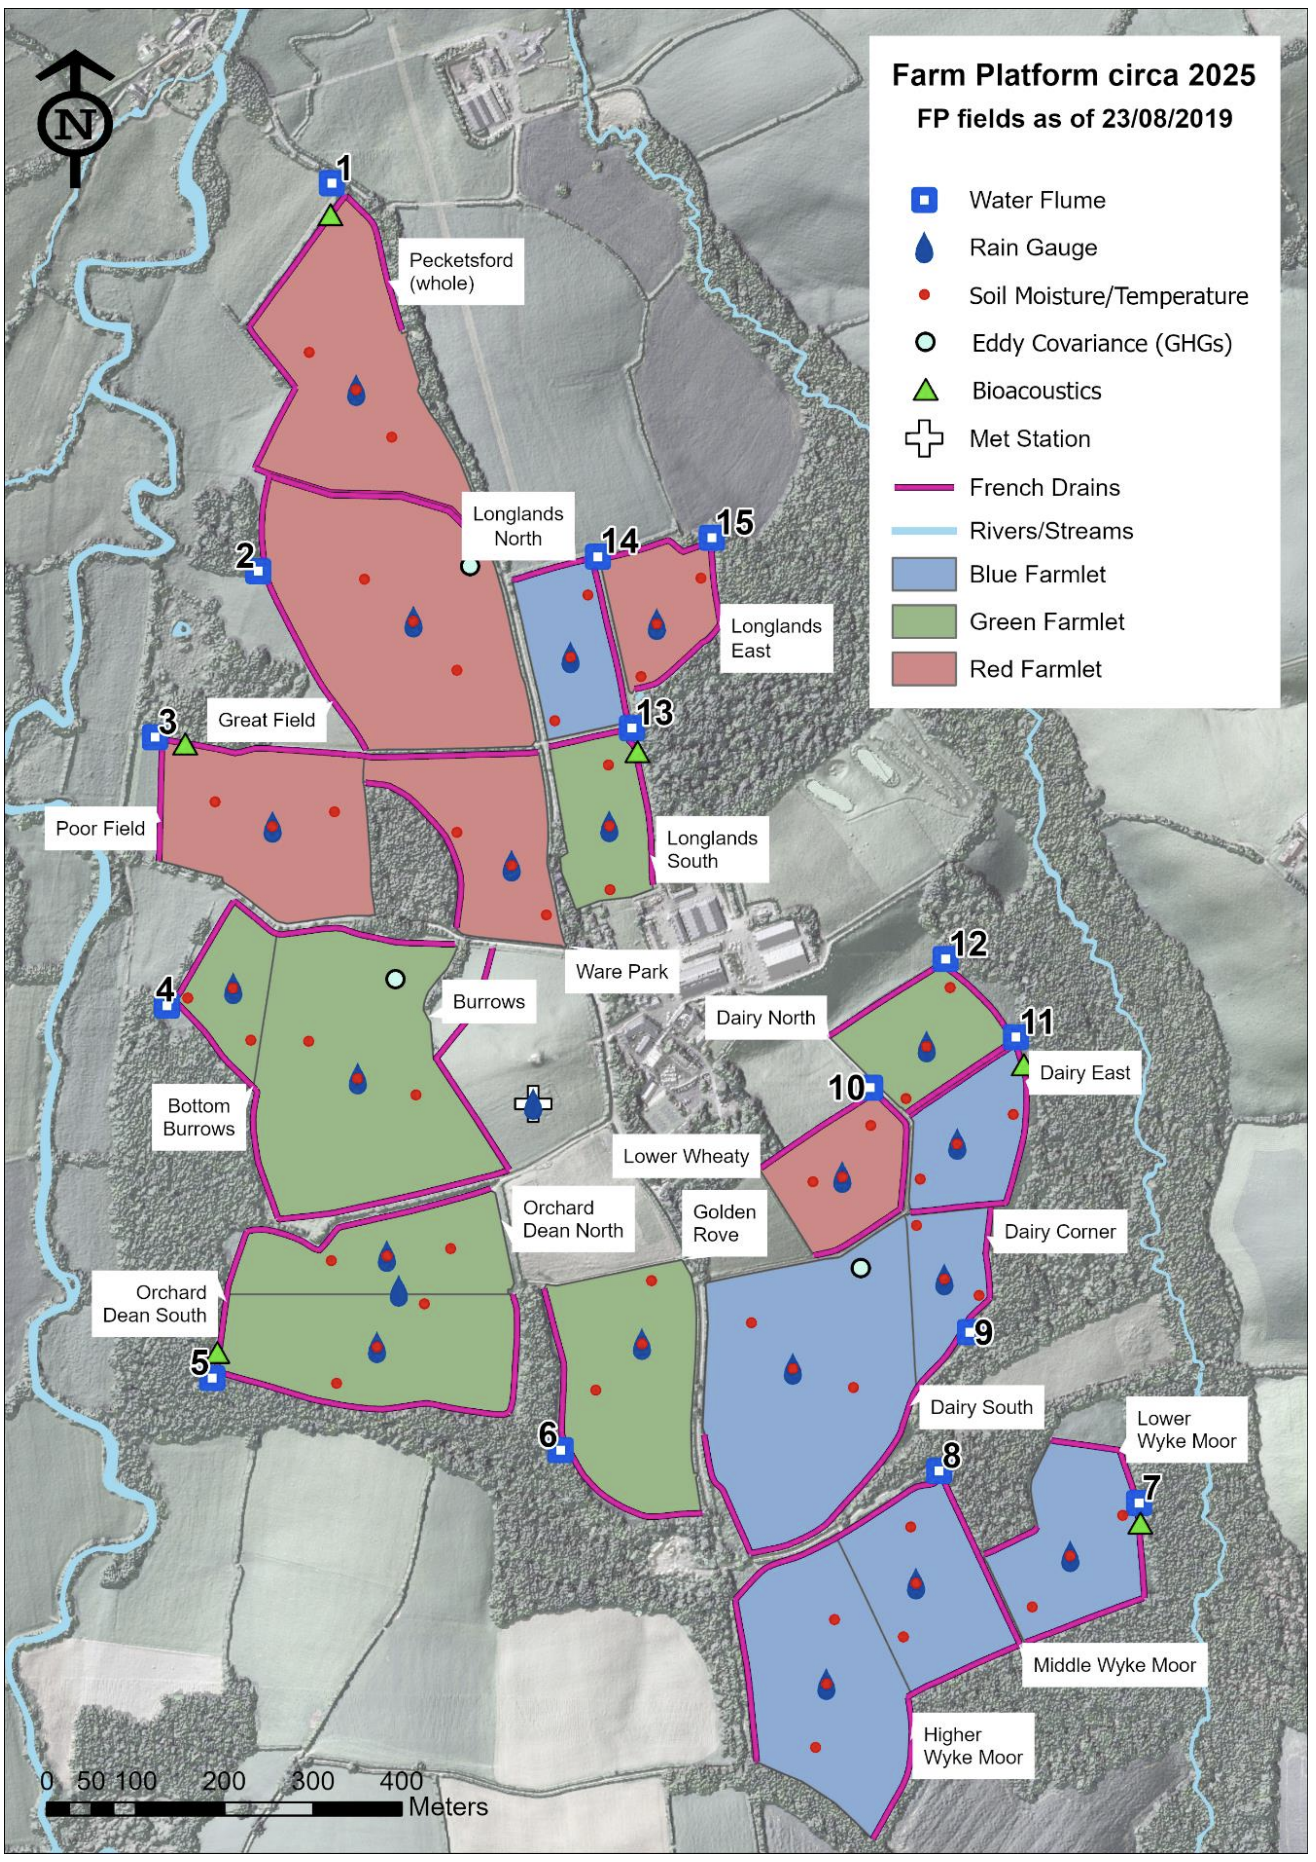
\includegraphics[
        width=0.82\textwidth,
        height=0.74\textheight,
        keepaspectratio
    ]{Figures/ch2_NWFP Map.png}
    \caption{Layout of the North Wyke Farm Platform circa 2025, showing the
    Red, Green, and Blue farmlets; The EC systems considered in this dissertation are
    situated in Great Field within Catchment~2, Burrows within Catchment~4,
    and Dairy South within Catchment~9. Cited from
    \cite{hawkins2023design}}
    \label{fig:nwfp-map}
\end{figure}

This dissertation examines measurements associated with three selected
catchments: Catchment~2 on the Red farmlet, Catchment~4 on the Green farmlet,
and Catchment~9 on the Blue farmlet, shown in
Figure~\ref{fig:nwfp-map}. These locations are denoted T2, T4, and T9
throughout the dissertation. The notation identifies the catchment containing
each EC site; it does not imply that NWFP comprises only three catchments.
Moreover, the three locations differ substantially in land use, vegetation,
livestock exposure, and measurement history. They should therefore be treated
as distinct modelling contexts rather than spatial replicates of a single
grassland treatment.

\begin{table}[htbp]
    \centering
    \small
    \caption{Characteristics of the NWFP catchments associated with the Eddy Covariance Towers.}
    \label{tab:nwfp-catchments}
    \begin{tabular}{
        @{}
        >{\raggedright\arraybackslash}p{0.07\textwidth}
        >{\raggedright\arraybackslash}p{0.19\textwidth}
        >{\raggedright\arraybackslash}p{0.35\textwidth}
        >{\raggedright\arraybackslash}p{0.30\textwidth}
        @{}
    }
        \toprule
        \textbf{Site} &
        \textbf{Location} &
        \textbf{Land use and management} &
        \textbf{Modelling significance} \\
        \midrule

        T2 &
        Catchment~2, Great Field, Red farmlet &
        Arable rotation including wheat, oats, and field beans. Great Field
        previously supported reseeded high-sugar perennial ryegrass, livestock
        grazing, and silage production. &
        Represents a pronounced grassland-to-arable transition rather than a
        continuously grazed pasture system. \\

        \addlinespace

        T4 &
        Catchment~4, Burrows, Green farmlet &
        Long-term permanent pasture managed through seasonal cattle and sheep
        grazing, silage production, inorganic fertiliser application, and the
        return of farmyard manure. &
        Represents the permanent-pasture system. Livestock presence within the
        EC footprint varies as animals rotate among fields. \\

        \addlinespace

        T9 &
        Catchment~9, Dairy South, Blue farmlet &
        High-sugar perennial ryegrass and white-clover pasture supporting
        cattle and sheep grazing and silage production, with biological nitrogen
        fixation reducing reliance on inorganic nitrogen fertiliser. &
        Represents the grass--clover livestock system, with temporally variable
        livestock presence and management activity. \\

        \bottomrule
    \end{tabular}
\end{table}

Together, T2, T4, and T9 represent three distinct combinations of land use,
vegetation, livestock exposure, and measurement availability. T2 captures a
grassland-to-arable transition, T4 represents long-term permanent pasture, and
T9 represents an established grass--clover livestock system. These differences
mean that observations from the three sites cannot be interpreted as spatial
replicates of a common management regime.

% ############################################################################
\subsection{Eddy Covariance Measurement and Flux Processing}

Eddy Covariance (EC) estimates the vertical exchange of a gas between the land
surface and atmosphere by combining rapid measurements of vertical wind velocity
with corresponding changes in gas concentration. In simplified form, the
turbulent flux of a gas \(c\) can be expressed as

\begin{equation}
    F_c = \overline{w'c'},
\end{equation}

where \(w'\) is the deviation of vertical wind velocity from its
averaging-period mean, \(c'\) is the corresponding deviation in gas
concentration, and the overbar denotes averaging through time. EC therefore
measures spatially integrated ecosystem exchange rather than emissions from an
individual source.

Each of the three EC systems identified in
Table~\ref{tab:nwfp-catchments} contains a Gill WindMaster Pro sonic anemometer
and an enclosed LI-7200RS analyser measuring carbon dioxide and water vapour.
Carbon-dioxide and water-vapour fluxes have been collected at all three systems
since January 2017. Two open-path LI-7700 analysers were subsequently deployed
for methane measurement from January 2018.

Because only two methane analysers were available, methane was not measured
continuously at all three locations. The analysers were initially installed at
T2 and T4 from January 2018 to June 2019. In July 2019, the analyser at T2 was
relocated to T9 following the conversion of the Red farmlet to arable
production. Consequently, T2 provides an earlier methane record from the Red
pasture system, T4 provides the most temporally consistent record, and T9
provides a later record from the Blue grass--clover system
\cite{olde2023ec}. These records are therefore neither continuous nor fully
contemporaneous.

Raw EC measurements are processed using EddyPro software, which calculates gas
fluxes and produces 30-minute averages recorded at the beginning and midpoint
of each hour. Timestamps are maintained in Coordinated Universal Time using the
analysers' GPS units. The resulting files follow the European Fluxes Database
format and retain quality flags, friction-velocity measurements, and footprint
information. Low-quality observations are not removed automatically and must
therefore be identified during data preparation \cite{olde2023ec}.

An EC observation represents a changing spatial footprint rather than a fixed
average of the field or catchment containing the system. The location and extent
of this footprint depend on wind direction, wind speed, atmospheric stability,
and measurement height, and may occasionally extend beyond the field boundary.
Recorded livestock presence at catchment level does not therefore guarantee that
the animals were inside the EC footprint at a particular timestamp. The
resulting FCH\textsubscript{4} measurement should be interpreted as integrated
methane exchange within this changing footprint.

This measurement scale also distinguishes EC from systems such as GreenFeed.
GreenFeed records methane released by an individual animal during discrete
visits, whereas EC integrates methane exchange associated with livestock,
manure, soil, vegetation, and other processes within its footprint
\cite{olde2023ec,demeofilho2023greenfeed}.

% ############################################################################
\subsection{EC Methane Gap-Filling and the Forecasting Gap}

EC records are rarely complete. Instrument maintenance, analyser servicing,
quality-control filtering, insufficient atmospheric turbulence, and periods in
which the estimated footprint falls outside the intended field can all remove
observations. At NWFP, these operational gaps coexist with the longer structural
absence created by relocating the methane analyser from T2 to T9. A continuous
historical FCH\textsubscript{4} series must therefore be constructed before flux
summaries and downstream forecasting models can be developed.

Zhu et al.\ provide the closest published same-site gap-filling comparison,
having evaluated MDS and machine-learning approaches using EC methane
measurements from the North Wyke managed pastures. All tested approaches
produced an OLS-regression \(R^2<0.10\) for FCH\textsubscript{4}: MDS achieved
approximately \(R^2=0.03\)--\(0.05\), while Random Forest performed relatively
better but remained below \(R^2=0.10\) \cite{zhu2023a}. These results establish
the difficulty of gap-filling methane flux at NWFP and provide the principal
published comparator for this dissertation. 

Evidence from other ecosystems generally supports the use of tree-based
methods. Irvin et al.\ found Random Forest and XGBoost to outperform neural and
linear models across 17 FLUXNET-CH4 wetland sites, although their uncertainty
estimates were systematically too narrow \cite{irvin2021}. Kim et al.\ similarly
reported strong Random Forest performance and found lagged environmental
variables particularly valuable for methane prediction \cite{kim2020}.
Nevertheless, these studies are dominated by wetlands and rice paddies rather
than managed livestock pasture. This motivates the same-site comparison of
established gap-filling methods, newer model families, and agricultural
management predictors undertaken in Chapter~\ref{Chap4}.

Importantly, these studies evaluate gap-filling rather than forecasting.
Gap-filling reconstructs missing observations within a historical record and
may use information from both before and after a gap. Forecasting instead
predicts beyond a defined forecast origin using only information available at
that point, with earlier predictions potentially becoming inputs during
recursive rollout. The published gap-filling results therefore establish a
relevant methodological baseline but do not demonstrate prospective predictive
skill. To the author's knowledge, no previous study has benchmarked multi-step
EC methane forecasting at a managed temperate grassland; this forms the second
modelling gap addressed by the dissertation.

% ############################################################################
\section{Advances in Tabular Machine Learning}
\label{sec:tabular-modelling}

Following temporal alignment and feature construction, the modelling tasks in
this dissertation take the form of supervised prediction over structured
tabular data. The candidate model families nevertheless differ substantially:
statistical models impose explicit temporal structure, tree ensembles learn
non-linear partitions from the study data, conventional deep-learning models
fit neural representations to the observed sequences, and tabular foundation
models transfer a prediction procedure learned through large-scale
pretraining. Two related questions therefore motivate the model roster used in
this dissertation: whether recent tabular foundation models transfer
effectively to EC methane data, and whether deep-learning methods outperform
established statistical and tree-based alternatives in this setting.

% ############################################################################
\subsection{Tabular Foundation Models}

Tabular foundation models are pretrained across many synthetic prediction tasks
and subsequently make predictions using labelled examples supplied as context.
The original TabPFN applied this approach to small classification problems,
while TabPFN v2 extended it to regression and larger tables
\cite{hollmann2023tabpfn,hollmann2025tabpfn}. TabPFN is not inherently a
time-series model, but Hoo et al.\ demonstrate that forecasting can be treated
as tabular regression by representing temporal position, seasonality, lags, and
other historical information as input features \cite{hoo2026tabpfnts}. This
formulation is directly relevant to the present dissertation, where EC methane
forecasting similarly uses calendar, environmental, management, and
autoregressive predictors.

TabICL was developed to extend in-context tabular learning to larger datasets
\cite{qu2025tabicl}. TabICLv2 subsequently introduced a redesigned
synthetic-data generator, more scalable attention, and revised pretraining
procedures, while supporting both regression and classification
\cite{qu2026tabiclv2}. Synthetic pretraining may be valuable at NWFP because
valid methane observations are limited, but general tabular benchmarks do not
establish performance under extensive missingness, non-stationarity, episodic
emission peaks, or recursive temporal extrapolation. The suitability of TabPFN
and TabICLv2 for EC methane modelling must therefore be determined through
task-specific evaluation.

% Tabular foundation models depart from conventional supervised learning by
% pretraining a neural model across many synthetic prediction tasks. The original
% TabPFN was trained to approximate Bayesian prediction over synthetically
% generated tabular datasets. At inference time, labelled training examples and
% unlabelled query examples are supplied together as context, allowing the model
% to generate predictions without conventional dataset-specific gradient-based
% training. The original implementation focused on small classification
% problems, while TabPFN v2 extended the approach to regression and larger
% tables \cite{hollmann2023tabpfn,hollmann2025tabpfn}. This combination of
% synthetic pretraining and in-context inference makes TabPFN potentially
% attractive where the available task-specific observations are limited.

% TabPFN is not inherently a time-series model. Hoo et al.\ address this by
% formulating forecasting as tabular regression: temporal position, seasonality,
% lags, and other historical information are represented as input features before
% inference with the pretrained TabPFN v2 model. Their TabPFN-TS approach
% therefore obtains forecasting capability without dedicated time-series
% pretraining \cite{hoo2026tabpfnts}. This formulation is directly relevant to
% the present dissertation, where EC methane forecasting is similarly represented
% using calendar, environmental, management, and autoregressive features.

% TabICL extends tabular in-context learning to larger datasets through an
% architecture designed to process features and observations more efficiently
% than earlier TabPFN implementations \cite{qu2025tabicl}. TabICLv2 subsequently
% extends this approach through a redesigned synthetic-data generator, more
% scalable attention, and revised pretraining procedures, while supporting both
% regression and classification \cite{qu2026tabiclv2}. Its relevance to this
% dissertation lies in the possibility that knowledge acquired during synthetic
% pretraining may compensate for the limited number of valid methane
% observations available at NWFP.

% Strong performance on general tabular benchmarks does not, however, guarantee
% successful transfer to EC methane modelling. NWFP combines extensive target
% missingness, heterogeneous environmental and management predictors,
% non-stationary land-management conditions, and a highly variable target
% containing episodic emission peaks. Forecasting also introduces temporal
% extrapolation and recursive error propagation that are absent from ordinary
% independent tabular regression. TabPFN and TabICLv2 must therefore be evaluated
% under the same task-specific temporal protocol as the other model families
% rather than assumed to be superior on the basis of their published benchmarks.

% ############################################################################
\subsection{Deep Learning versus Traditional Machine Learning}

Large tabular benchmarks do not establish universal superiority of deep
learning. Grinsztajn et al.\ compared tree ensembles and neural architectures
across 45 medium-sized datasets and found tree-based models to remain
state-of-the-art, attributing this partly to their robustness to uninformative
features and irregular response functions \cite{grinsztajn2022}. McElfresh
et al.\ reached a more conditional conclusion from 19 algorithms and 176
datasets: neural and boosted-tree performance was often similar, modest
boosted-tree tuning could matter more than model-family choice, and relative
performance depended strongly on dataset characteristics
\cite{mcelfresh2023}. This pattern is consistent with EC methane studies, in
which Random Forest and XGBoost have generally provided stronger baselines than
conventional neural alternatives \cite{irvin2021,kim2020,zhu2023a}. These
findings justify retaining tree ensembles as serious comparators without
assuming that they must remain superior when richer predictors or pretrained
models are introduced.

A comparable debate exists in time-series forecasting. Zeng et al.\ found that
simple one-layer linear models outperformed several Transformer architectures
across nine long-term forecasting datasets \cite{zeng2023}. This does not imply
that complex architectures are universally ineffective, but demonstrates that
architectural sophistication cannot itself be treated as evidence of predictive
skill. Tabular foundation models further complicate the comparison: TabPFN and
TabICLv2 are neural models, but their capabilities are largely acquired through
pretraining rather than learned exclusively from the study dataset. The
relevant empirical comparison is therefore among statistical baselines, tree
ensembles, locally trained deep-learning models, and pretrained tabular
foundation models under identical evaluation conditions.

% ############################################################################
\section{Synthesis and Gap Statement}

Existing research demonstrates that machine learning can reconstruct missing
EC methane observations, but the closest North Wyke comparison reports weak
predictive performance, and the wider evidence is dominated by wetlands and
rice paddies, not grassland farming. Moreover, these studies evaluate gap-filling 
within historical records rather than multi-step forecasting beyond a defined 
forecast origin. To the author's knowledge, no previous study has benchmarked 
methane flux forecasting at a managed temperate grassland.

Recent TabPFN and TabICL models have also not been evaluated for this
combination of ecosystem, measurement type, and prediction tasks. It therefore
remains unknown whether synthetic pretraining provides an advantage over
established statistical, tree-based, and conventional deep-learning approaches
under severe target missingness and temporal extrapolation. This dissertation
addresses these gaps by comparing the model families under common,
leakage-safe gap-filling and forecasting protocols, accompanied by uncertainty
quantification and interpretability. The resulting forecasting architecture is
then applied to bounded scenario projection under contrasting management and
climate conditions.

% Existing evidence does not establish a universally superior model family for
% structured environmental prediction. Large tabular benchmarks show that tree
% ensembles remain highly competitive, particularly for medium-sized and
% irregular datasets, but also demonstrate that the relative performance of
% neural and tree-based models depends on dataset characteristics and tuning
% \cite{grinsztajn2022,mcelfresh2023}. Meanwhile, the recent TabPFN and TabICL
% families have not been evaluated for EC methane gap-filling and multi-step
% forecasting at a managed temperate grassland. Whether synthetic pretraining
% offers an advantage under severe missingness, temporal extrapolation, and
% episodic methane behaviour therefore remains unresolved and presents an 
% opportunity for investigation within this dissertation.

%%%%%%%%%%%%%%%%%%%%%%%%%%%%%%%%%%%%%%%%%%%%%%%%%%%%%%%%%%%%%%%%%%%%%%%%%%%%%%%%
\chapter{Data} \label{Chap3}

\section{Dataset Overview}

The analytical dataset draws on five NWFP data sources: the site-wide meteorological station,
catchment soil moisture stations, eddy-covariance greenhouse-gas measurements, livestock-location
records, and field-event records. The greenhouse-gas source used here is the tower-based EC dataset.
A separate GreenFeed dataset measures emissions from individual animals but is excluded because it does
not represent the same tower-scale ecosystem exchange measured by EC. Table~\ref{tab:ch3_source_inventory}
summarises these sources, while detailed dictionaries describing downloaded raw variables and
project-derived variables are provided in Appendix~\ref{app:data-dictionary}.

{
\scriptsize
\setlength{\tabcolsep}{2pt}
\renewcommand{\arraystretch}{1.16}
\setlength\LTleft{0pt}
\setlength\LTright{0pt}
% \begin{longtable}{@{}p{0.22\textwidth}p{0.28\textwidth}p{\dimexpr0.50\textwidth-4\tabcolsep\relax}@{}}
\begin{longtable}{
@{}
>{\raggedright\arraybackslash}p{0.22\textwidth}
>{\raggedright\arraybackslash}p{0.28\textwidth}
>{\raggedright\arraybackslash}p{\dimexpr0.50\textwidth-4\tabcolsep\relax}
@{}
}
\caption{NWFP datasets used to construct the analytical dataset. Dataset scope follows the NWFP Data Guide and 
platform design guide \cite{hawkins2025,hawkins2023design}}
\label{tab:ch3_source_inventory}\\
\toprule
NWFP dataset & Availability and resolution & Contents \\
\midrule
\endfirsthead
\multicolumn{3}{l}{\tablename\ \thetable\ -- continued}\\
\toprule
NWFP dataset & Availability and resolution & Contents \\
\midrule
\endhead
\midrule
\multicolumn{3}{r}{Continued on next page}\\
\endfoot
\bottomrule
\endlastfoot
MET Station \cite{hawkins2023met} & 
31/10/2011--2 Mar 2026; 15 min & 
Site-level wind speed, air temperature, wind direction, relative humidity, solar radiation and precipitation \\

Soil Moisture Stations (SMS) \cite{hawkins2023sms} & 
31/10/2011--4 Mar 2024; 15 min & 
Catchment-level precipitation, soil moisture at 10 cm and soil temperature at 15 cm \\

Eddy Covariance Greenhouse Gas \cite{olde2023ec} & 
1/1/2017--1/1/2024; 30 min & 
Tower-level FCH\textsubscript{4}, FCO\textsubscript{2}, SSITC (quality) flags and associated EC biometeorological 
and turbulence variables, including VPD, PPFD, RN, USTAR and SHF \\

Livestock \cite{hawkins2025} & 
21/3/2011--21/4/2026; daily & 
Catchment-level daily location counts for livestock and weight \\

Field Events \cite{hawkins2023fieldevents} & 
5/1/2011--13/11/2025; event based, sparse & 
Field-level farm operations, grazing practices, silage, fertiliser additions \\
\end{longtable}
}

% Following time alignment and hourly aggregation, the consolidated table contained
% 70,153 hourly timestamps and 449 measurement variables. A modelling dataset with 30 
% variables for each tower from 2017 to 2025 is later constructed, 
% with valid coverage for EC modelling from 2017 to 1 January 2024. However, valid
% FCH\textsubscript{4} coverage within that window is not uniform across towers, 
% as will be discussed in the next section.

Following time alignment and hourly aggregation, the consolidated table
contained 70,153 hourly timestamps and 449 measurement variables. The hourly
gap-filling frame later uses 30 predictors per tower, while forecasting uses
the separate daily predictor frame described in Chapter~\ref{Chap5}. EC target
analysis is restricted to the period from 1 January 2017 to 1 January 2024.

% ############################################################################
\section{Exploratory Data Analysis and Data Preparation}
% ############################################################################
\subsection{Methane Target Availability}

Target availability was assessed over the common 61,344-hour EC analysis window from 1 January
2017 to 1 January 2024. Raw missingness indicates whether an hourly FCH\textsubscript{4} value is
present in the consolidated data. The modelling target is stricter: an observation is usable only
when its SSITC quality class is 0 or 1 and its flux lies within the project plausibility range of
$[-500,3000]$ nmol m$^{-2}$ s$^{-1}$. Table~\ref{tab:ch3_fch4_missingness} distinguishes these two
stages, while Figure~\ref{fig:ch3_fch4_availability} shows both the temporal behaviour of the usable
target and its annual completeness.

\begin{table}[htbp]
\centering
\small
\caption{Availability of hourly FCH\textsubscript{4} observations over the common 2017--2023 EC
analysis window. QC-valid observations pass the SSITC and plausibility filters used to construct the
modelling target.}
\label{tab:ch3_fch4_missingness}
\begin{tabular*}{\textwidth}{@{\extracolsep{\fill}}lrrrr@{}}
\toprule
Tower & Raw observed (h) & Raw missing (\%) & QC-valid (h) & Unavailable after QC (\%) \\
\midrule
T2 & 8,099 & 86.8 & 4,890 & 92.0 \\
T4 & 30,485 & 50.3 & 19,469 & 68.3 \\
T9 & 17,509 & 71.5 & 11,235 & 81.7 \\
\bottomrule
\end{tabular*}
\end{table}

\begin{figure}[htbp]
\centering
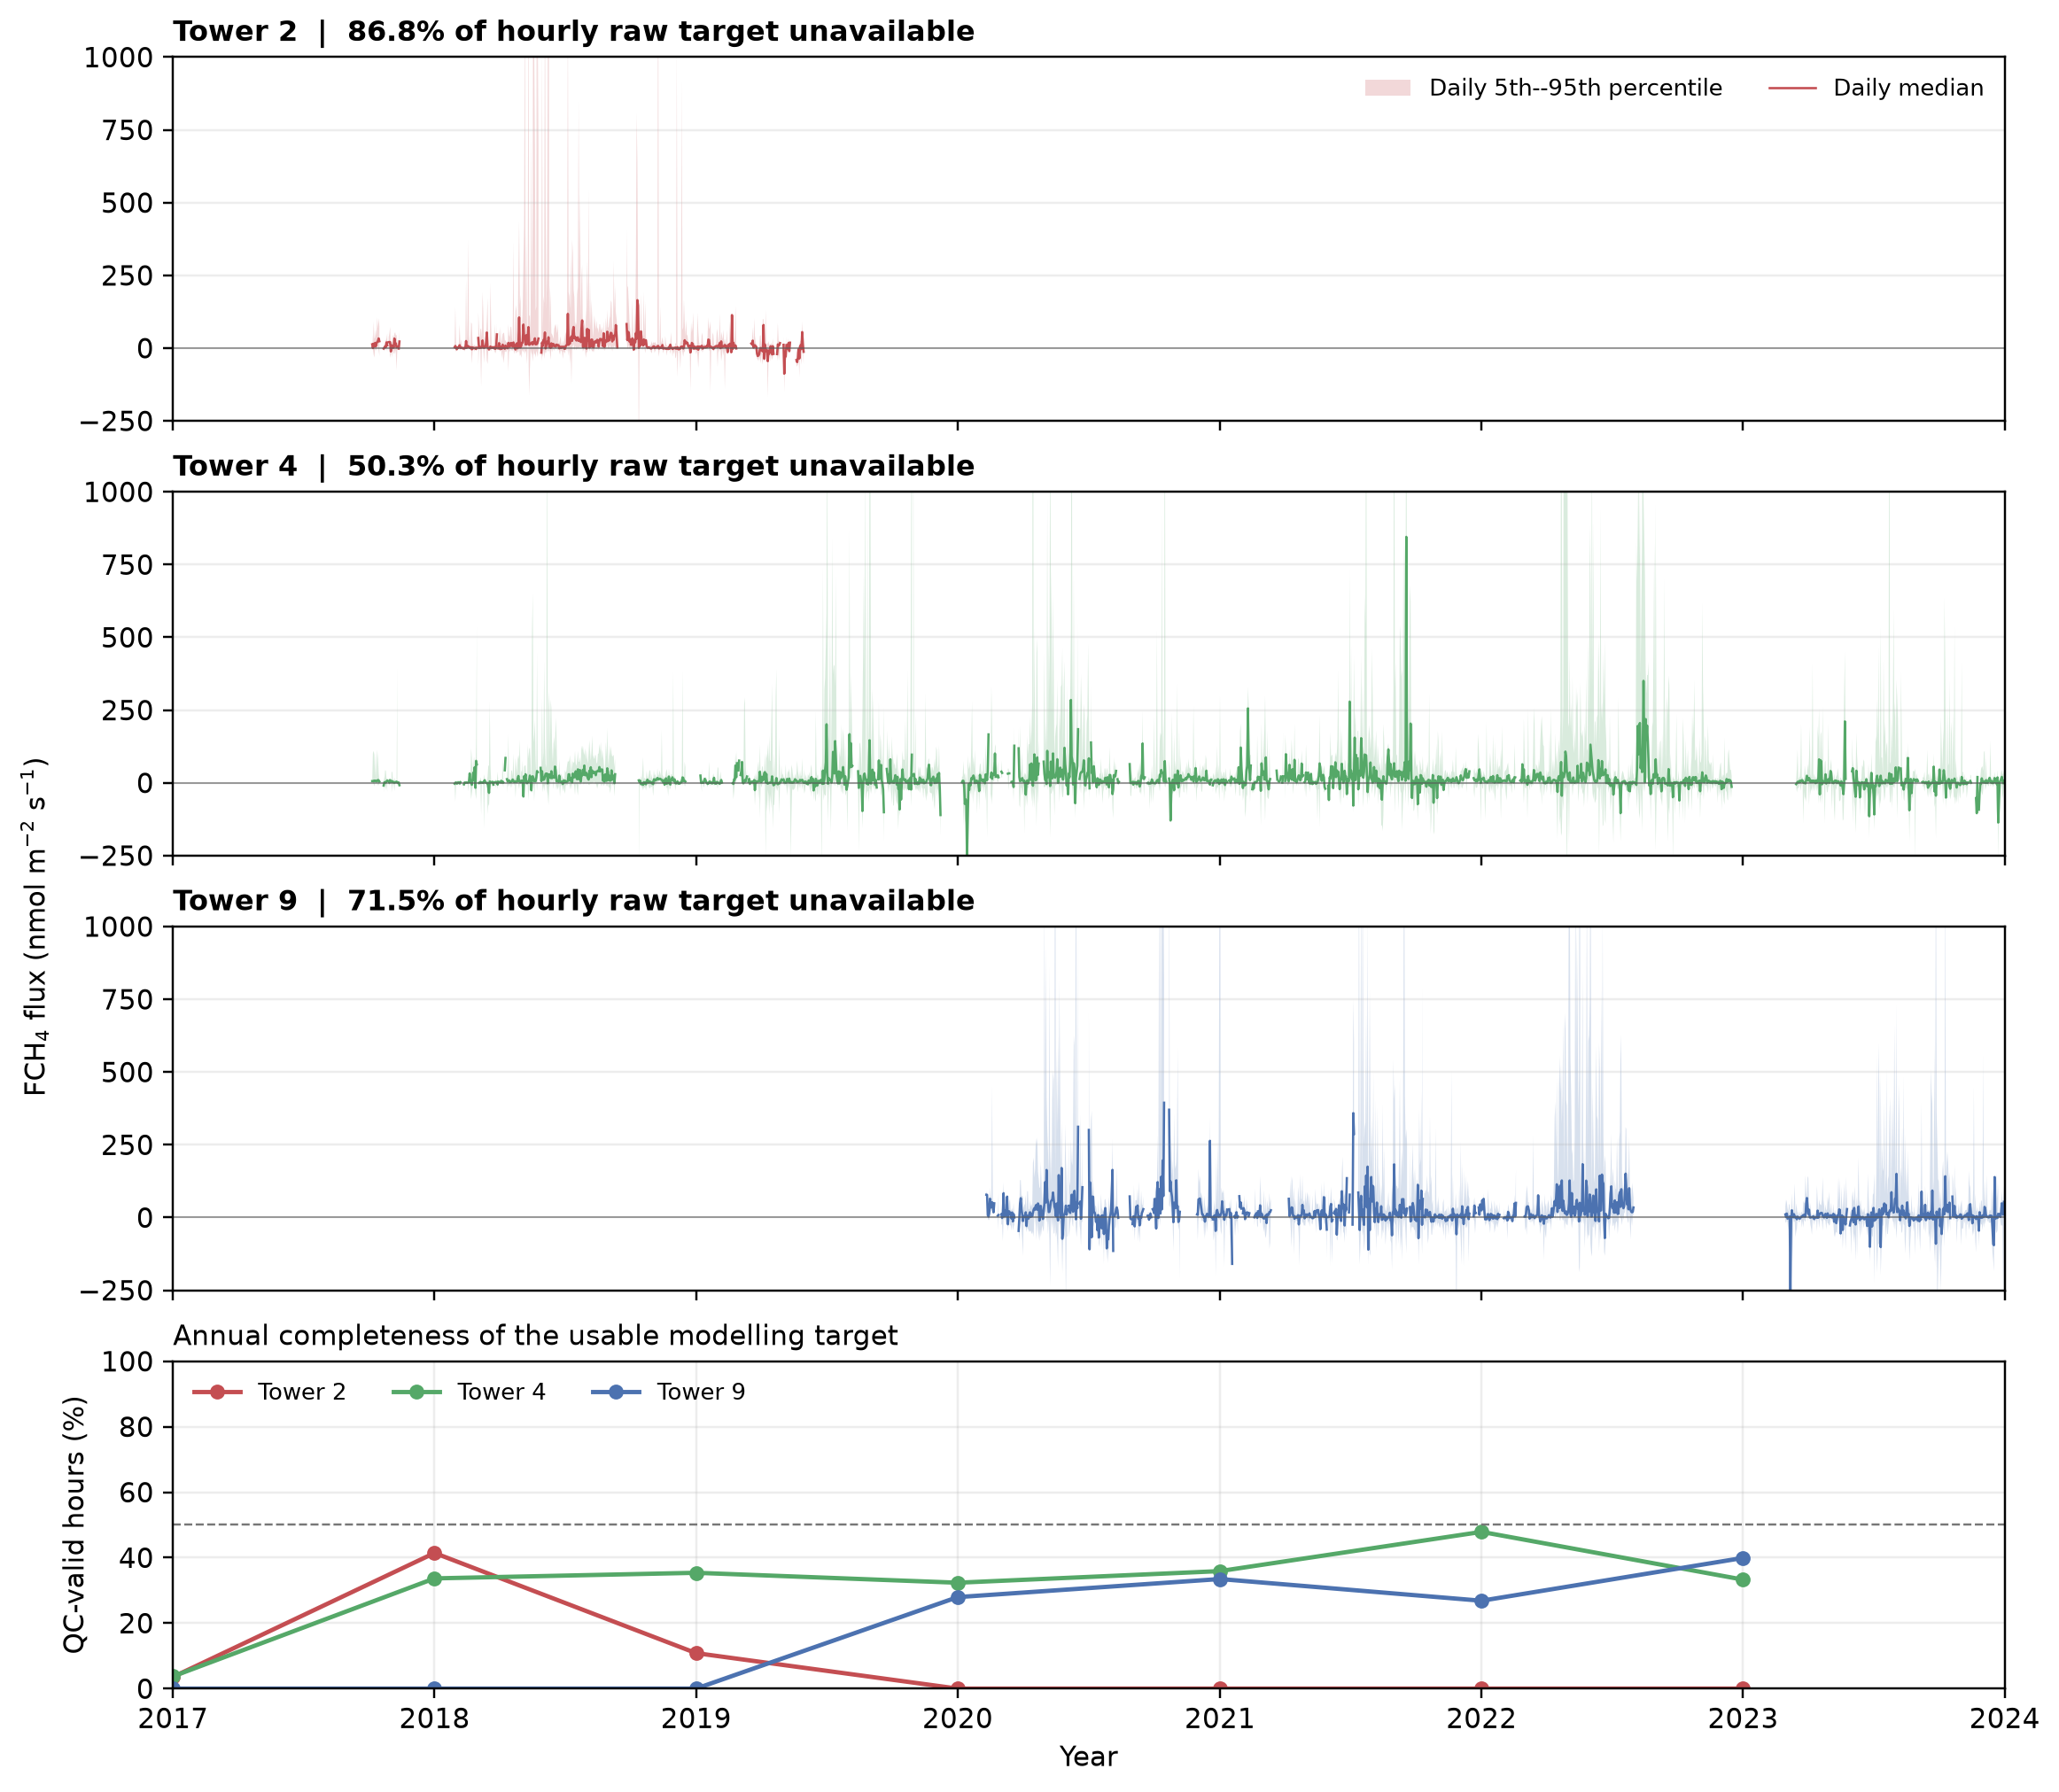
\includegraphics[width=\textwidth]{Figures/ch3_fch4_three_tower_availability.png}
\caption{
    Daily median FCH\textsubscript{4} flux (line) and 5th--95th percentile range (shaded) at towers T2, 
    T4, and T9, with hourly raw-data unavailability noted per panel. Bottom panel: annual 
    completeness of the QC-valid modelling target. Note that y-axis has been limited to $[-250,1000]$ 
    nmol m$^{-2}$ s$^{-1}$ for readability.
}
\label{fig:ch3_fch4_availability}
\end{figure}


Methane-target coverage is limited across all towers, with 92.0\% of common-window hours unavailable at T2, 
compared with 68.3\% at T4 and 81.7\% at T9. Missingness is temporally structured: T2 observations are 
concentrated in 2017--2019, after which its methane analyser was relocated to T9 following the Red 
farmlet's conversion to arable production \cite{olde2023ec}. T2 results should be interpreted cautiously due to its smaller, temporally 
narrower sample.

\FloatBarrier

% ############################################################################
\subsection{Quality Control and Environmental Variable Gap-Filling}
\label{sec:ch3_environmental_preparation}

Quality screening was applied before reconstruction so that rejected observations could not act as
anchors for filling. Hourly FCH\textsubscript{4} and FCO\textsubscript{2} observations were retained
only when their SSITC class was 0 or 1; values outside $[-500,3000]$~nmol
CH\textsubscript{4}~m$^{-2}$~s$^{-1}$ and $[-100,100]$~$\mu$mol
CO\textsubscript{2}~m$^{-2}$~s$^{-1}$, respectively, were set to missing. The effect on the methane
target is reported in Table~\ref{tab:ch3_fch4_missingness}. Before environmental-driver filling,
friction velocity was restricted to $[0,3]$~m~s$^{-1}$ and vapour-pressure deficit to $[0,15]$ on
the stored numerical scale because both fields contained extreme values. A separate low-turbulence
flag was retained as a diagnostic rather than used to reject FCH\textsubscript{4}, since such
filtering is not assumed to be a generally valid methane quality criterion.

Environmental-driver preparation combined two related procedures. The auxiliary-data calibration
workflow, detailed in Algorithm~\ref{alg:auxiliary-driver-gapfill} in
Appendix~\ref{app:data-dictionary}, was adapted from the North Wyke Farm Platform EC processing
report \cite{nwfp2022ecqc}. The subsequent temporal filling hierarchy was
implemented in Python and informed by the interpolation and mean-diurnal-course principles provided
by \texttt{REddyProc} \cite{wutzler2018reddyproc}; the R package itself was not invoked. The active
data path used the central MET station for shortwave radiation, air temperature and wind speed, the
corresponding catchment SMS for precipitation and soil conditions, and EC records for VPD, PPFD, net
radiation, friction velocity and soil heat flux.

Following source selection and plausibility screening, internal gaps were linearly interpolated for
up to 288 hours for air temperature, VPD, wind speed, soil moisture and soil temperature, and for up
to two hours for the remaining drivers. Unresolved gaps were filled from the mean diurnal course at
the same hour of day, first within a centred seven-day window and then, where necessary, within 14-,
28- and 60-day windows. Remaining gaps received the corresponding hour-of-day median and, only when
that was unavailable, the series-wide median. Accepted observations were preserved throughout the
temporal filling sequence. The resulting drivers are numerically complete while retaining local
diurnal structure where nearby observations exist; values produced during longer sensor blackouts
remain reconstructions rather than new measurements. This preprocessing was applied only to supporting 
model inputs; observed FCH\textsubscript{4} values were not imputed.

\begin{table}[htbp]
\centering
\small
\caption{
    Prior availability and synthetic-gap reconstruction accuracy of environmental drivers.
    Gap-CV $R^2$ is the mean across towers of the tower-level median over five gap-duration 
    (1h, 4h, 32h, 288h, mixed) scenarios. Each scenario masks 25\% of eligible observations 
    across two repetitions for evaluation. The auxiliary-data calibration component is detailed in
    Algorithm~\ref{alg:auxiliary-driver-gapfill} in Appendix~\ref{app:data-dictionary}.
}
\label{tab:ch3_environmental_gapfill}
\begin{tabular*}{\textwidth}{@{\extracolsep{\fill}}lrrrrr@{}}
\toprule
& \multicolumn{3}{c}{Available input (\%)} & \multicolumn{1}{c}{After filling (\%)}
& \multicolumn{1}{c}{Gap-CV $R^2$} \\
\cmidrule(lr){2-4}\cmidrule(lr){5-5}\cmidrule(l){6-6}
Driver & T2 & T4 & T9 & All towers & Mean across towers \\
\midrule
Shortwave radiation & 98.8 & 98.8 & 98.8 & 100.0 & 0.685 \\
Air temperature & 98.8 & 98.8 & 98.8 & 100.0 & 0.692 \\
Vapour-pressure deficit & 61.8 & 75.4 & 73.2 & 100.0 & 0.471 \\
Photosynthetic photon flux & 61.1 & 86.2 & 81.8 & 100.0 & 0.695 \\
Net radiation & 60.2 & 86.2 & 81.8 & 100.0 & 0.738 \\
Wind speed & 93.6 & 93.6 & 93.6 & 100.0 & 0.482 \\
Friction velocity & 81.2 & 88.2 & 84.4 & 100.0 & 0.000 \\
Soil heat flux & 43.3 & 86.2 & 81.8 & 100.0 & 0.532 \\
Precipitation & 83.1 & 85.7 & 62.5 & 100.0 & 0.012 \\
Soil moisture & 81.1 & 64.6 & 75.5 & 100.0 & 0.997 \\
Soil temperature & 83.7 & 65.6 & 78.9 & 100.0 & 0.993 \\
FCO\textsubscript{2} & 50.5 & 64.2 & 58.5 & 100.0 & 0.745 \\
\bottomrule
\end{tabular*}
\end{table}

Mean driver availability before reconstruction was 77.0\% at T2, 84.5\% at T4, and 82.8\% at T9. 
The staged procedure achieved 100\% numerical coverage across all 33 tower--driver series, but 
reconstruction accuracy varied considerably. Gap-CV performance was strongest for soil moisture and 
temperature, while precipitation and friction velocity showed limited skill. Thus, complete coverage 
does not imply equally reliable reconstruction across drivers. Their downstream contributions are 
evaluated in Chapter~\ref{Chap4}.

% ############################################################################
\subsection{Temporal Analysis and Dimensionality Reduction}

ACF and PACF were used to examine temporal dependence in the QC-valid
observed FCH\textsubscript{4} series without reconstructing long target
gaps. Weekly STL decomposition was also applied to the longest
sufficiently complete daily segment at each tower. Full diagnostics are
provided in Appendix Figures~\ref{fig:appendix_ch3_acf_pacf} and
\ref{fig:appendix_ch3_stl}.

Pairwise associations with the target were calculated from the same 30-predictor frame used in
the gap-filling experiments. Tower indicators were excluded because they are constant within each
tower, and correlations were calculated only where observed FCH\textsubscript{4} passed the target
quality and plausibility filters; gap-filled FCH\textsubscript{4} values were not used. Spearman's
rank correlation was selected because the target is highly skewed and spike-dominated, making a
rank-based measure more representative of monotonic association than Pearson correlation. The
calculation was performed separately for each tower using pairwise-complete observations.
For a concise comparison, Figure~\ref{fig:ch3_target_correlations} takes the five largest absolute
correlations within each tower and displays their union, while retaining all three tower coefficients
for every selected predictor. The complete 30-predictor matrix is provided in
Appendix Figure~\ref{fig:appendix_target_correlations_full}.

\begin{figure}[htbp]
\centering
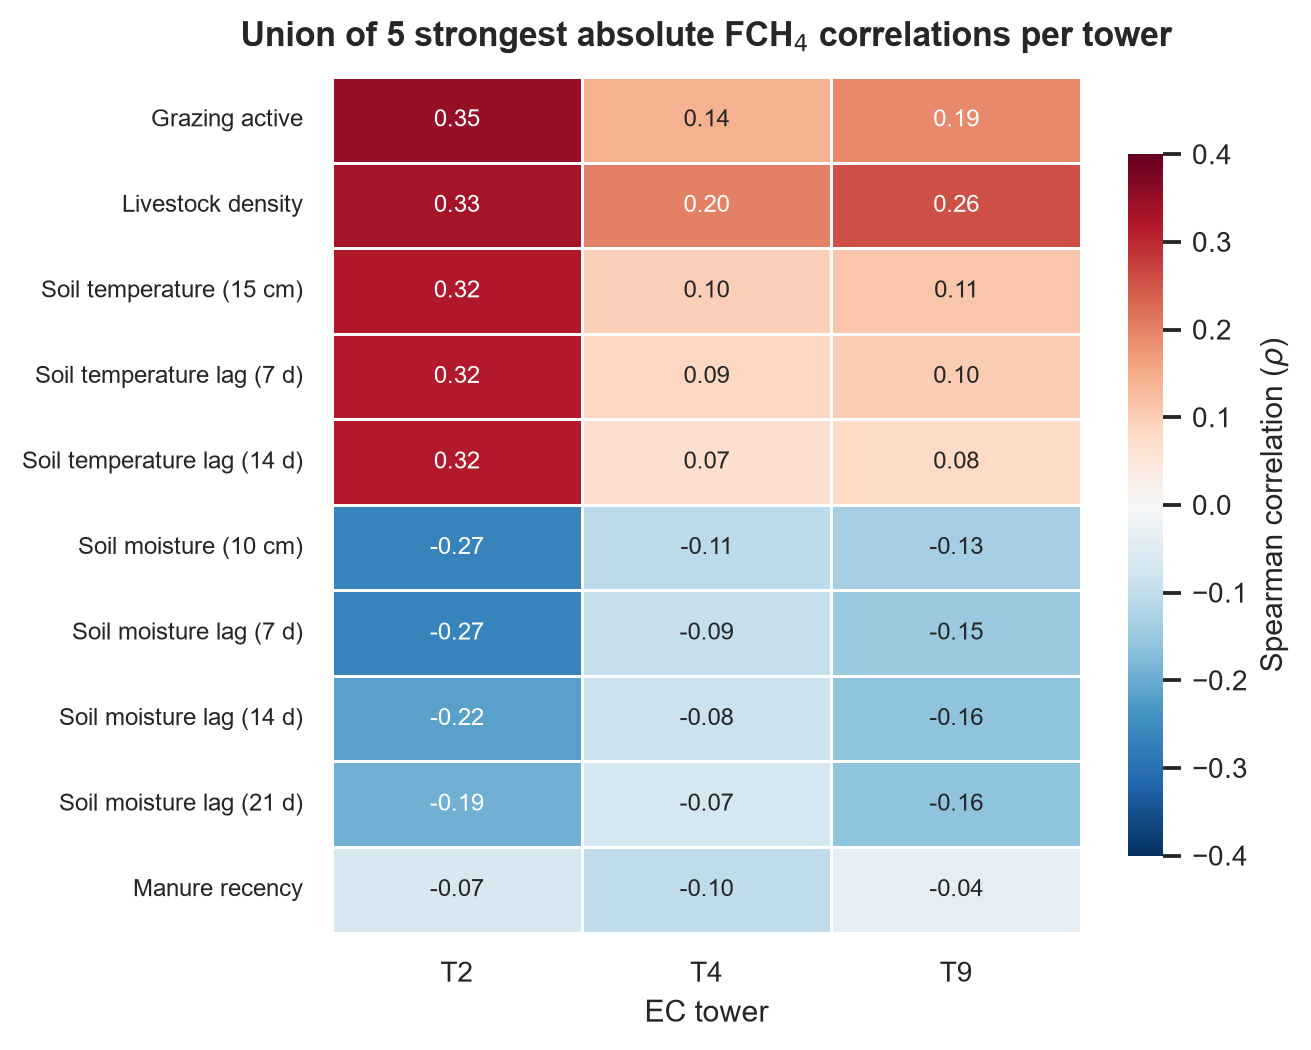
\includegraphics[width=0.82\textwidth]{Figures/ch3_fch4_target_correlations.png}
\caption{Strongest Spearman associations between observed QC-valid FCH\textsubscript{4} and the
gap-filling predictors. The displayed variables are the union of the five largest absolute
correlations selected independently within each EC tower; coefficients for all three towers are
then shown for every selected variable. Positive values indicate that larger predictor values tend
to accompany larger methane fluxes, whereas negative values indicate an inverse monotonic
association.}
\label{fig:ch3_target_correlations}
\end{figure}

Figure~\ref{fig:ch3_target_correlations} shows that livestock density has the strongest consistent
positive association across the three towers ($\rho=0.33$, $0.20$, and $0.26$ at T2, T4, and T9,
respectively), with grazing status showing the same direction. Soil moisture and its lagged values
are generally negatively associated with FCH\textsubscript{4}, whereas soil temperature is
positively associated, particularly at T2. However, all absolute correlations remain below 0.35
and their magnitudes differ substantially by tower. These coefficients therefore provide an
initial screening of the feature space rather than a feature-importance result: they do not capture
nonlinear interactions, and the closely related soil-lag variables share overlapping information.

Multivariate structure was examined using the same 11 environmental drivers employed by the
gap-filling pipeline. TICA \cite{perezhernandez2013} was fitted at a 24-hour lag after standardisation, 
treating each tower as a separate contiguous trajectory so that lagged pairs could not cross tower or deployment
boundaries. UMAP \cite{mcinnes2018umap} was fitted to a tower-balanced sample of 3,000 hours using 30 neighbours and a
minimum distance of 0.15. Neither analysis used FCH\textsubscript{4}, tower indicators, deterministic
calendar encodings or precomputed lag features as inputs; methane availability was introduced only
after fitting as a visual label. 

\begin{figure}[htbp]
\centering
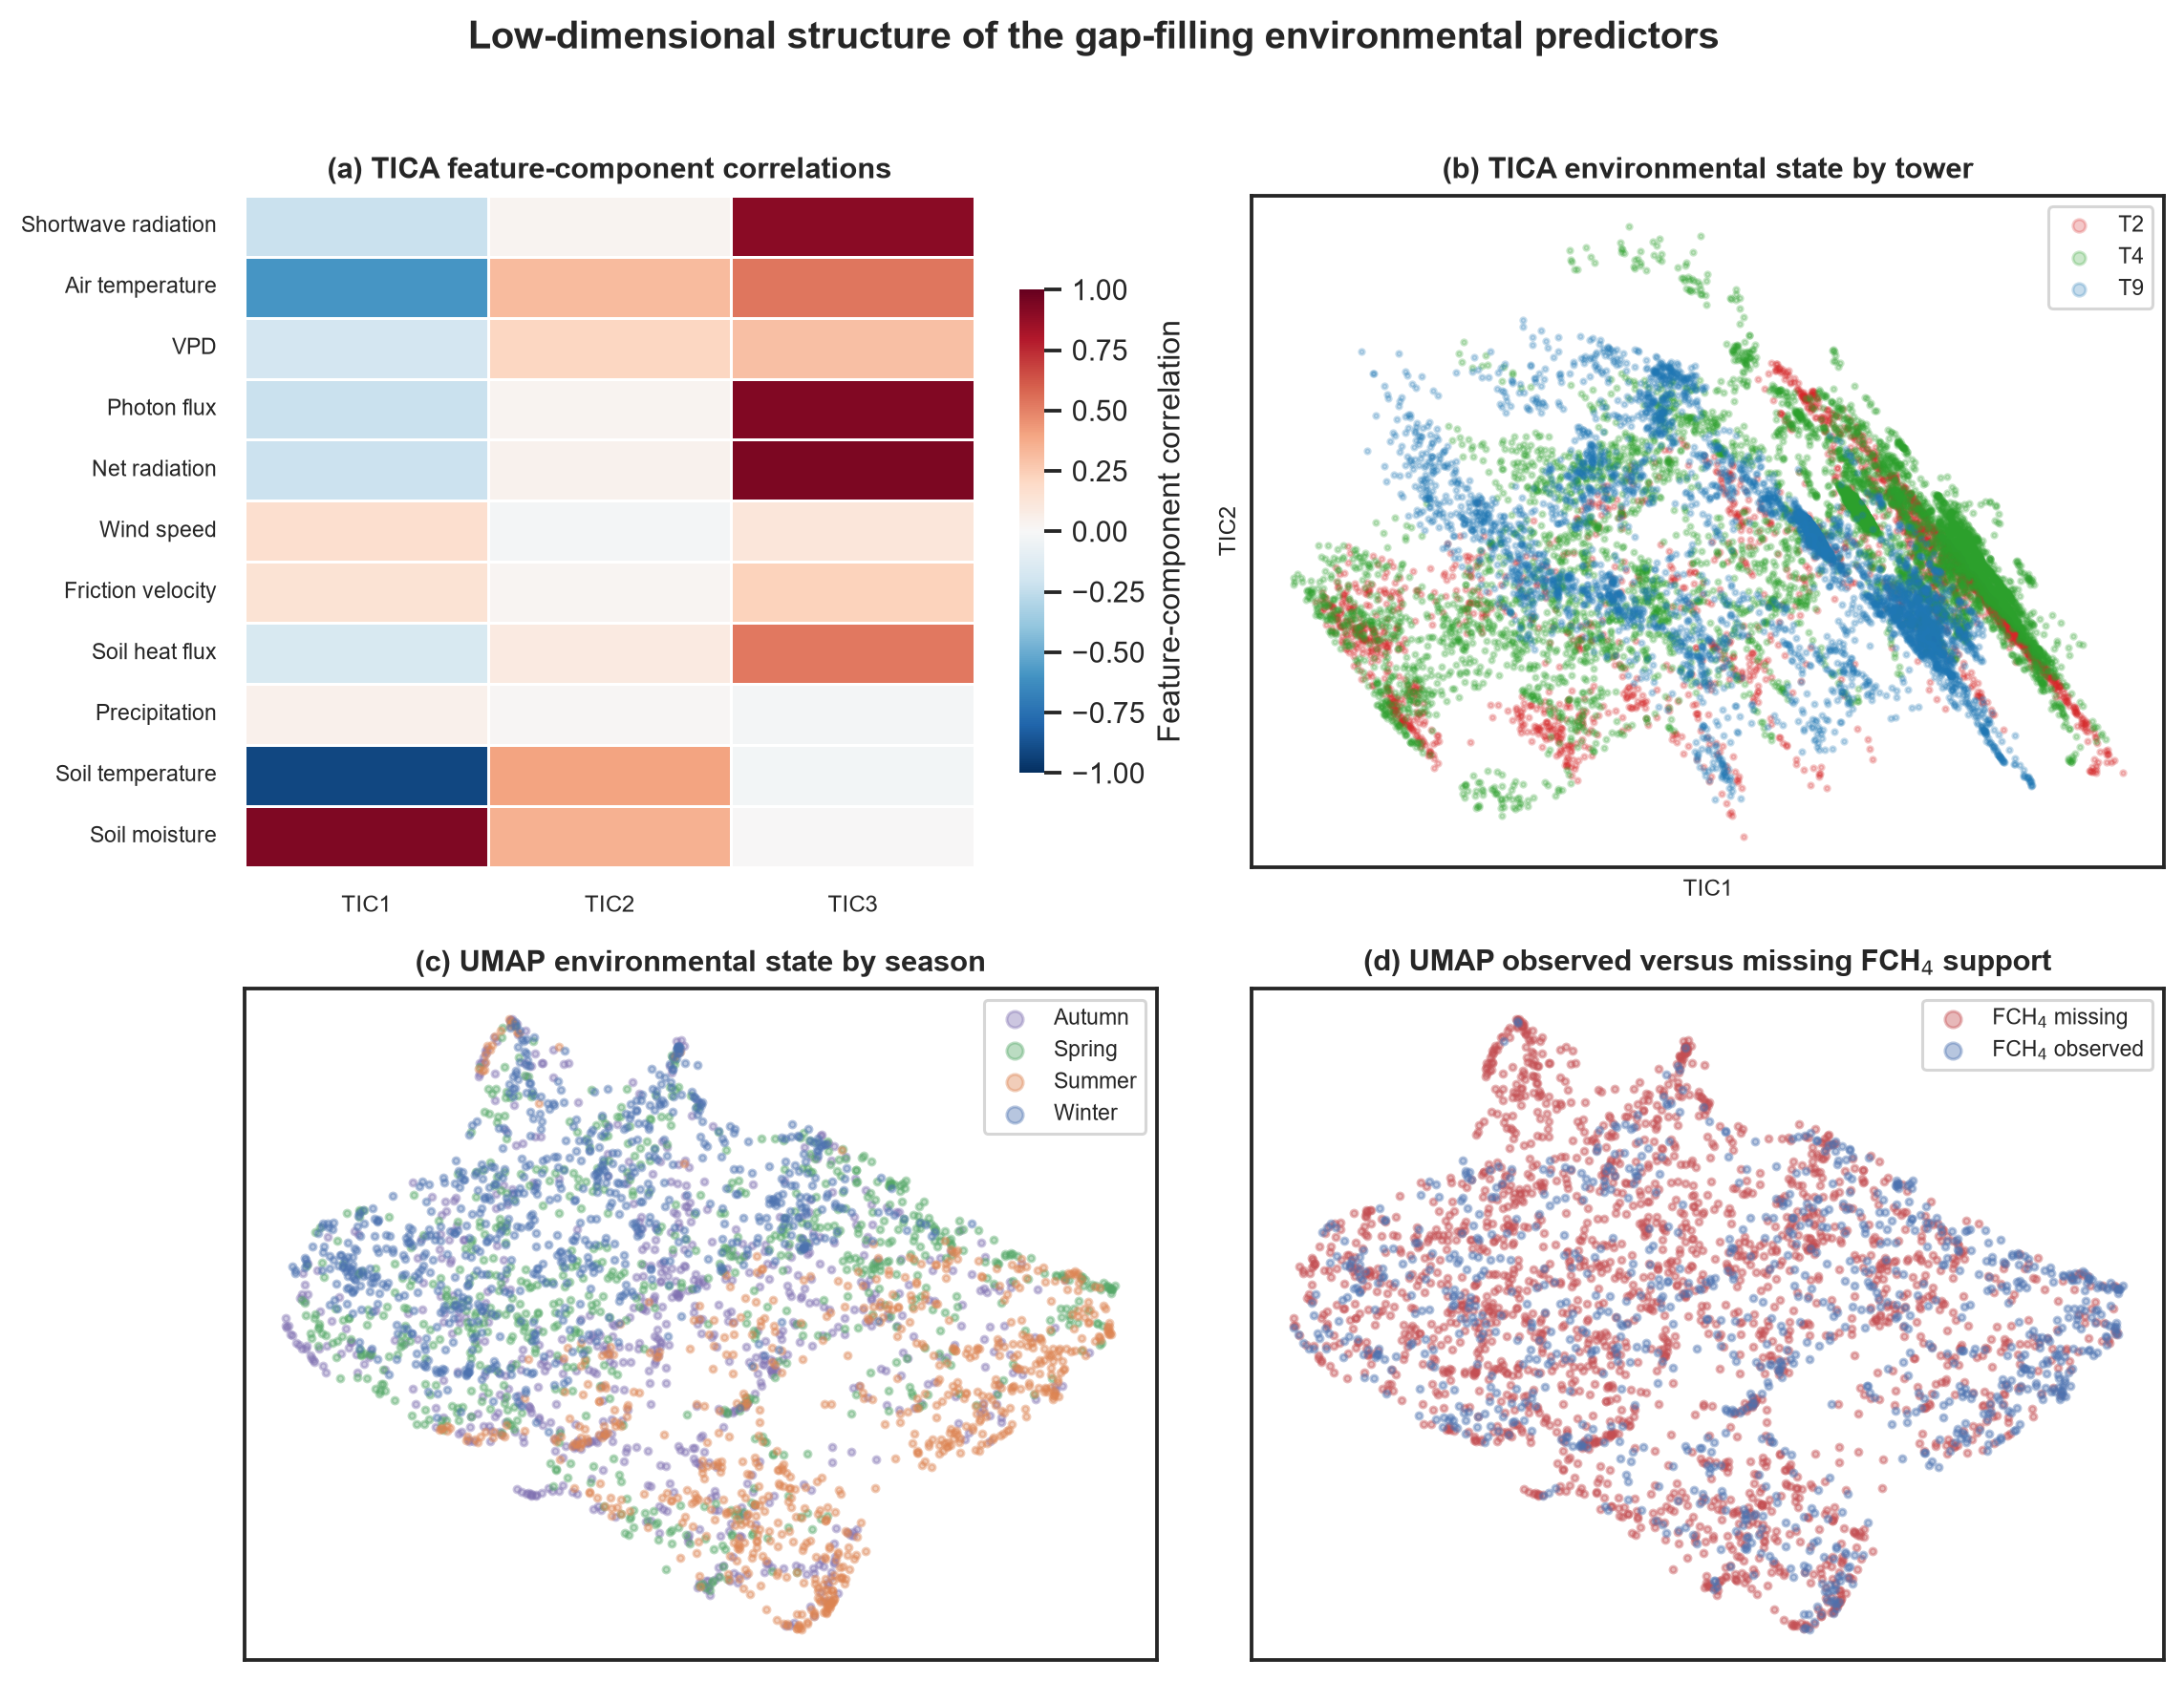
\includegraphics[width=\textwidth]{Figures/ch3_tica_umap_embeddings.png}
\caption{Low-dimensional structure of the environmental predictors used by the gap-filling
pipeline. Panel (a) shows feature--component correlations for three TICA components at a 24-hour
lag; panel (b) shows the first two TICA components by EC tower. Panels (c) and (d) show the same
saved UMAP embedding coloured by season and by observed versus missing FCH\textsubscript{4},
respectively. }
\label{fig:ch3_tica_umap}
\end{figure}

At a 24-hour lag, the first three TICA components had autocorrelations of 0.992, 0.970 and 0.869, 
implying timescales of 122, 33 and 7 days. The slowest component correlated 
strongly with soil moisture (0.93), soil temperature (0.91) and air temperature (0.59). UMAP showed 
moderate clustering by tower and season, but little separation between observed and missing FCH\textsubscript{4} 
hours. The two groups therefore occupy overlapping environmental space, though this does 
not establish that target missingness is random.

These diagnostics informed the final predictor design, but their
low-dimensional representations were not retained. The observed temporal
dependence supports the use of multi-scale lagged and rolling environmental
variables, while fold-safe experiments found no consistent improvement from
adding TICA components or UMAP-informed neighbour features. The final
gap-filling and forecasting models therefore use the original environmental
variables.

%%%%%%%%%%%%%%%%%%%%%%%%%%%%%%%%%%%%%%%%%%%%%%%%%%%%%%%%%%%%%%%%%%%%%%%%%%%%%%%%
%%%%%%%%%%%%%%%%%%%%%%%%%%%%%%%%%%%%%%%%%%%%%%%%%%%%%%%%%%%%%%%%%%%%%%%%%%%%%%%%%%%%%%%%%%%%%%%%%%%%%%%%
\chapter{Models and Methods}
\label{ChapModels}

This chapter defines the common modelling and evaluation methodology used
throughout the gap-filling, forecasting and scenario-projection experiments.
Although these tasks use the same underlying NWFP data, they represent
different prediction settings. Gap-filling reconstructs observations removed
from within an historical record, forecasting predicts beyond a defined
forecast origin, and scenario projection evaluates a fitted model under
prescribed future environmental and management conditions. The corresponding
validation procedures are therefore described separately before introducing
the complete model roster, uncertainty-quantification framework and
interpretability method.

% This chapter collects every machine learning model, statistical baseline, uncertainty-quantification
% (UQ) method, and interpretability technique used anywhere in this dissertation, regardless of which
% downstream task (gap-filling, forecasting, or scenario projection) applies it. Chapters~\ref{Chap4}
% through~\ref{Chap6} assume the descriptions below and report only configuration, results, and
% task-specific discussion.

%%%%%%%%%%%%%%%%%%%%%%%%%%%%%%%%%%%%%%%%%%%%%%%%%%%%%%%%%%%%%%%%%%%%%%%%%%%%%%%%%%%%%%%%%%%%%%%%%%%%%%%%
\section{Evaluation Methods and Metrics}
\label{sec:evaluation_protocols}

The benchmark models optimise different internal objectives, including squared
error, absolute error, likelihood-based objectives and quantile loss.
Consequently, they were compared using common held-out evaluation metrics
rather than their model-specific training losses. Table~\ref{tab:task_protocols}
summarises the principal distinction between the three modelling tasks.

\begin{table}[htbp]
\centering
\small
\caption{Summary of the evaluation settings used in the dissertation.}
\label{tab:task_protocols}
\begin{tabular*}{\textwidth}{@{\extracolsep{\fill}}
>{\raggedright\arraybackslash}p{0.16\textwidth}
>{\raggedright\arraybackslash}p{0.28\textwidth}
>{\raggedright\arraybackslash}p{0.34\textwidth}
>{\raggedright\arraybackslash}p{0.14\textwidth}@{}}
\toprule
Task & Evaluation unit & Information available to the model & Primary metric \\
\midrule
Gap-filling &
Synthetic calendar gaps placed within the observed record &
Remaining observations and supporting variables before and after each gap &
$R^2$ \\
\addlinespace[0.5em]

Forecasting &
365-day prediction from five historical forecast origins &
Historical training data and realised supporting variables over the evaluation period &
Seasonal-mean-scaled MASE \\
\addlinespace[0.5em]

Scenario projection &
Conditional prediction under prescribed climate and management trajectories &
Historical training data and externally supplied scenario covariates &
Relative change from the reference scenario \\
\bottomrule
\end{tabular*}
\end{table}

\subsection{Gap-Filling Cross-Validation}

Gap-filling was evaluated as an interpolation problem over each tower's usable
measurement period. The evaluation domains were 1 October 2017--30 June 2019
for T2, 1 October 2017--31 December 2023 for T4, and
1 February 2020--31 December 2023 for T9. Only QC-valid observed
FCH\textsubscript{4} values within these domains were eligible for masking.

Five synthetic-gap scenarios were used: very short gaps of one hour, short
gaps of four hours, medium gaps of 32 hours, long gaps of 288 hours, and a
mixed scenario in which gap length was sampled from these four durations.
Non-overlapping calendar gaps were positioned randomly until approximately
25\% of the available target observations had been masked. Two independently
seeded repetitions were evaluated for each tower and gap scenario.

For every repetition, the masked FCH\textsubscript{4} observations were removed
before fitting the model. Supporting environmental and management variables
remained available, and the model could use historical context from either
side of a gap. This reflects the intended use of gap-filling, in which later
observations may be available when an earlier missing interval is
reconstructed. It is therefore distinct from prospective forecasting and
should not be interpreted as evidence of future predictive skill.

Metrics were first calculated independently for each repetition. The median
over repetitions was then calculated within each gap-duration scenario,
followed by the median across the five scenarios. This prevents a particularly
large or easy synthetic gap from dominating the headline result. Where a
combined value is reported across T2, T4 and T9, the tower-level results are
averaged with equal weight so that the longer T4 record does not automatically dominate
the comparison.


\subsection{Forecasting Cross-Validation}

Forecasting was evaluated through fixed-origin backtesting. Five forecast
origins were defined on 16 December in 2018, 2019, 2020, 2021 and 2022.
At each origin, a model was fitted using only data available on or before that
date and generated a continuous 365-day daily prediction. Tower--origin
combinations without sufficient historical or observed evaluation data were
excluded rather than assigned artificial scores.

The resulting forecasts were evaluated against QC-valid observed
FCH\textsubscript{4}, not against the reconstructed target series. The
gap-filled historical series could be used to initialise autoregressive
features, but predictions were scored only where a real observation was
available. This prevents agreement with the gap-filling model from being
mistaken for agreement with measured methane flux.

For recursive models, each predicted FCH\textsubscript{4} value was appended
to the available history and used to construct the autoregressive inputs for
subsequent days. No later observed methane value was inserted during the
365-day rollout. Direct tabular foundation-model configurations instead
predicted from the available covariate representation without requiring the
same recursive target-update mechanism.

Historical backtests supplied the realised supporting environmental variables
over each future evaluation window. The resulting experiment is therefore a
conditional methane-flux forecast: it evaluates the mapping from environmental
and management conditions to FCH\textsubscript{4}, together with any recursive
target dependence, rather than simultaneously evaluating a separate weather
forecast. Future climate variables are supplied by the climate-scenario data
in the scenario-projection experiment.

Performance was additionally divided into lead-time intervals of 1--7,
8--30, 31--90, 91--180, 181--270 and 271--365 days. This permits degradation
with forecast horizon to be distinguished from overall performance. Aggregate
metrics are weighted by the number of observed target values contributing to
each tower--origin--horizon cell, ensuring that cells containing very few real
observations do not receive the same influence as well-observed cells.

\subsection{Scenario-Projection Evaluation}

Scenario projection has no observed future target and is therefore treated as
a conditional projection rather than a forecast-validation exercise. The
best-performing forecasting configuration is held fixed across all prescribed
climate and management trajectories, which are compared with a common
reference over the same projection period.

For scenario \(s\), the relative change in mean predicted
FCH\textsubscript{4} is calculated as

\begin{equation}
\Delta_s
=
100
\left(
\frac{
\overline{\hat{y}}_s-\overline{\hat{y}}_{\mathrm{ref}}
}{
\overline{\hat{y}}_{\mathrm{ref}}
}
\right),
\end{equation}

where \(\overline{\hat{y}}_s\) and
\(\overline{\hat{y}}_{\mathrm{ref}}\) denote the mean predictions under the
scenario and reference trajectories, respectively. These values quantify
modelled conditional differences and are not interpreted as validated
forecasts of future methane flux.

\subsection{Prediction Metrics}

Let \(y_i\) denote an observed flux and \(\hat{y}_i\) the corresponding model
prediction for \(n\) valid evaluation observations. Mean absolute error and
root mean squared error were calculated as

\begin{equation}
\mathrm{MAE}
=
\frac{1}{n}
\sum_{i=1}^{n}
\left|y_i-\hat{y}_i\right|,
\end{equation}

and

\begin{equation}
\mathrm{RMSE}
=
\sqrt{
\frac{1}{n}
\sum_{i=1}^{n}
\left(y_i-\hat{y}_i\right)^2
}.
\end{equation}

MAE represents the typical absolute error in the original flux units, whereas
RMSE gives greater weight to the comparatively rare large errors associated
with methane peaks.

Gap-filling primarily follows the OLS \(R^2\) convention used by the published
NWFP comparator \cite{zhu2023a}. In the implemented evaluation, this is the
squared Pearson correlation between observations and predictions:

\begin{equation}
R^2 (OLS)
=
\left[
\frac{
\sum_{i=1}^{n}
(y_i-\bar{y})
(\hat{y}_i-\bar{\hat{y}})
}{
\sqrt{
\sum_{i=1}^{n}(y_i-\bar{y})^2
\sum_{i=1}^{n}(\hat{y}_i-\bar{\hat{y}})^2
}
}
\right]^2.
\label{eq:r2_ols}
\end{equation}

Unlike the residual coefficient of determination
\(1-\sum(y_i-\hat{y}_i)^2/\sum(y_i-\bar{y})^2\),
Equation~\ref{eq:r2_ols} is bounded between zero and one. It measures the
strength of linear agreement but is comparatively insensitive to additive
bias and scale error. MAE and RMSE are therefore retained as supporting
metrics so that a model cannot be assessed from correlation alone.

Forecasting uses a seasonal-mean-scaled form of mean absolute scaled error.
For each forecast origin, the reference prediction for a target date is the
mean observed FCH\textsubscript{4} for the corresponding day of year within a
circular \(\pm 7\)-day window, calculated exclusively from observations before
the forecast origin. The reported metric is

\begin{equation}
\mathrm{MASE}_{\mathrm{seasonal}}
=
\frac{
\mathrm{MAE}(y,\hat{y})
}{
\mathrm{MAE}(y,\hat{y}^{\,\mathrm{seasonal}})
}.
\label{eq:mase_seasonal}
\end{equation}

This applies the scale-free comparison principle of MASE
\cite{hyndman2006accuracy} using the historical seasonal mean as the explicit
reference forecast. Values below one indicate that the model improves on the
seasonal mean, a value of one indicates equal error, and values above one
indicate inferior performance.

Weighted absolute percentage error was calculated as

\begin{equation}
\mathrm{WAPE}
=
\frac{
\sum_{i=1}^{n}|y_i-\hat{y}_i|
}{
\sum_{i=1}^{n}|y_i|
}.
\end{equation}

WAPE is more stable than observation-wise percentage errors for this
application because FCH\textsubscript{4} is signed and frequently lies near
zero. Pearson correlation was also reported to describe agreement in temporal
variation independently of absolute calibration. No single metric is treated
as sufficient: MASE provides the primary forecasting comparison, while MAE,
RMSE, WAPE and correlation identify differences in scale, peak sensitivity and
temporal tracking.

\section{Models Used}
\label{sec:model_roster}

The benchmark intentionally includes simple baselines, conventional statistical
models, tree ensembles, locally trained neural architectures and pretrained
tabular foundation models. This breadth permits the claim that one model
family outperforms another to be tested empirically under common evaluation
conditions. Table~\ref{tab:model_roster} summarises how each model operates and
where it is used. ``GF'' and ``FC'' denote gap-filling and forecasting 
respectively.

% {
% \small
% \setlength{\tabcolsep}{4pt}
% \renewcommand{\arraystretch}{1.15}
% \begin{longtable}{
% @{}
% >{\raggedright\arraybackslash}p{0.17\textwidth}
% >{\raggedright\arraybackslash}p{0.60\textwidth}
% >{\raggedright\arraybackslash}p{0.15\textwidth}
% @{}
% }
% \caption{Model families and their roles in the dissertation.}
% \label{tab:model_roster}\\
% \toprule
% Model & Operating principle & Application \\
% \midrule
% \endfirsthead

% \multicolumn{3}{l}{\tablename\ \thetable\ -- continued}\\
% \toprule
% Model & Operating principle & Application \\
% \midrule
% \endhead

% \midrule
% \multicolumn{3}{r}{Continued on next page}\\
% \endfoot

% \bottomrule
% \endlastfoot

% Training-set mean &
% Predicts the arithmetic mean of the available training target for every
% held-out observation. It contains no temporal, environmental or management
% information and therefore provides a zero-information reference against which
% all fitted gap-filling models should improve. &
% GF \\

% Marginal Distribution Sampling &
% Fills a target from observations recorded under similar meteorological
% conditions \cite{wutzler2018reddyproc}. The implemented hierarchy first
% searches for observations with comparable shortwave radiation, air temperature
% and VPD; then relaxes the search to shortwave radiation; and finally uses an
% expanding mean-diurnal-course fallback. Unlike a fitted regression model, MDS
% constructs each estimate by averaging conditionally similar historical
% observations. &
% GF \\

% MICE &
% Uses multivariate imputation by chained equations. Each incomplete variable is
% treated in turn as a regression target conditional on the remaining variables,
% and the procedure cycles through the columns iteratively. The implementation
% uses Bayesian ridge regression as the fixed conditional estimator. Masked
% FCH\textsubscript{4} values are recovered from the jointly imputed
% feature--target matrix. &
% GF \\

% HyperImpute &
% Retains the chained-equations structure of MICE but replaces its single fixed
% conditional estimator with an AutoML search. A separate regression or
% classification algorithm may therefore be selected for each imputed column.
% This allows nonlinear and variable-specific relationships to be represented,
% at substantially greater computational cost. &
% GF \\

% Random Forest &
% Fits many regression trees to bootstrap samples of the training data while
% considering a random subset of predictors at each split. Individual trees
% capture nonlinear thresholds and interactions, while averaging their
% predictions reduces variance. A meteorology-only configuration reproduces the
% published baseline, whereas the expanded configuration includes environmental,
% calendar, livestock and management features. Cross-tower versions use tower
% indicators to distinguish the three measurement contexts. &
% GF, FC \\

% XGBoost &
% Constructs regression trees sequentially. Each new tree is fitted to improve
% the residual errors of the existing ensemble, while shrinkage, tree-depth
% constraints and explicit regularisation limit overfitting. Its sequential
% error-correction mechanism can model nonlinear feature interactions but may
% remain sensitive to sparse methane peaks. &
% GF, FC \\

% LightGBM &
% Also uses gradient-boosted decision trees, but relies on histogram-based split
% search and leaf-wise tree growth. Histogram binning reduces computational cost,
% while leaf-wise growth expands the branch offering the greatest loss
% reduction. Depth and leaf-size restrictions are used to control the resulting
% model complexity. &
% GF, FC \\

% Artificial Neural Network &
% Passes the input features through successive fully connected nonlinear layers
% and learns their weights through gradient-based optimisation. The ANN appears
% in the published-baseline replication rather than the final improved
% gap-filling roster, permitting comparison with earlier methane-flux studies. &
% GF replication \\

% Support Vector Machine &
% Uses support-vector regression to estimate a function within an
% \(\epsilon\)-insensitive error tube. Kernel transformations permit nonlinear
% relationships to be represented through similarities between observations,
% while the regularisation parameter controls the balance between a flatter
% function and errors outside the tube. It is retained only for published
% baseline replication. &
% GF replication \\

% SAITS &
% A self-attention architecture designed specifically for multivariate
% time-series imputation \cite{du2023saits}. Two diagonally masked
% self-attention blocks learn relationships between variables and time points
% without directly copying the value being reconstructed. Their estimates are
% combined through a learned weighting mechanism and trained using observed-value
% reconstruction and artificial-masking objectives. &
% GF \\

% LSTM and Bi-LSTM &
% Long short-term memory networks maintain a recurrent cell state controlled by
% input, forget and output gates. These gates regulate which historical
% information is stored, removed and exposed to the prediction layer. The
% bidirectional gap-filling model processes a sequence in both temporal
% directions, which is appropriate when observations after a historical gap are
% available. The forecasting LSTM is causal at inference and updates its input
% history using earlier predictions during recursive rollout. &
% GF, FC \\

% Temporal Fusion Transformer &
% Combines recurrent local processing with variable-selection networks, gated
% residual components and attention over the encoded sequence. Variable-selection
% weights allow the model to emphasise different observed and known-future
% inputs, while attention represents longer temporal relationships. The
% forecasting implementation uses a fixed historical lookback and produces a
% multi-step sequence, of which the next prediction is introduced into the
% recursive chain. &
% FC \\

% DLinear &
% Decomposes each input sequence into a moving-average trend and a residual
% seasonal component, then applies separate linear projections to the two
% components \cite{zeng2023}. The final forecast is their sum. It provides a
% deliberately simple neural forecasting baseline for testing whether elaborate
% attention or recurrent architectures are necessary. &
% FC \\

% SARIMAX &
% Represents the target through autoregressive terms, differencing and
% moving-average error terms, together with exogenous environmental and
% management regressors. Candidate autoregressive and moving-average orders are
% fitted separately at each tower and forecast origin, with the final order
% selected using AIC. SARIMAX provides a classical statistical comparison with
% the machine-learning models. &
% FC \\

% TabPFN &
% A pretrained tabular foundation model that learns a prediction procedure from
% large numbers of synthetic tabular tasks
% \cite{hollmann2023tabpfn,hollmann2025tabpfn}. At inference, labelled historical
% rows form an in-context training set and unlabelled rows form prediction
% queries. Transformer attention relates the queries to the supplied context,
% producing point and quantile predictions without conventional task-specific
% gradient training. For forecasting, temporal structure is supplied through
% calendar, lagged, environmental and management features, following the
% tabularisation principle used by TabPFN-TS \cite{hoo2026tabpfnts}. &
% GF, FC \\

% TabICLv2 &
% Extends tabular in-context learning to larger tabular contexts through revised
% synthetic pretraining and scalable attention
% \cite{qu2025tabicl,qu2026tabiclv2}. As with TabPFN, labelled context rows and
% query rows are processed jointly at inference. In gap-filling it is fitted
% separately by tower because its fixed context budget can be diluted by pooling.
% The scenario model also uses a per-tower direct-regression configuration with
% a restricted climate-compatible feature set. &
% GF, FC, SP \\

% Prediction ensemble &
% Combines predictions from independently fitted models. The forecasting
% benchmark evaluates an unweighted mean of Random Forest, XGBoost, LightGBM and
% SARIMAX, while the final TabPFN combination averages complementary TabPFN
% configurations. Averaging can reduce model-specific variance, although it can
% also dilute a stronger constituent with weaker members. &
% FC \\
% \end{longtable}
% }

  {
  \small
  \setlength{\tabcolsep}{4pt}
  \renewcommand{\arraystretch}{1.13}
  \begin{longtable}{
  @{}
  >{\raggedright\arraybackslash}p{0.17\textwidth}
  >{\raggedright\arraybackslash}p{0.60\textwidth}
  >{\raggedright\arraybackslash}p{0.15\textwidth}
  @{}
  }
  \caption{Model families and their roles in the dissertation.}
  \label{tab:model_roster}\\
  \toprule
  Model & Operating principle & Application \\
  \midrule
  \endfirsthead

  \multicolumn{3}{l}{\tablename\ \thetable\ -- continued}\\
  \toprule
  Model & Operating principle & Application \\
  \midrule
  \endhead

  \midrule
  \multicolumn{3}{r}{Continued on next page}\\
  \endfoot

  \bottomrule
  \endlastfoot

  Training-set mean &
  Predicts the mean observed training target for every held-out row, providing a
  zero-information reference. &
  GF \\

  MDS &
  Reconstructs flux from historical observations under similar meteorological
  conditions, followed by an expanding mean-diurnal-course fallback
  \cite{reichstein2005mds,wutzler2018reddyproc,zhu2023a}. &
  GF \\

  MICE &
  Iteratively predicts each incomplete variable from the remaining variables.
  The implementation uses Bayesian ridge regression as the conditional estimator
  \cite{vanbuuren2011mice}. &
  GF \\

  HyperImpute &
  Extends chained-equation imputation by using an AutoML search to select a
  conditional estimator separately for each variable
  \cite{jarrett2022hyperimpute}. &
  GF \\

  Random Forest &
  Averages regression trees fitted to bootstrap samples with random feature
  selection at each split, capturing nonlinearities while reducing individual-tree
  variance \cite{breiman2001randomforests,irvin2021,kim2020,zhu2023a}. &
  GF, FC \\

  XGBoost &
  Builds regularised regression trees sequentially, with each tree correcting
  residual errors left by the existing ensemble
  \cite{chen2016xgboost,irvin2021}. &
  GF, FC \\

  LightGBM &
  Uses histogram-based gradient boosting and leaf-wise tree growth to model
  nonlinear relationships efficiently \cite{ke2017lightgbm}. &
  GF, FC \\

  ANN &
  Learns nonlinear feature combinations through successive fully connected
  layers trained by gradient-based optimisation
  \cite{rumelhart1986backprop,kim2020}. &
  GF replication \\

  SVM &
  Uses support-vector regression to fit a regularised function within an
  $\epsilon$-insensitive error margin, with kernels permitting nonlinear
  relationships \cite{drucker1997svr,kim2020}. &
  GF replication \\

  SAITS &
  Uses diagonally masked self-attention blocks and learned combination weights
  to reconstruct multivariate time-series gaps \cite{du2023saits}. &
  GF \\

  LSTM and Bi-LSTM &
  Use gated recurrent memory to retain or discard temporal information.
  Bi-LSTM uses context on both sides of a historical gap, whereas forecasting
  LSTM operates causally during rollout
  \cite{hochreiter1997lstm,schuster1997bidirectional}. &
  GF, FC \\

  TFT &
  Combines recurrent processing, variable-selection networks, gating and
  temporal attention to represent local and longer-range forecasting
  relationships \cite{lim2021tft}. &
  FC \\

  DLinear &
  Decomposes a sequence into trend and residual components and forecasts each
  with a linear projection \cite{zeng2023}. &
  FC \\

  SARIMAX &
  Combines autoregressive, differencing and moving-average terms with exogenous
  environmental and management regressors. Candidate orders are selected using
  AIC \cite{box2015timeseries}. &
  FC \\

  TabPFN &
  Uses a transformer pretrained on synthetic tabular tasks to infer predictions
  from labelled context rows and unlabelled query rows
  \cite{hollmann2023tabpfn,hollmann2025tabpfn}. Temporal prediction is represented
  through engineered time-series features \cite{hoo2026tabpfnts}. &
  GF, FC \\

  TabICLv2 &
  Uses scalable tabular in-context learning with synthetic pretraining
  \cite{qu2025tabicl,qu2026tabiclv2}. &
  GF, FC \\

  Prediction ensemble &
  Averages predictions from complementary fitted models to reduce
  model-specific variance. Both tree--statistical and TabPFN combinations are
  evaluated \cite{bates1969combination}. &
  FC \\

  \end{longtable}
  }

For locally fitted tabular models, missing predictor values were replaced using
statistics estimated from the corresponding training data. Pooled models used
tower indicators to share information while retaining tower-specific effects.
Exact feature configurations, context lengths and hyperparameters are reported
with the corresponding experiments; Table~\ref{tab:model_roster} defines only 
the common operating principles used throughout the results chapters.

% For locally fitted tabular models, missing predictor values were replaced using
% statistics estimated from the corresponding training data. Where models were
% pooled across towers, tower-indicator variables allowed a common fitted
% function to retain tower identity. This differs from treating the three towers
% as interchangeable observations: pooling shares statistical information while
% still permitting tower-specific offsets and interactions.

% Exact feature configurations, context lengths and hyperparameters are reported
% with the corresponding gap-filling, forecasting and scenario-projection
% experiments. The purpose of Table~\ref{tab:model_roster} is to define the
% operating principles of the models once, avoiding repeated generic
% descriptions in each results chapter.



%%%%%%%%%%%%%%%%%%%%%%%%%%%%%%%%%%%%%%%%%%%%%%%%%%%%%%%%%%%%%%%%%%%%%%%%%%%%%%%%%%%%%%%%%%%%%%%%%%%%%%%%
\section{Uncertainty Quantification}
\label{sec:uncertainty_methods}

Point predictions alone do not distinguish confident predictions from periods
in which multiple methane outcomes are plausible. Uncertainty was therefore
represented through quantile-based machine learning and conformal calibration.
For a conditional target distribution \(Y\mid X=x\), the quantile model
estimates

\begin{equation}
Q_{\tau}(x)
=
\inf\left\{
y:
P(Y\leq y\mid X=x)\geq\tau
\right\},
\end{equation}

where \(\tau\in(0,1)\) denotes the desired quantile. The experiments use
\(\tau=0.05\), \(0.50\) and \(0.95\), producing a median point prediction and a
nominal 90\% interval.

Quantile models are trained or evaluated using pinball loss
\cite{koenker1978quantiles}:

\begin{equation}
L_{\tau}(y,\hat{q}_{\tau})
=
\begin{cases}
\tau(y-\hat{q}_{\tau}),
& y\geq\hat{q}_{\tau},\\
(1-\tau)(\hat{q}_{\tau}-y),
& y<\hat{q}_{\tau}.
\end{cases}
\label{eq:pinball}
\end{equation}

The asymmetric weighting means that underprediction is penalised more heavily
for a high quantile and overprediction more heavily for a low quantile.
Minimising Equation~\ref{eq:pinball} therefore estimates the corresponding
conditional quantile rather than the conditional mean.

% Several mechanisms were used to obtain initial intervals. Quantile Regression
% Forest derives quantiles from the distribution of training outcomes represented
% within the fitted forest leaves. XGBoost and LightGBM fit separate
% quantile-objective models for the 0.05, 0.50 and 0.95 levels. SARIMAX obtains
% intervals from its fitted state-space forecast distribution, while the TFT
% uses a quantile-output head. TabPFN and TabICLv2 provide native predictive
% quantiles from their pretrained regression distributions. Where an ensemble
% was evaluated, corresponding lower, median and upper predictions from its
% constituent models were combined using the same weights as the point ensemble.

Several mechanisms were used to obtain initial prediction intervals. Quantile
Regression Forest estimates conditional quantiles from the distribution of
training outcomes represented within the fitted forest leaves
\cite{meinshausen2006qrf}. XGBoost and LightGBM fit separate
quantile-objective models for the 0.05, 0.50 and 0.95 levels, while SARIMAX
obtains intervals from its fitted state-space forecast distribution. The TFT
uses a quantile-output head, and TabPFN and TabICLv2 provide predictive
quantiles from their pretrained regression distributions. For an ensemble,
corresponding lower, median and upper predictions were combined using the same
weights as the point predictions.

Raw model quantiles are not guaranteed to achieve their nominal coverage on
NWFP data. Split-conformal calibration was therefore used to adjust the
intervals using held-out residual information
\cite{lei2018distributionfree}.
For symmetric split-conformal intervals, the calibration score for observation
\(i\) is

\begin{equation}
s_i
=
\left|
y_i-\hat{q}_{0.50}(x_i)
\right|.
\end{equation}

For a desired miscoverage rate \(\alpha=0.10\), the conformal margin is the
finite-sample corrected \(1-\alpha\) quantile of the calibration scores. The
calibrated interval is then

\begin{equation}
C_{0.90}(x)
=
\left[
\hat{q}_{0.50}(x)-\hat{s},
\hat{q}_{0.50}(x)+\hat{s}
\right].
\end{equation}

Forecasting calibration used a leave-one-anchor-out procedure. When one
forecast origin was evaluated, residuals from the remaining four origins were
pooled within the corresponding lead-time interval. The resulting conformal
margin was then applied to the held-out origin. This preserves separation
between calibration and evaluation while allowing interval width to vary
between short and long forecast horizons.

Conformalized Quantile Regression was additionally used where the native
quantile spread contained information that a symmetric interval around the
median would discard \cite{romano2019cqr}. Its nonconformity score is

\begin{equation}
s_i^{\mathrm{CQR}}
=
\max\left\{
\hat{q}_{0.05}(x_i)-y_i,\;
y_i-\hat{q}_{0.95}(x_i)
\right\},
\end{equation}

giving the calibrated interval

\begin{equation}
C^{\mathrm{CQR}}_{0.90}(x)
=
\left[
\hat{q}_{0.05}(x)-\hat{s}_{\mathrm{CQR}},
\hat{q}_{0.95}(x)+\hat{s}_{\mathrm{CQR}}
\right].
\end{equation}

For gap-filling, QRF and TabICLv2 intervals were evaluated on the synthetic
held-out gaps. Calibration data were separated from the interval-evaluation
data within each tower and gap-duration setting. For forecasting, calibration
was separated by forecast origin and lead-time interval. Scenario intervals
reuse margins learned from historical backtests; they quantify historically
calibrated predictive dispersion but cannot guarantee coverage under an
unobserved future distribution shift.

Let \(\hat{l}_i\) and \(\hat{u}_i\) denote the final lower and upper
bounds of the interval evaluated for observation \(i\). These may correspond
to either the raw model quantiles or their conformally calibrated
counterparts.

Three complementary interval metrics were reported. Prediction Interval
Coverage Probability is

\begin{equation}
\mathrm{PICP}
=
\frac{1}{n}
\sum_{i=1}^{n}
\mathbb{I}
\left(
\hat{l}_i
\leq y_i
\leq
\hat{u}_i
\right).
\end{equation}

This measures the proportion of observations inside the interval. For a nominal
90\% interval, values substantially below 0.90 indicate undercoverage and
overconfidence, whereas values well above 0.90 indicate conservative
intervals.

Mean Prediction Interval Width is

\begin{equation}
\mathrm{MPIW}
=
\frac{1}{n}
\sum_{i=1}^{n}
\left(
\hat{u}_i-\hat{l}_i
\right).
\end{equation}

MPIW measures sharpness. Narrower intervals are preferable only when their
coverage remains comparable; an arbitrarily narrow interval with poor PICP is
not useful. Mean pinball loss across the three quantiles measures the accuracy
of the quantile predictions. PICP, MPIW and pinball loss are
therefore interpreted jointly as coverage, sharpness and quantile accuracy,
respectively.

% ============================================================================
\section{Interpretability}
\label{sec:interpretability_methods}

Permutation-based prediction sensitivity was used as the common model-agnostic
interpretability method. For each forecast origin and tower, the fitted model
first produced an unmodified prediction vector
\(\hat{\mathbf{y}}\). Predictor \(j\) was then shuffled across the evaluation
rows and the already fitted model was applied again without retraining.

Sensitivity was calculated as

\begin{equation}
I_j
=
\left|
\frac{1}{n}
\sum_{i=1}^{n}
\hat{y}^{\,\pi(j)}_i
-
\frac{1}{n}
\sum_{i=1}^{n}
\hat{y}_i
\right|,
\label{eq:permutation_importance}
\end{equation}

where \(\hat{y}^{\,\pi(j)}_i\) is the prediction obtained after permuting
feature \(j\). The score therefore measures the change in mean predicted
FCH\textsubscript{4} caused by disrupting the information carried by that
feature. Unlike conventional error-based permutation importance
\cite{breiman2001randomforests}, it does not require an observed future target
and can consequently be applied to conditional scenario projections.

Permutations were performed within each tower so that values were not mixed
between T2, T4 and T9. Tower indicators were not permuted. Scores were
calculated across the five forecast origins using deterministic seeds and were
then summarised overall and by tower.

These scores measure model reliance rather than physical causality. Correlated
predictors may share importance, while permutation may create combinations of
variables that are uncommon in the observed data. Interpretation therefore
focuses on stable feature groups and cross-tower patterns rather than small
differences between individual rankings.

%%%%%%%%%%%%%%%%%%%%%%%%%%%%%%%%%%%%%%%%%%%%%%%%%%%%%%%%%%%%%%%%%%%%%%%%%%%%%%%%
\chapter{Gap-Filling} \label{Chap4}

\section{Overview}

Chapter~\ref{Chap3} showed that raw hourly FCH\textsubscript{4} was unavailable
for 86.8\%, 50.3\% and 71.5\% of the common analysis window at T2, T4 and T9,
respectively. After applying the target quality and plausibility criteria,
effective unavailability increased to 92.0\%, 68.3\% and 81.7\%
(Table~\ref{tab:ch3_fch4_missingness}). Chapter~\ref{Chap3} reconstructed the
supporting environmental variables to provide a complete predictor frame but
deliberately left FCH\textsubscript{4} unfilled. Reconstructing this remaining
target supports continuous retrospective analysis and downstream model
configurations that require an uninterrupted methane history.

The experiments use the tower-specific hourly modelling frames constructed in
Chapter~\ref{Chap3}. The response variable is QC-valid observed
FCH\textsubscript{4}, while the expanded predictor frame combines current
environmental conditions, carbon-cycle variables, calendar encodings,
livestock information, environmental history and management events.
Table~\ref{tab:gf_features} summarises these inputs.

\begin{table}[htbp]
\centering
\small
\renewcommand{\arraystretch}{1.15}
\caption{Expanded predictor frame used in the gap-filling benchmark. Counts
exclude the FCH\textsubscript{4} target and tower-indicator variables.}
\label{tab:gf_features}
\begin{tabular*}{\textwidth}{@{\extracolsep{\fill}}
>{\raggedright\arraybackslash}p{0.22\textwidth}
>{\raggedright\arraybackslash}p{0.63\textwidth}
>{\centering\arraybackslash}p{0.07\textwidth}@{}}
\toprule
Feature group & Variables & Count \\
\midrule
Current environmental conditions &
SWIN, TA, VPD, PPFD, RN, WS, USTAR, SHF, precipitation,
soil temperature and soil moisture &
11 \\
\addlinespace[0.35em]

Carbon cycle &
Gap-filled FCO\textsubscript{2}, GPP and ecosystem respiration &
3 \\
\addlinespace[0.35em]

Calendar &
Cyclic hour-of-day and day-of-year sine and cosine encodings &
4 \\
\addlinespace[0.35em]

Livestock &
Livestock-unit density and grazing-presence indicator &
2 \\
\addlinespace[0.35em]

Environmental history &
Soil-moisture and soil-temperature lags at 168, 336, 504 and
672 hours &
8 \\
\addlinespace[0.35em]

Management &
Recency of cutting and manure application &
2 \\
\midrule
\textbf{Total} & & \textbf{30} \\
\bottomrule
\end{tabular*}
\end{table}

The expanded 30-predictor frame was used for the principal tabular benchmark.
Models sharing data across towers additionally received three tower-indicator
variables, whereas TabICLv2 did not require them.
MDS used only shortwave radiation, air temperature and VPD, while the
meteorology-only Random Forest used the 11 current environmental variables.
SAITS and Bi-LSTM omitted the eight explicit soil-lag variables because
temporal context was supplied directly through their input sequences.
Published-baseline replications retained their corresponding study-specific
feature subsets.

All models were evaluated using the synthetic-gap protocol defined in
Chapter~\ref{ChapModels}. Consequently, the reported scores measure recovery
of deliberately masked observations for which ground truth exists; they do not
establish that predictions made during naturally unobserved intervals are
equivalent to measurements. The following sections compare the complete model
roster against literature-aligned baselines and evaluate prediction-interval
calibration.

\FloatBarrier

\section{Results}

Unless otherwise stated, results are the median tower-specific \(R^2\) values,
calculated using the OLS convention defined in Chapter~\ref{ChapModels}, under
the common synthetic-gap protocol. Combined results are equal-weight
averages over T2, T4 and T9, preventing the longer T4 record from
dominating the comparison. Because this form of \(R^2\) measures linear
agreement rather than absolute calibration, the accompanying uncertainty
analysis is used to qualify the headline ranking.

\subsection{Full Model Comparison}

MDS and the meteorology-only Random Forest provide literature-aligned reference
points within the common benchmark, with Zhu et al. serving as the closest
same-site comparator \cite{zhu2023a}. Adaptations of the broader Irvin and Kim
benchmarks are retained in Appendix Table~\ref{tab:gf_published_replication} for
context rather than treated as controlled cross-study comparisons.

\begin{table}[htbp]
\centering
\footnotesize
\begin{tabular*}{\textwidth}{@{\extracolsep{\fill}}lrrrrr@{}}
\toprule
Model or experiment & T2 $R^2$ & T4 $R^2$ & T9 $R^2$ & Combined & \shortstack{Improvement\\over MDS} \\
\midrule
Training-set mean & -- & -- & -- & -- & -- \\
MDS & 0.072 & 0.038 & 0.054 & 0.055 & 0.000 \\
RF (meteorology features only) & 0.054 & 0.042 & 0.065 & 0.054 & $-0.001$ \\
MICE & 0.104 & 0.128 & 0.110 & 0.114 & $+0.059$ \\
HyperImpute & 0.567 & 0.352 & 0.362 & 0.427 & $+0.372$ \\
RF (additional features) & 0.601 & 0.409 & 0.430 & 0.480 & $+0.425$ \\
LightGBM & 0.583 & 0.418 & 0.425 & 0.475 & $+0.420$ \\
XGBoost & 0.619 & 0.380 & 0.375 & 0.458 & $+0.403$ \\
SAITS & 0.562 & 0.289 & 0.304 & 0.385 & $+0.330$ \\
Bidirectional LSTM & 0.280 & 0.204 & 0.189 & 0.224 & $+0.169$ \\
\textbf{TabICLv2} & \textbf{0.686} & \textbf{0.429} & \textbf{0.430} & \textbf{0.515} & $\mathbf{+0.460}$ \\
\bottomrule
\end{tabular*}
\caption{Full gap-filling model comparison under the common synthetic-gap
protocol. Combined values are equal-weight averages of the three
tower-specific \(R^2\) scores; improvement over MDS is the difference between
each model's combined score and the combined MDS score. The training-set mean
is constant, so its squared-correlation \(R^2\) is undefined.}
\label{tab:gf_model_comparison}
\end{table}

Table~\ref{tab:gf_model_comparison} shows that TabICLv2 produced the strongest
overall linear agreement, leading at T2 and T4, matching the expanded Random
Forest at T9, and attaining a combined \(R^2\) of 0.515. The
expanded Random Forest and LightGBM remained close at 0.480 and 0.475,
respectively, whereas MICE and the two deep sequence models were weaker. The
results therefore do not support a general claim that deep learning is
superior to traditional machine learning: performance depended on the model
architecture and its use of the available context. TabICLv2 is therefore
retained as the gap-filling champion.
Aggregate MAE and RMSE values for the same model comparison are reported in
Appendix Table~\ref{tab:gf_error_metrics_aggregate}.

Relative to MDS, the combined \(R^2\) increased by 0.425 for the expanded
Random Forest and 0.460 for TabICLv2; their tower-specific gains ranged from
0.371 to 0.614. These are reported as additive changes rather than percentage
gains because ratios against an \(R^2\) value close to zero would exaggerate
the apparent improvement.

\begin{figure}[htbp]
\centering
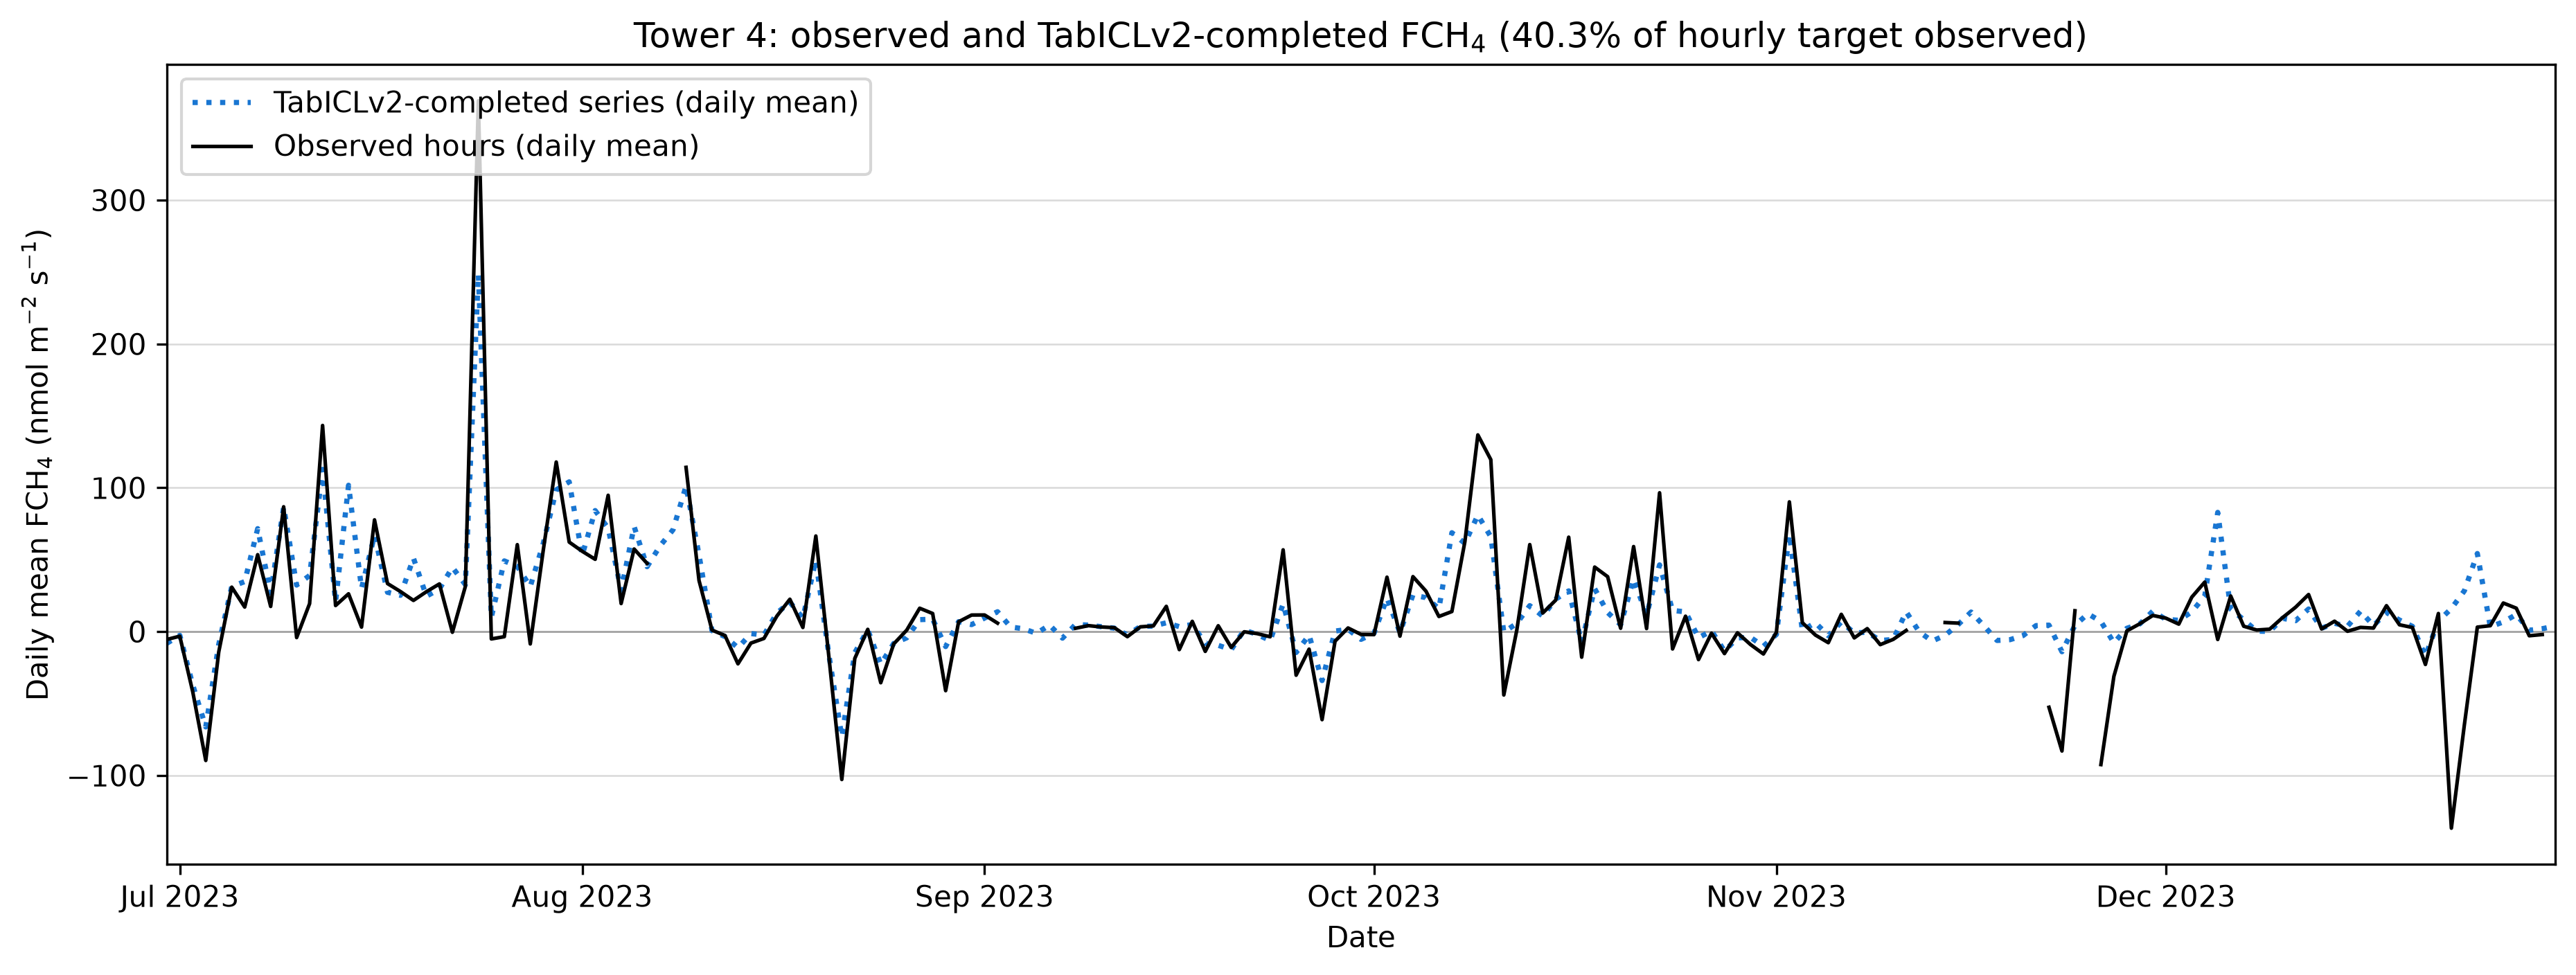
\includegraphics[width=\textwidth]{Figures/ch4_tabiclv2_daily_T4_2023H2.png}
\caption{Daily means of QC-valid observed hours (solid black) and the
TabICLv2-completed series (dotted blue) at T4 from July to December 2023, when
40.3\% of the hourly FCH\textsubscript{4} target was observed. The completed
series preserves observations and replaces missing hours with TabICLv2
estimates; the comparison is therefore a reconstruction diagnostic rather
than held-out validation. Corresponding T2 and T9 reconstructions are provided
in Appendix Figure~\ref{fig:app_gf_tabicl_daily_t2_t9}.}
\label{fig:gf_t4_reconstruction}
\end{figure}

Figure~\ref{fig:gf_t4_reconstruction} illustrates the operational effect of
applying TabICLv2 to a sparse measurement period. The completed series
provides a continuous daily trajectory and follows the broad observed
variation, although several peaks are attenuated. Its overlap with the
observed line is expected because measured hours are preserved rather than
replaced. The figure therefore demonstrates the operational reconstruction
while retaining the distinction between estimates and direct measurements.

\FloatBarrier

\subsection{Uncertainty Quantification} \label{gf:uq}
Raw 90\% prediction intervals were obtained from Quantile Regression Forests
for RFm and native quantile predictions for TabICLv2. Split-conformal
calibration was then evaluated separately within each tower and gap-duration
setting, following Chapter~\ref{ChapModels}.

\begin{table}[htbp]
\centering
\footnotesize
\begin{tabular*}{\textwidth}{@{\extracolsep{\fill}}llrrrrr@{}}
\toprule
Model & Tower & $n$ & \shortstack{Raw\\PICP} & \shortstack{Calibrated\\PICP} & \shortstack{Raw\\MPIW} & \shortstack{Calibrated\\MPIW} \\
\midrule
QRF (additional features) & T2 & 4,961 & 0.938 & 0.893 & 163.8 & 147.6 \\
 & T4 & 19,485 & 0.917 & 0.901 & 196.1 & 186.8 \\
 & T9 & 11,279 & 0.902 & 0.903 & 214.2 & 216.2 \\
 & \textbf{Average} & \textbf{35,725} & \textbf{0.919} & \textbf{0.899} & \textbf{191.4} & \textbf{183.5} \\
\addlinespace[0.3em]
TabICLv2 (quantile) & T2 & 4,961 & 0.918 & 0.904 & 134.5 & 130.1 \\
 & T4 & 19,485 & 0.899 & 0.899 & 181.6 & 181.2 \\
 & T9 & 11,279 & 0.888 & 0.893 & 214.5 & 217.2 \\
 & \textbf{Average} & \textbf{35,725} & \textbf{0.902} & \textbf{0.899} & \textbf{176.8} & \textbf{176.2} \\
\bottomrule
\end{tabular*}
\caption{Raw and split-conformal 90\% prediction-interval performance on the
held-out calibration-test subset of the synthetic-gap experiment. PICP has a
nominal target of 0.90; MPIW is reported in
\(\mathrm{nmol\,m^{-2}\,s^{-1}}\). Tower rows are equal-weight means across
the four gap-duration settings; averages weight all tower--gap cells
equally, while \(n\) reports their total test observations.}
\label{tab:gf_uq_calibration}
\end{table}

\FloatBarrier

Both raw interval methods were close to the 0.90 nominal target
(Table~\ref{tab:gf_uq_calibration}). Calibration reduced average QRF
coverage from 0.919 to 0.899 while narrowing MPIW from 191.4 to 183.5.
TabICLv2 moved from 0.902 to 0.899 coverage while MPIW changed only from 176.8
to 176.2. Across the
individual tower--gap cells, calibrated coverage ranged from 0.876 to 0.912
for QRF and from 0.888 to 0.910 for TabICLv2. Figure~\ref{fig:gf_tabicl_hourly_examples}
deliberately shows the raw native interval from the production chain; the
calibrated results in Table~\ref{tab:gf_uq_calibration} come from the separate
held-out synthetic-gap evaluation and were not applied to that chain.

\begin{figure}[htbp]
\centering
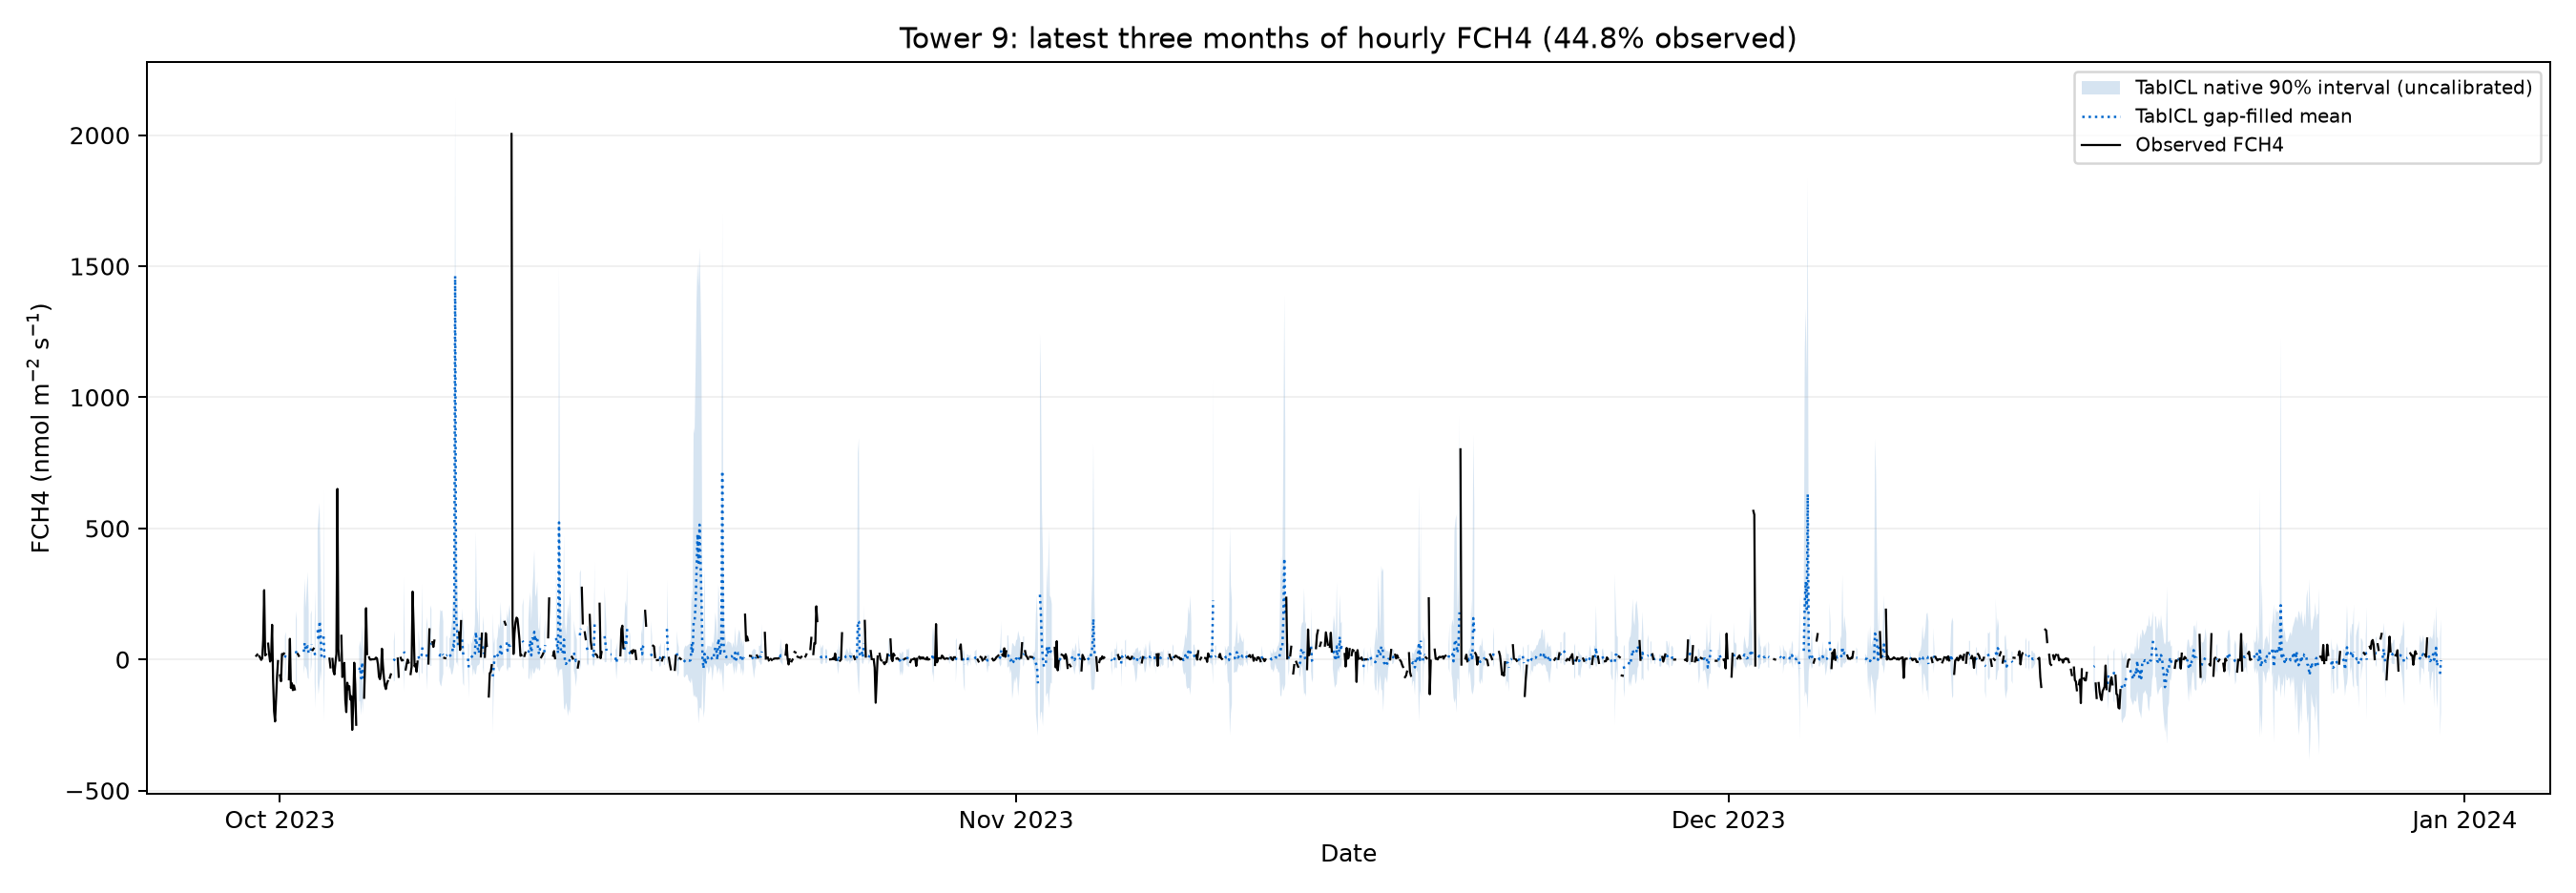
\includegraphics[width=\textwidth]{Figures/ch4_latest_tabicl_uq_hourly_T9_3month_example.png}
\caption{Three-month example of hourly FCH\textsubscript{4} reconstruction and
native uncertainty at T9. The figure shows QC-valid observations, the
TabICLv2 gap-filled mean and its uncalibrated native 90\% prediction interval
over the latest available three-month window, in which 44.8\% of the target
was observed. Corresponding T2 and T4 examples are provided in Appendix
Figure~\ref{fig:app_gf_tabicl_t2_t4}.}
\label{fig:gf_tabicl_hourly_examples}
\end{figure}

\FloatBarrier

Overall, TabICLv2 provides the strongest point reconstruction and is retained
as the gap-filling champion. Although calibrated coverage was close to the nominal target, the prediction 
intervals remained relatively wide, particularly at T9. Model identity and 
data-availability flags were therefore retained alongside the reconstructed 
FCH\textsubscript{4} series.

\FloatBarrier

%%%%%%%%%%%%%%%%%%%%%%%%%%%%%%%%%%%%%%%%%%%%%%%%%%%%%%%%%%%%%%%%%%%%%%%%%%%%%%%%
\chapter{Forecasting} \label{Chap5}

\section{Overview}

Forecasting extends beyond a fixed origin and therefore cannot use subsequent
FCH\textsubscript{4} observations as context. The experiments follow the five
365-day fixed-origin backtests defined in Chapter~\ref{ChapModels}. Supporting
variables over each evaluation period are treated as known, so the results
measure conditional methane-response forecasting rather than the additional
error involved in forecasting weather or management. Performance is evaluated
against QC-valid observed FCH\textsubscript{4}, not the reconstructed target
series produced in Chapter~\ref{Chap4}.

The benchmark models use different predictor subsets. To avoid repeating a
separate feature inventory for every model, Table~\ref{tab:fc_tabpfn_features}
reports the complete predictor frame used by the TabPFN model. Its best
configuration combines 52 daily environmental and
management drivers with five tower and time indicators. 

% \noindent\textbf{The best-performing forecasting model,}
% TabPFN and TabICL configuration averages three complementary
% TabPFN variants. The first uses all pre-origin observations with a spike
% correction: a classifier estimates whether FCH\textsubscript{4} exceeds the
% tower-specific 95th percentile, and 25\% of the predicted difference between
% spike and non-spike regressors is added to the base prediction. The other
% variants use the most recent 1,095 and 1,460 days, with the latter additionally
% applying tower-wise robust target normalisation. Equal-weight averaging reduces
% sensitivity to context length and spike-handling assumptions.

% NEW
\noindent\textbf{Best-performing forecasting model.}
The selected TabPFN and TabICLv2 models are equal-weight ensembles of three complementary
variants. The first uses all pre-origin observations with the following
probability-gated spike correction:
\[
\widehat{y}^{\,\mathrm{corr}}_t
=
\widehat{y}^{\,\mathrm{base}}_t
+
0.25\,p^{\mathrm{spike}}_t
\left[
\widehat{y}^{\,\mathrm{spike}}_t
-
\widehat{y}^{\,\mathrm{normal}}_t
\right]_{+},
\qquad [x]_{+}=\max(x,0).
\]
Here, \(p^{\mathrm{spike}}_t\) is the predicted probability of exceeding the
tower-specific, pre-origin 95th percentile. The probability gates the
correction, while the factor \(0.25\) retains only one quarter of the predicted
positive spike excess to limit overcorrection. The other variants use the most
recent 1,095 and 1,460 days, with the latter additionally applying tower-wise 
target normalisation. Equal-weight averaging reduces sensitivity to
context length and spike-handling assumptions.

\begin{table}[H]
\centering
\footnotesize
\renewcommand{\arraystretch}{1.12}
\begin{tabular*}{\textwidth}{@{\extracolsep{\fill}}
>{\raggedright\arraybackslash}p{0.21\textwidth}
>{\raggedright\arraybackslash}p{0.68\textwidth}
>{\centering\arraybackslash}p{0.05\textwidth}@{}}
\toprule
Predictor group & Included variables & Count \\
\midrule
Meteorology and surface energy &
Mean wind speed, friction velocity, mean/minimum/maximum air temperature,
VPD, shortwave radiation, net radiation, PPFD, soil heat flux,
precipitation and sine/cosine wind-direction components &
13 \\
\addlinespace[0.3em]

Soil state and history &
Current soil moisture and temperature; 7-, 14-, 21- and 28-day lags; and
7- and 14-day rolling means for both variables &
14 \\
\addlinespace[0.3em]

Seasonality &
Day-of-year sine and cosine encodings, growing-season indicator and winter
indicator &
4 \\
\addlinespace[0.3em]

Livestock and grazing &
Livestock-unit, cattle, sheep, lamb and total-liveweight densities, grazing
indicator and days since grazing &
7 \\
\addlinespace[0.3em]

Hydrology and land use &
Mean catchment flow, its 7-, 14-, 21- and 28-day lags and 7- and 14-day
rolling means, plus the arable-field indicator &
8 \\
\addlinespace[0.3em]

Management &
Fertilizer-N application rate and recency, together with the recency of lime
application, cultivation, cutting and manure application &
6 \\
\addlinespace[0.3em]

Tower and absolute time &
T2, T4 and T9 indicators, calendar year and days elapsed &
5 \\
\midrule
\textbf{Total} & \textbf{52 drivers and 5 tower/time indicators} & \textbf{57} \\
\bottomrule
\end{tabular*}
\caption{Complete daily predictor frame used by the TabPFN forecasting
configuration. Simpler benchmark models use model-specific subsets of these
variables.}
\label{tab:fc_tabpfn_features}
\end{table}

\section{Results}

\begin{table}[H]
\centering
\footnotesize
\resizebox{\textwidth}{!}{%
\begin{tabular}{@{}l >{\raggedright\arraybackslash}p{6.5cm} c c c c c@{}}
\toprule
Model & Key Configuration & MASE (seasonal mean) & MAE & RMSE & WAPE & Correlation \\
\midrule
\textbf{TabPFN} & 
  Equal-weight blend of all-history spike-corrected, 1,095-day and
  1,460-day TabPFN forecasts
& \textbf{0.6908} & \textbf{29.82} & 60.02 & \textbf{0.797} & \textbf{0.491} \\
TabICLv2 & 
  Equal-weight blend of all-history spike-corrected, 1,095-day and
  1,460-day TabICLv2 forecasts
& 0.7191 & 30.86 & 60.47 & 0.825 & 0.443 \\
\addlinespace[0.5em]
Ensemble & Equal-weighted mean of RF/XGBoost/LightGBM & 0.8020 & 34.06 & \textbf{52.25} & 0.991 & 0.379 \\
\addlinespace[0.5em]
XGBoost & \texttt{max\_depth}=2, \texttt{lr}=0.02, \texttt{n\_estimators}=400, \texttt{min\_child\_weight}=10 & 0.8038 & 34.02 & 52.30 & 0.988 & 0.364 \\
\addlinespace[0.5em]
TFT & \texttt{d\_model}=32, 4 attention heads, \texttt{dropout}=0.1, 28-day lookback & 0.8120 & 35.13 & 55.78 & 1.009 & 0.236 \\
\addlinespace[0.5em]
LightGBM & \texttt{num\_leaves}=7, \texttt{min\_child\_samples}=10, \texttt{lr}=0.02, \texttt{n\_estimators}=400 & 0.8166 & 34.81 & 52.83 & 1.014 & 0.371 \\
\addlinespace[0.5em]
Random Forest & \texttt{n\_estimators}=500, \texttt{min\_samples\_leaf}=10, \texttt{max\_features}=0.5 & 0.8411 & 35.17 & 52.91 & 1.045 & 0.380 \\
\addlinespace[0.5em]
SARIMAX & AIC-selected order ($p\in\{1,2\}$, $d=1$, $q\in\{0,1\}$, per tower/anchor) & 0.8741 & 36.11 & 54.35 & 1.082 & 0.348 \\
\addlinespace[0.5em]
LSTM & Hidden size 64, 28-day lookback & 0.9521 & 40.22 & 62.32 & 1.154 & 0.275 \\
\addlinespace[0.5em]
DLinear & Trend/seasonal decomposition, kernel=25, 28-day lookback & 1.1872 & 45.74 & 61.99 & 1.519 & 0.277 \\
\midrule
\textit{Seasonal Mean (baseline)} & & \textit{1.000} & 43.79 & 73.55 & 1.170 & $-0.004$ \\
\bottomrule
\end{tabular}%
}
\caption{Forecasting performance against QC-valid observed
FCH\textsubscript{4} across the evaluable 365-day fixed-origin backtests.
MASE is scaled against the pre-origin seasonal-mean reference, for which
MASE equals 1. Lower MASE, MAE, RMSE and WAPE indicate better performance, whereas
higher correlation is preferable.}
\label{tab:fc_model_comparison}
\end{table}

Table~\ref{tab:fc_model_comparison} shows that TabPFN achieved the strongest
overall forecasting performance, recording the lowest MASE (0.691), MAE
(29.82) and WAPE (0.797), together with the highest correlation (0.491).
The conventional ensemble achieved the lowest RMSE (52.25). TabICLv2 ranked
second by MASE at 0.719. The tree-based and ensemble
models formed the next performance group, whereas LSTM and DLinear were the
weakest configurations. DLinear was the only model with a MASE above 1,
indicating worse absolute error than the seasonal-mean reference.

\begin{figure}[htbp]
\centering
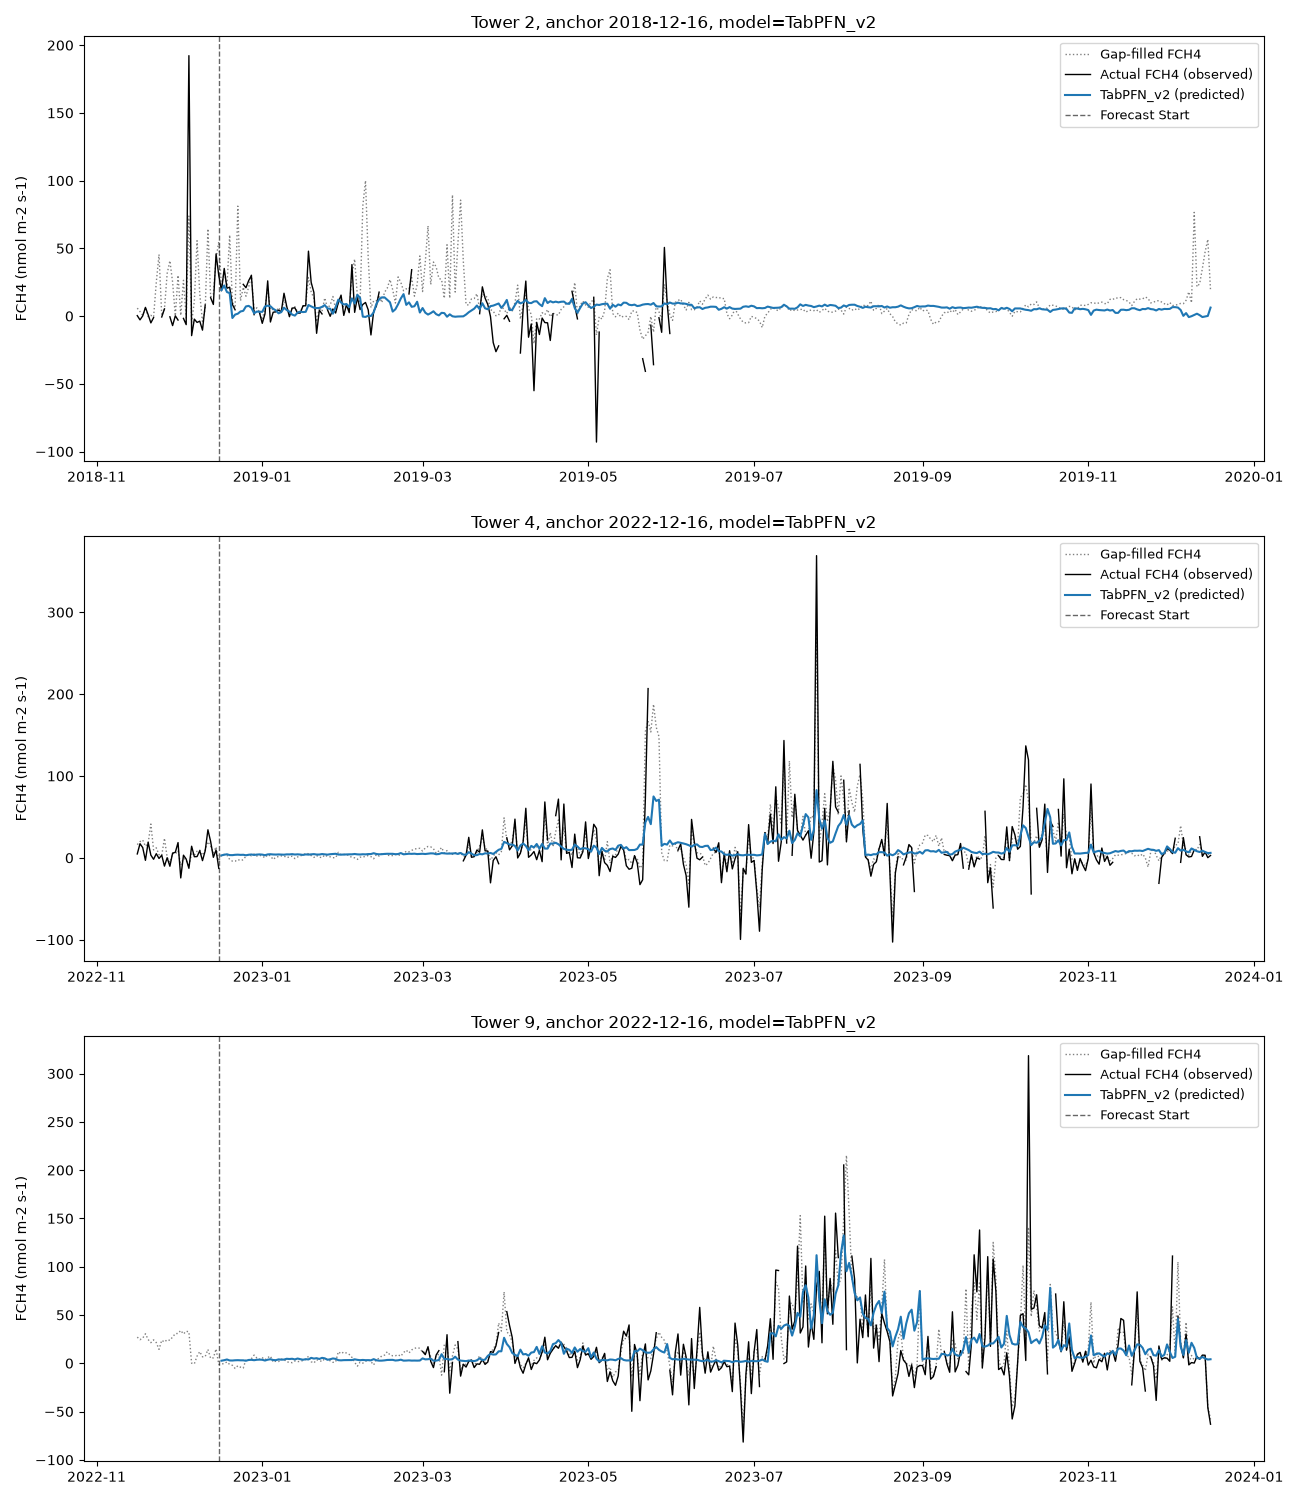
\includegraphics[width=0.85\textwidth]{Figures/ch5_champion_3towers.png}
\caption{Representative 365-day conditional forecasts from the TabPFN
model at T2, T4 and T9. The dashed vertical line marks the forecast origin;
blue lines show predictions, solid black lines show observed
FCH\textsubscript{4}, and dotted grey lines show the gap-filled series for
context.}
\label{fig:fc_champion_three_towers}
\end{figure}

\FloatBarrier

\subsection{Spike vs.\ Non-Spike Performance} \label{fc:spike}

The aggregate results conceal substantial differences between ordinary and
high-flux periods. Table~\ref{tab:fc_spike_performance} separates the
spike and non-spike observations for the TabPFN model using tower-specific
thresholds estimated exclusively from observations preceding each forecast
origin.

\begin{table}[htbp]
\centering
\footnotesize
\begin{tabular}{lcc}
\toprule
Metric & Non-spike ($n=1{,}997$) & Spike ($n=130$) \\
\midrule
MASE & 0.524 & 3.285 \\
MAE & 20.31 & 176.48 \\
RMSE & 30.01 & 210.12 \\
Bias (prediction $-$ observation) & $+1.48$ & \textbf{$-176.48$} \\
\bottomrule
\end{tabular}
\caption{Forecasting performance of the TabPFN model during non-spike and
spike periods. Spike thresholds are the tower-specific
95th percentiles estimated from pre-origin observed FCH\textsubscript{4}.}
\label{tab:fc_spike_performance}
\end{table}

Forecast errors are concentrated in the spike periods. Non-spike observations
achieved a MASE of 0.524 and MAE of 20.31, whereas spike observations reached
a MASE of 3.285 and MAE of 176.48. Bias changed from only $+1.48$ during
non-spike periods to $-176.48$ during spikes, showing that the dominant failure
is severe underprediction of high-flux events. The temporal distribution of
the evaluated spike observations is shown in Appendix
Figure~\ref{fig:app_fc_spike_timing}.

\subsection{Interpretability} \label{fc:interp}

Figure~\ref{fig:fc_tabpfn_importance} shows the permutation-sensitivity ranking for the 
TabPFN model. Livestock-unit density, total-liveweight density and cattle density occupy 
the first three positions, followed by grazing status; the remaining environmental and 
management variables have substantially smaller effects. The tower-specific rankings in 
Appendix Figure~\ref{fig:app_fc_importance_by_tower} show that this pattern is strongest 
at T4 and T9, whereas T2 relies primarily on environmental and management variables. 
Appendix Figure~\ref{fig:app_fc_importance_species} further separates the livestock 
related sensitivity by animal type.

\begin{figure}[H]
    \centering
    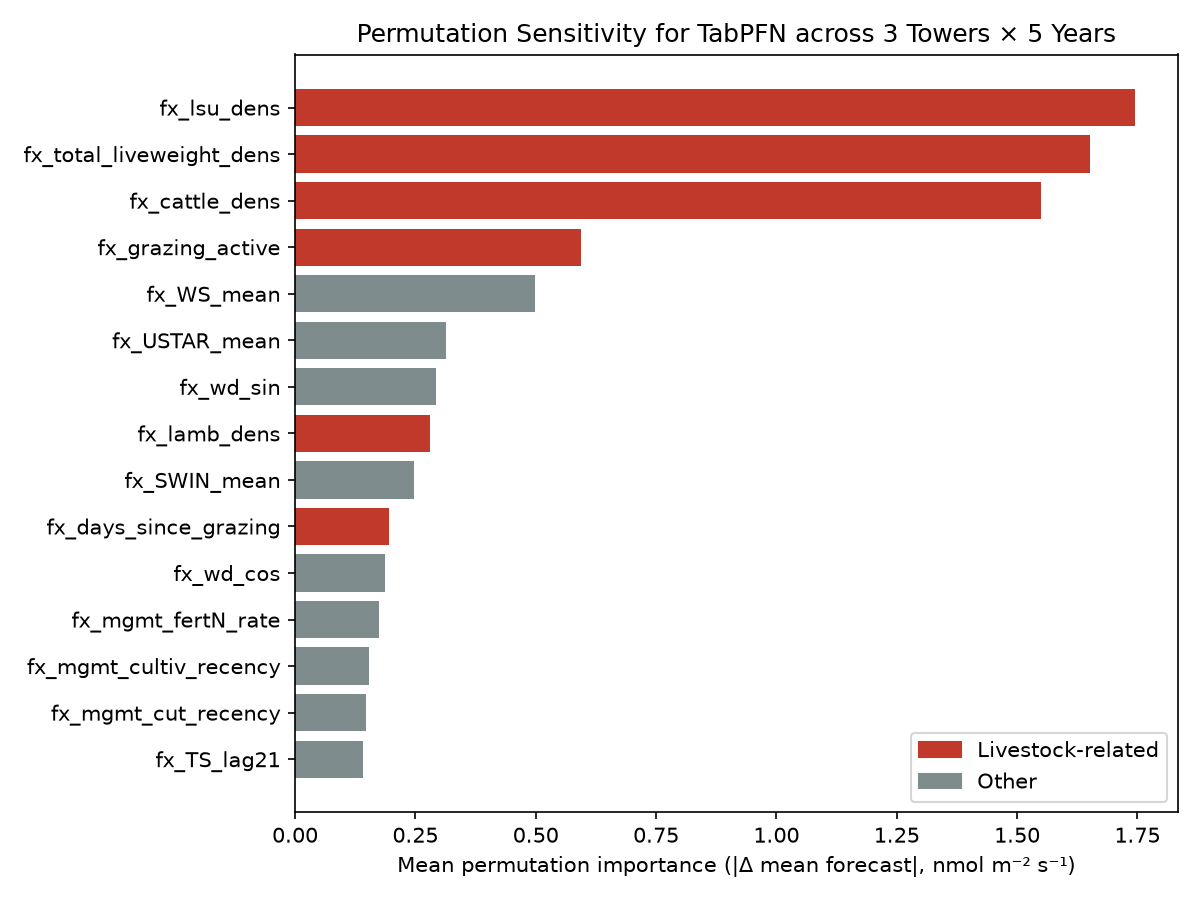
\includegraphics[width=0.8\textwidth]{Figures/ch5_tabpfn_permutation_sensitivity_overall.png}
    \caption{Permutation sensitivity of the TabPFN model, averaged across T2, T4 and T9 and five forecast origins. Each bar shows the absolute change in the mean forecast after shuffling one predictor within a tower; livestock-related variables are highlighted in red.}
    \label{fig:fc_tabpfn_importance}
\end{figure}

\subsection{Uncertainty Quantification}

Table~\ref{tab:fc_uq_by_tower} compares the raw and CQR-calibrated 90\%
prediction intervals for the TabPFN model. At T4 and T9, CQR reduced MPIW
while shifting the mild raw overcoverage to modest undercoverage: PICP changed
from 0.929 to 0.867 at T4 and from 0.928 to 0.871 at T9. T2 exhibited
substantial raw undercoverage, but its sparse
observed targets were insufficient to construct the leave-one-origin-out
calibration set. Figure~\ref{fig:fc_cqr_t4} illustrates the CQR interval
defined in Chapter~\ref{ChapModels} for T4; the corresponding T9 result is
provided in Appendix Figure~\ref{fig:app_fc_cqr_t9}. Appendix
Figure~\ref{fig:app_fc_uq_t2_raw} instead shows T2's uncalibrated raw interval.

\begin{table}[H]
\centering
\footnotesize
\begin{tabular}{lcccc}
\toprule
& \multicolumn{2}{c}{PICP} & \multicolumn{2}{c}{MPIW} \\
\cmidrule(lr){2-3}\cmidrule(lr){4-5}
Tower & Raw & CQR & Raw & CQR \\
\midrule
T2 & 0.726 & -- & 86.04 & -- \\
T4 & 0.929 & 0.867 & 187.13 & 178.14 \\
T9 & 0.928 & 0.871 & 192.84 & 186.89 \\
\bottomrule
\end{tabular}
\caption{Raw and CQR-calibrated 90\% prediction-interval performance for the
TabPFN model. PICP is the empirical
coverage proportion and MPIW is reported in
$\mathrm{nmol\,m^{-2}\,s^{-1}}$. CQR values are unavailable for T2
because too few observed targets remained to construct its calibration set.}
\label{tab:fc_uq_by_tower}
\end{table}

\begin{figure}[H]
\centering
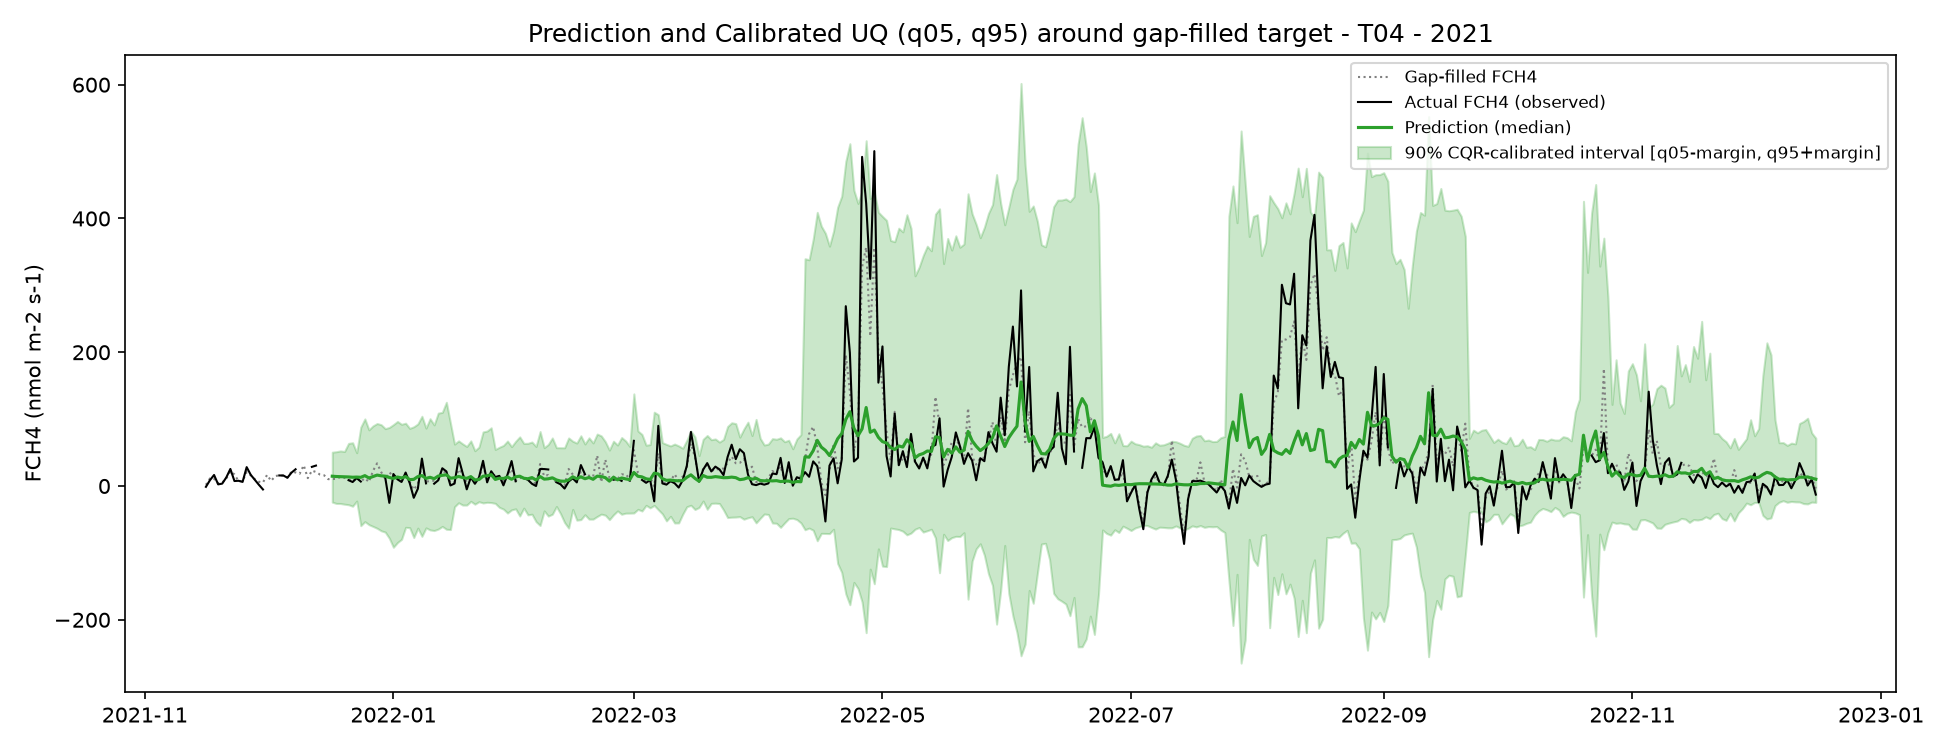
\includegraphics[width=\textwidth]{Figures/cqr_gallery/ch5_cqr_forecast_T04_2021.png}
\caption{Representative 365-day TabPFN forecast at T4 from the 2021 forecast
origin. The green line is the median forecast, the black line shows available
observations, the dotted line provides the gap-filled series as context, and
the shaded region is the 90\% CQR-calibrated prediction interval across the
complete forecast horizon. The corresponding T9 result is provided in Appendix
Figure~\ref{fig:app_fc_cqr_t9}.}
\label{fig:fc_cqr_t4}
\end{figure}

Overall, TabPFN achieved the strongest average forecasting performance, but
its errors remained concentrated during high-flux periods. Livestock-related
variables dominated its sensitivity at T4 and T9, while CQR produced modest
undercoverage and could not be applied at T2. These findings show that reliable
long-horizon forecasting remains constrained by abrupt methane dynamics and
sparse observations.

%%%%%%%%%%%%%%%%%%%%%%%%%%%%%%%%%%%%%%%%%%%%%%%%%%%%%%%%%%%%%%%%%%%%%%%%%%%%%%%%
\chapter{Scenario Projection} \label{Chap6}
\section{CMIP6-Derived Climate Scenarios}

% Future weather conditions were obtained from the transient climate dataset developed by \cite{semenov2025transient}. The dataset uses the LARS-WG 8.0 stochastic weather 
% generator to downscale projections from five CMIP6 Global Climate Models for representative locations across Great Britain, including North Wyke. It provides daily 
% minimum and maximum air temperature, precipitation and solar radiation from 2020 to 2090. This study uses the North Wyke simulations under two emissions pathways: the 
% intermediate SSP2-4.5 pathway and the very-high-emissions SSP5-8.5 pathway. Although the source dataset extends to 2090, the present analysis is restricted to 2050.

% The source dataset contains 100 stochastic realisations for each GCM--SSP combination. To retain variation between climate models while keeping the scenario experiment 
% computationally tractable, ten realisations were selected from each of the five GCMs. This produced 50 climate trajectories under each pathway and 100 trajectories 
% overall. Each trajectory contains four directly simulated variables: daily minimum temperature, maximum temperature, precipitation and solar radiation.

% These data differ substantially from the historical NWFP dataset used to develop the forecasting model. The NWFP data comprise tower- and catchment-level observations 
% derived from multiple monitoring systems, whereas the simulated climate data provide site-level daily weather trajectories shared across the three towers. They do not 
% contain FCH\textsubscript{4}, soil conditions, hydrological measurements, livestock records or field-management events. Consequently, the scenario model was restricted to 
% predictors that could either be obtained directly from the climate simulations or reconstructed consistently from the historical record.

% \begin{table}[htbp]
% \centering
% \small
% \renewcommand{\arraystretch}{1.15}
% \begin{tabularx}{\textwidth}{lXX}
% \toprule
% Property & Historical NWFP data & Simulated climate data \\
% \midrule
% Data source
% & Instrumental observations
% & LARS-WG simulations derived from five CMIP6 GCMs \\

% Temporal resolution
% & Hourly observations aggregated to daily values
% & Daily simulations \\

% Spatial representation
% & Tower- and catchment-specific
% & Site-level North Wyke climate \\

% Study period
% & Historical record ending in 2024
% & Future trajectories extending to 2050 \\

% Climate pathways
% & Not applicable
% & SSP2-4.5 and SSP5-8.5 \\

% Available variables
% & Meteorological, soil, hydrological, livestock, management and flux variables
% & Minimum temperature, maximum temperature, precipitation and solar radiation \\

% FCH\textsubscript{4}
% & Observed or gap-filled target
% & Not available; projected by the model \\
% \bottomrule
% \end{tabularx}
% \caption{Comparison between the historical NWFP observations and the simulated climate data used for scenario projection.}
% \label{tab:historical_scenario_comparison}
% \end{table}

% Before constructing the scenario predictor frames, the four simulated climate variables were standardised against the local NWFP climate record. Because the climate 
% trajectories represent the North Wyke site rather than individual tower locations, Tower~4 was used as the common observational reference owing to its comparatively 
% complete meteorological record. Separate correction factors were estimated for each GCM using its near-term SSP2-4.5 simulations from 2020--2030.

% Additive offsets were applied to minimum and maximum temperature, while multiplicative factors were applied to precipitation and solar radiation. The latter preserves 
% non-negative values and is more appropriate for ratio-scale variables. The resulting correction for each GCM was applied unchanged to both SSP2-4.5 and SSP5-8.5. This 
% aligned the simulated variables with the local climate baseline without removing the relative differences between GCMs or emissions pathways.

% The corrected variables were subsequently mapped to the forecasting data structure. Mean air temperature was calculated from the corrected daily minimum and maximum 
% temperatures, precipitation was retained as a daily total, and solar radiation was converted from MJ\,m\textsuperscript{-2}\,day\textsuperscript{-1} to mean 
% W\,m\textsuperscript{-2}. Calendar and historically derived farm-management predictors were then added to form the scenario-compatible input dataset.

Future weather conditions were obtained from the transient climate dataset developed by \cite{semenov2025transient}. It provides daily simulations of minimum and maximum air temperature, precipitation
and solar radiation for North Wyke from 2020 to 2090, generated using five CMIP6 Global Climate Models. This study selected ten realisations per GCM under SSP2-4.5 and SSP5-8.5, producing 100 climate
trajectories, and restricted the projection horizon to 2050.

Unlike the historical NWFP data, these simulations provide site-level daily weather rather than tower- and catchment-specific observations. They contain neither FCH\textsubscript{4} nor the soil,
hydrological, livestock and management measurements available historically. The scenario model was therefore restricted to predictors that could be obtained from the climate simulations or reconstructed
consistently from the NWFP record. Variables unavailable from CMIP6 were reconstructed from historical NWFP
  seasonality. Livestock densities were represented using tower-specific
  day-of-year seasonal mean, while grazing and fertiliser variables were derived
  from historical presence and event patterns. These profiles were repeated
  across future years and modified according to each scenario.

The four simulated climate variables were bias-corrected against the local NWFP record using Tower~4 as the common reference. Per-GCM correction factors were estimated from the 2020--2030 SSP2-4.5
simulations: additive offsets were applied to minimum and maximum temperature, while multiplicative factors were applied to precipitation and solar radiation. The same corrections were applied under both
pathways to preserve their relative differences. Mean temperature was subsequently derived from the corrected minimum and maximum values, and solar radiation was converted from
MJ\,m\textsuperscript{-2}\,day\textsuperscript{-1} to W\,m\textsuperscript{-2}.

Table~\ref{tab:climate_standardisation} reports the resulting correction factors. Raw simulations were cooler than the local record by 1.81--2.71$^\circ$C for daily minimum temperature and
2.60--3.56$^\circ$C for daily maximum temperature. Solar radiation required a modest upward adjustment of 3.4--8.3\%, whereas precipitation was reduced to 22.5--24.0\% of its raw value, indicating that
the uncorrected simulations were approximately 4.2--4.4 times wetter than the NWFP reference.

\begin{table}[htbp]
\centering
\small
\renewcommand{\arraystretch}{1.1}
\begin{tabular}{lrrrr}
\toprule
GCM & $\Delta T_{\min}$ ($^\circ$C) & $\Delta T_{\max}$ ($^\circ$C) &
SWIN ratio & Precipitation ratio \\
\midrule
ACCESS-ESM1-5   & 1.81 & 2.60 & 1.034 & 0.225 \\
CNRM-CM6-1      & 2.26 & 3.09 & 1.083 & 0.229 \\
HadGEM3-GC31-LL & 1.97 & 2.79 & 1.044 & 0.236 \\
MPI-ESM1-2-LR   & 2.71 & 3.56 & 1.060 & 0.226 \\
MRI-ESM2-0      & 2.29 & 3.03 & 1.043 & 0.240 \\
\bottomrule
\end{tabular}
\caption{Per-GCM correction factors used to standardise the simulated climate variables against the Tower~4 NWFP reference. Temperature offsets were added to raw simulated values; solar-radiation and
precipitation ratios were multiplied by raw simulated values.}
\label{tab:climate_standardisation}
\end{table}

\section{Results}

\subsection{Less Informed Model Creation}

This chapter's scenario model uses this dissertation's best forecasting model but restricted to
the 13 features that CMIP6 climate scenario can actually supply (climate drivers, calendar
encodings, livestock density, management practices) rather than the full
52-feature configuration used elsewhere in this dissertation (Chapter~\ref{Chap5}). This
restriction carries an accuracy cost that has been quantified:

\begin{table}[h]
\centering
\small
\renewcommand{\arraystretch}{1.1}
\begin{tabular}{lcc}
\toprule
Configuration & Feature count & MASE (seasonal mean) \\
\midrule
Full-feature model (Chapter~\ref{Chap5}) & 52 & 0.6908 \\
\textbf{Restricted model} & \textbf{13} & \textbf{0.7383} \\
\bottomrule
\end{tabular}
\caption{Accuracy cost of restricting the feature set to what CMIP6
climate scenario can supply. MASE scaled against the day-of-year seasonal mean baseline.}
\label{tab:sp_less_informed}
\end{table}

A restricted model is created using only the features available from the simulated climate
dataset. This model has a 6.9\% increase in MASE relative to the full-feature model (MASE
0.7383 vs.\ 0.6908), but remains sufficiently accurate for a projection task. This restricted
model is used for the inference task in the sections that follow.

% Restricting the feature set to only what a genuine climate scenario can supply carries a small,
% quantifiable accuracy cost: a real-anchor backtest found the direct-regression, per-tower,
% trend-augmented configuration recovers most of that cost (MASE 0.738, vs.\ 0.7405 for this
% dissertation's full-feature TabICLv2 configuration and 0.760 for a superseded one-shot engine) -- a
% $\sim$0.3\% cost rather than the superseded engine's 2.5\%. The trend covariate's own training range
% is $\sim$2.7$\times$ shorter than the horizon it is queried to (2050); a direct sanity check found it
% saturates to a bounded, plausible value rather than diverging when queried decades past its training
% maximum, unlike SARIMAX's known explosive extrapolation behaviour under a comparable stress test.

\subsection{Livestock Density Sensitivity}

Livestock density was varied along a four-level ladder: the historical baseline; half of the
baseline density; a policy-informed reference level of 2.5~LSU\,ha\textsuperscript{-1}; and each
tower's own historical maximum. The reference level is drawn from UK Countryside Stewardship
guidance for non-Severely Disadvantaged Area land \cite{defra2022stewardship}.

Reported scenario responses are mean percentage changes in annual predicted
FCH\textsubscript{4} relative to the matched baseline. They are averaged across the five GCMs and
ten selected realisations per GCM.

\begin{table}[h]
\centering
\small
\renewcommand{\arraystretch}{1.1}
\begin{tabular}{llrrr}
\toprule
SSP & Livestock level & T2 & T4 & T9 \\
\midrule
SSP2-4.5 & Half (0.5$\times$), all species & $-27.5\%$ & $-14.9\%$ & $-26.9\%$ \\
SSP2-4.5 & Government reference (2.5~LSU/ha) & $+4.6\%$ & $+0.9\%$ & $-2.6\%$ \\
SSP2-4.5 & Own historical maximum, all species & $+101.2\%$ & $+138.3\%$ & $+184.3\%$ \\
\midrule
SSP5-8.5 & Half (0.5$\times$), all species & $-27.2\%$ & $-15.0\%$ & $-26.9\%$ \\
SSP5-8.5 & Government reference (2.5~LSU/ha) & $+4.6\%$ & $+0.9\%$ & $-2.6\%$ \\
SSP5-8.5 & Own historical maximum, all species & $+99.7\%$ & $+138.1\%$ & $+181.9\%$ \\
\bottomrule
\end{tabular}
\caption{Mean percentage change in annual predicted FCH\textsubscript{4} relative to the matched
baseline livestock scenario, averaged across five GCMs and ten realisations per GCM.}
\label{tab:livestock_scenario_results}
\end{table}

  Livestock density produced the largest modelled response in the scenario grid.
  Halving stocking density reduced predicted annual FCH\textsubscript{4} by
  15--28\%, while raising it to each tower's historical maximum increased
  predicted flux by 100--184\%. The policy-informed reference level of
  2.5~LSU\,ha\textsuperscript{-1} was close to the historical baseline at T2 and
  T4, but below the baseline at T9, producing only small changes. Responses at
  each livestock level were similar under SSP2-4.5 and SSP5-8.5, indicating that
  the modelled sensitivity to livestock density was comparatively stable across
  the two climate pathways. Illustrative monthly trajectories are provided in
  Appendix Figures~\ref{fig:app_sp_livestock_trajectory_ssp245}
  and~\ref{fig:app_sp_livestock_trajectory_ssp585}.

% Tower 9's negative response at the literature-ceiling rung reflects that its real historical stocking
% density already exceeds that ceiling -- consistent with NWFP's identity as an intensively-managed
% research platform. At the "own historical maximum" rung, Tower 2's response ($+98.7\%$) is decisively
% weaker than Towers 4 or 9's ($+137.8\%$, $+182.9\%$), consistent with Tower 2's established
% livestock-blindness (Chapters~\ref{Chap4},~\ref{Chap5}) -- independently confirmed here for a fourth
% time, under a different model and climate driver source. In absolute annual generation terms, Tower
% 9's own-historical-max scenario reaches 260.7 kg~ha\textsuperscript{-1}~yr\textsuperscript{-1},
% nearly three times its baseline (27.7/72.4/92.2 kg~ha\textsuperscript{-1}~yr\textsuperscript{-1} at
% T2/T4/T9 respectively).

\FloatBarrier

\subsection{Grazing and Fertiliser Sensitivity}

\begin{table}[h]
\centering
\small
\renewcommand{\arraystretch}{1.1}
\begin{tabular}{llrrr}
\toprule
SSP & Intervention & T2 & T4 & T9 \\
\midrule
SSP2-4.5 & Extend grazing season by 4 weeks & $-3.8\%$ & $+19.9\%$ & $+20.0\%$ \\
SSP2-4.5 & Fertiliser frequency $+50\%$ & $-8.4\%$ & $\approx 0.0\%$ & $\approx 0.0\%$ \\
SSP2-4.5 & Fertiliser rate $+50\%$ & $-1.7\%$ & $-2.0\%$ & $\approx 0.0\%$ \\
\midrule
SSP5-8.5 & Extend grazing season by 4 weeks & $-3.7\%$ & $+19.9\%$ & $+19.9\%$ \\
SSP5-8.5 & Fertiliser frequency $+50\%$ & $-8.2\%$ & $-0.1\%$ & $\approx 0.0\%$ \\
SSP5-8.5 & Fertiliser rate $+50\%$ & $-1.7\%$ & $-2.0\%$ & $\approx 0.0\%$ \\
\bottomrule
\end{tabular}
\caption{Mean percentage change in annual predicted FCH\textsubscript{4} relative to the matched
historical scenario, averaged across five GCMs and ten realisations per GCM.}
\label{tab:management_scenario_results}
\end{table}

  Extending the grazing season by four weeks increased predicted annual
  FCH\textsubscript{4} by approximately 20\% at T4 and T9, whereas T2 produced a
  small negative response of approximately 4\%. Fertiliser interventions produced
  smaller and less consistent responses: increasing application frequency reduced
  predicted flux by approximately 8\% at T2 but had little effect at T4 and T9,
  while increasing the application rate changed predictions by no more than 2\%.
  The similarity between SSP2-4.5 and SSP5-8.5 indicates that these modelled
  management sensitivities were stable across the two climate pathways.
  Illustrative trajectories are provided in Appendix
  Figures~\ref{fig:app_sp_grazing_trajectory_ssp245}--%
  \ref{fig:app_sp_fertilizer_trajectory_ssp585}.

% Extending the grazing season by four weeks increases FCH\textsubscript{4} substantially at T4/T9
% ($\approx+20\%$), while T2's response is small and negative ($-3.7\%$ to $-3.8\%$), consistent
% with its muted livestock sensitivity. Fertiliser interventions are comparatively minor, changing
% predicted FCH\textsubscript{4} by at most 8.4\% (T2) and no more than 2\% at T4/T9. As with the
% livestock ladder, the SSP pathway makes almost no difference here -- management practice, not
% climate divergence, drives the response. Trajectories under both pathways are in Appendix
% Figures~\ref{fig:app_sp_grazing_trajectory_ssp245}--\ref{fig:app_sp_fertilizer_trajectory_ssp585}.

% Extending the grazing season produces a real, monotonic increase at Towers 4 and 9; Tower 2's small
% and sign-inconsistent response is consistent with its established livestock-blindness rather than a
% genuinely different underlying finding. Fertiliser perturbations produce a small, sign-inconsistent
% effect at every tower, consistent with this project's standing conclusion that fertiliser timing
% carries little independent signal once livestock density is already present. The SSP2-4.5 vs.\
% SSP5-8.5 pathway divergence is small relative to every management perturbation above throughout most
% of the horizon.

% \section{Limitations} \label{sp:lim}

% Three limitations apply specifically to this chapter's projections, beyond the general absence of
% ground truth. First, TabICLv2's extrapolation behaviour under genuine distribution shift (livestock
% density, climate drivers) has not been formally stress-tested to the standard applied to the
% production forecasting ensemble; the livestock-ladder sweep is a behavioural probe, not a controlled
% extrapolation test with any ground truth to check against. Second, no diagnostic available to this
% dissertation can detect a smooth-but-confidently-wrong extrapolation: historical PICP measures
% calibration only at real, historically-anchored points and cannot be computed for a genuine future
% scenario. Third, the CMIP6-vs-NWFP historical climate mismatch is corrected for but not eliminated as
% a source of residual uncertainty in every downstream scenario result.

%%%%%%%%%%%%%%%%%%%%%%%%%%%%%%%%%%%%%%%%%%%%%%%%%%%%%%%%%%%%%%%%%%%%%%%%%%%%%%%%
\chapter{Discussion and Conclusion} \label{Chap7}

\section{Main Findings}

\subsection{Overview of Model Performance} \label{sec:model_performance_overview}

\begin{itemize}
    \item \textbf{Gap-filling:} TabICLv2 is best (combined hourly $R^2=0.515$,
    Chapter~\ref{Chap4}), leading at T2/T4 and tying RF at T9. The two neural models nevertheless 
    underperformed compared to the leading tree-based and foundation-model approaches:
    bidirectional LSTM ($R^2=0.224$) and SAITS ($R^2=0.385$).
    \item \textbf{Forecasting:} TabPFN is best (MASE$=0.6908$, Chapter~\ref{Chap5}), while TabICLv2
    ranks second (MASE$=0.7191$). The weakest were again the locally trained deep-learning models:
    DLinear (MASE$=1.1872$, the only model worse than the seasonal-mean baseline) and LSTM (MASE$=0.9521$).
    \item \textbf{Tabular foundation models excel.} TabPFN and TabICLv2 are pretrained on
    millions of synthetic tabular datasets and predict via in-context learning, fitting no
    dataset-specific parameters \cite{hollmann2023tabpfn,hollmann2025tabpfn,qu2025tabicl,qu2026tabiclv2}.
    This prior-fitted-network approach is specifically effective on small, incomplete datasets
    \cite{hollmann2025tabpfn} and may provide an advantage on NWFP's severely incomplete record.
    \item \textbf{Deep learning does not perform best.} Locally trained neural architectures, 
    including LSTM, Bi-LSTM, DLinear and TFT train from scratch on NWFP's own incomplete 
    record, giving a small effective training-sample size. Off-the-shelf recurrent architectures 
    without dedicated missingness-handling tend only to match classical baselines (RF, SVM) on incomplete
    time series rather than exceed them \cite{che2018grud}. This is consistent with deep learning's broader
    failure to reliably beat tree-based methods on tabular data \cite{grinsztajn2022}.
    \item \textbf{Uncertainty quantification also favours the tabular foundation models.} In
    gap-filling, TabICLv2 matches QRF's calibrated coverage (PICP$=0.899$) with sharper intervals
    (MPIW $176.2$ vs.\ $183.5$, Chapter~\ref{Chap4}). In forecasting, TabPFN's raw intervals
    already sit close to nominal at T4/T9 (PICP$=0.929$/$0.928$) without extensive calibration --
    though not at Tower 2, where too few observations remain to calibrate at all
    (Chapter~\ref{Chap5}).
\end{itemize}

\subsection{Difficulty in Methane Flux Gap-Filling and Forecasting}

\begin{itemize}
    \item \textbf{Gap-filling fit remains modest despite the improved pipeline.} Even with
    enriched features and a tabular foundation model, the combined hourly $R^2$ reaches only
    0.515 (Chapter~\ref{Chap4}), a large improvement over MDS ($R^2=0.055$), but still a modest 
    absolute fit.
    \item \textbf{The livestock-dominant catchments are hardest to reconstruct.} T4 and T9, where
    livestock density dominates the FCH\textsubscript{4} signal, score \emph{below} the combined
    average ($R^2=0.429$/$0.430$), while T2, driven by a land-use transition, scores highest ($R^2=0.686$). 
    The catchments most central to this dissertation's finding are the ones it reconstructs least well.
    \item \textbf{Forecasting error is dominated by spikes.} Section~\ref{fc:spike} shows the
    champion's strong pooled MASE (0.6908) is earned almost entirely on ordinary days (non-spike
    MASE$=0.524$); on spike days it rises to 3.285, over six times worse and a clear loss against
    baseline. No feature in this project reliably predicts spike occurrence.
\end{itemize}

  \subsection{Scenario Sensitivity}

  Livestock density produced the largest modelled response among the tested
  scenarios, with historical-maximum stocking levels increasing predicted annual
  FCH\textsubscript{4} by 100--184\%. Extending grazing increased predictions by
  approximately 20\% at T4 and T9, whereas fertiliser interventions produced
  smaller and less consistent responses. These sensitivities were similar under
  SSP2-4.5 and SSP5-8.5, although they represent conditional model behaviour
  rather than validated causal effects.

\section{Limitations} \label{sec:limitations}

\begin{itemize}
    \item \textbf{Tower 2 is the weakest-conditioned data source at every pipeline stage.} Its
    QC-valid coverage is lowest of the three towers (92.0\% unavailable vs.\ 68.3\%/81.7\% at
    T4/T9, Chapter~\ref{Chap3}); it cannot support conformal calibration in forecasting
    (Chapter~\ref{Chap5}) due to data limitations.
    \item \textbf{Forecasting and scenario projection rely substantially on gap-filled variables.} Both
    build on Chapter~\ref{Chap4}'s reconstructed FCH\textsubscript{4} series, most of which is
    model-estimated, not observed (68.3--92.0\% of hours). Downstream results therefore partly
    reflect the gap-filling model's own behaviour.
    \item \textbf{UQ and scenario projection were not extended to the full model roster.}
    Gap-filling UQ covers only its top two models (QRF, TabICLv2, Chapter~\ref{Chap4});
    forecasting UQ covers only its champion (TabPFN, Chapter~\ref{Chap5}) -- extending further was
    not attempted given the compute cost. 
    \item \textbf{CMIP6 climate simulations do not match NWFP's own historical climate.} Raw air
    temperature runs 1.81--2.71$^\circ$C too cool and precipitation $\sim$4.2--4.4$\times$ too wet
    before correction (Chapter~\ref{Chap6}); the applied correction reduces but does not eliminate
    this as a residual uncertainty source.
    \item \textbf{Scenario projection has no ground truth to validate against.} No real
    CH\textsubscript{4} measurement exists for conditions that have never occurred at NWFP, and
    this dissertation makes no comparison against any process-based (mechanistic) methane model; 
    its results describe conditional model behaviour, not a validated forecast.
\end{itemize}

\section{Future Work}

\begin{itemize}
    \item \textbf{Rerun the experiment once extended Tower 2 data is released.} Tower 2's usable
    record is expected to grow soon: 2025 data has already been collected and is pending release.
    Rerunning once available would test whether Tower 2's results reflect a resolvable
    data-scarcity limitation (Section~\ref{sec:limitations}) rather than a persistent structural
    difference.
    \item \textbf{Livestock proximity to each tower's footprint as an additional gap-filling
    feature.} This dissertation's livestock-density feature is catchment-level, but an EC
    footprint shifts with wind direction, speed, and stability (Chapter~\ref{Chap2}), so
    catchment-level presence does not guarantee animals were within it. Proximity-weighted,
    footprint-aware livestock location via GPS or remote sensing could sharpen the single
    strongest predictor identified throughout this dissertation.
    \item \textbf{Benchmark tabular models against other eddy-covariance datasets.} This
    dissertation's finding that pretrained tabular foundation models outperform locally-trained
    alternatives under severe missingness (Section~\ref{sec:model_performance_overview}) was
    established at a single site. Testing the same roster against benchmarks such as FLUXNET-CH4
    \cite{irvin2021} would test whether this generalises. However, FLUXNET-CH4 predominantly
    covers wetlands and rice paddies rather than managed grasslands, so this would specifically test
    the pretrained-model and environmental-driver findings.
\end{itemize}

\section{Concluding Remarks}
Overall, this dissertation developed and evaluated an integrated framework for
methane-flux gap-filling, conditional forecasting and exploratory scenario
analysis at the North Wyke Farm Platform. Pretrained foundation models for
tabular data provided the strongest overall predictive performance, while
traditional tree-based methods generally outperformed locally trained neural
networks. Livestock-associated variables also formed the most consistent
influence across the forecasting and scenario experiments. These findings
remain constrained by substantial target missingness, poorly predicted
emission peaks and the absence of future ground truth, and the scenario
responses should not be interpreted as causal effects. Nevertheless, the
resulting benchmark provides a reproducible foundation for further methane
modelling at North Wyke and other managed grassland sites.

%%%%%%%%%%%%%%%%%%%%%%%%%%%%%%%%%%%%%%%%%%%%%%%%%%%%%%%%%%%%%%%%%%%%%%%%%%%%%%%%
% \chapter{Conclusion} \label{Chap8}

This project sets out to develop and evaluate
machine learning approaches for CH\textsubscript{4} gap-filling, forecasting, and scenario
projection at the North Wyke Farm Platform. All three have been delivered: a benchmarked
gap-filling pipeline (Chapter~\ref{Chap4}) improves combined hourly $R^2$ from 0.055 (MDS) to
0.515 (TabICLv2); a forecasting benchmark (Chapter~\ref{Chap5}), the first applied to this
ecosystem-scale signal at a managed temperate grassland, beats a seasonal-mean baseline by a wide
margin (MASE$=$0.6908, TabPFN); and a scenario-projection architecture (Chapter~\ref{Chap6})
produces distinguishable CH\textsubscript{4} responses to livestock, grazing, and climate
perturbations under CMIP6-derived trajectories to 2050.

Across the forecasting and scenario analyses, livestock-associated variables
emerged as the strongest recurring influence on predicted
CH\textsubscript{4} flux. Permutation importance placed livestock units, total
liveweight, and cattle density among the leading predictors at T4 and T9
(Chapter~\ref{Chap5}), while increasing livestock density produced the largest
scenario response: 100--184\% at each tower's historical maximum, compared
with at most 20\% for extended grazing and 8\% for fertiliser
(Chapter~\ref{Chap6}). Together, these results demonstrate a consistent
livestock-related signal, although they do not establish causality.

Tabular foundation models are the second recurring finding: TabICLv2 leads gap-filling and TabPFN
leads forecasting, both pretrained via in-context learning rather than fitting parameters to
NWFP's own severely incomplete record, a structural advantage as discussed in
Chapter~\ref{Chap7}.

It is worth being precise about what has, and has not, been shown. Gap-filling's improvement over
MDS is real but its absolute fit remains modest ($R^2=0.515$), and weakest specifically at the
livestock-dominant catchments this dissertation's central finding is about (Chapter~\ref{Chap7}).
Forecasting reliably beats a seasonal-mean baseline but not during CH\textsubscript{4}'s dominant
spike events (MASE 3.285 vs.\ 0.524 on ordinary days). Scenario projection produces
distinguishable, interpretable projections while carrying the limitation that no future scenario
can be checked against ground truth. 

Taken together, this dissertation delivers a benchmarked,
uncertainty-quantified foundation for CH\textsubscript{4} forecasting and scenario projection at a
managed UK grassland site that did not previously exist in the literature.

%%%%%%%%%%%%%%%%%%%%%%%%%%%%%%%%%%%%%%%%%%%%%%%%%%%%%%%%%%%%%%%%%%%%%%%%%%%%%%%%
\renewcommand{\bibname}{References}
\bibliographystyle{ieeetr}
%\bibliography{Bibliography.bib}
\bibliography{references.bib}
%%%%%%%%%%%%%%%%%%%%%%%%%%%%%%%%%%%%%%%%%%%%%%%%%%%%%%%%%%%%%%%%%%%%%%%%%%%%%%%%
% APPENDIX
\begin{appendices}
% \chapter{Project Plan}\label{app:projectplan}
% Aims/objectives, work plan and ethics review, per the module's interim
% submission (moved out of the main chapter sequence, matching the
% appendix convention used in comparable UCL dissertations).

% \chapter{Supplementary Experiments}\label{app:supplementary}
% Compressed ablation/negative-result log (one line + finding each,
% pointing to the DECISIONS.md decision ID) for experiments that inform
% Chapters \ref{Chap4}-\ref{Chap6} but are not needed in the main text:
% e.g. target transforms, hurdle-model diagnostics, monthly-downscale,
% CV- vs. rollout-based hyperparameter tuning, SAITS, SVM.

% These appendices collect supplementary figures and tables referenced from
% the main text but not reproduced there, grouped by the chapter they support.

\chapter{Data}
\label{app:data-dictionary}

The downloaded raw-data directory contains 186 annual CSV files from 26 logical dataset families.
The tables below document the EC variables and project-derived features used by the modelling
pipeline. The annual files are not perfectly schema-uniform: the 2017 greenhouse-gas
file has a malformed header containing appended unit fields, subsequent greenhouse-gas files place
units in a separate first data row, and the environmental-measurement schema decreases from 718 to
694 columns from 2022 as phosphorus streams for several catchments disappear. Annual query windows
also overlap at some boundary timestamps. Compilation therefore removes duplicated timestamps and
normalises the time index before hourly aggregation. The greenhouse-gas record ends on 1 January
2024, so its substantive observations cover 2017--2023. Later records are available for environmental,
livestock and management sources, but not for EC fluxes.

{
\scriptsize
\setlength{\tabcolsep}{2pt}
\renewcommand{\arraystretch}{1.14}
\setlength\LTleft{0pt}
\setlength\LTright{0pt}
\begin{longtable}{p{2.7cm}p{4.5cm}p{2.5cm}p{4.8cm}}
\caption{Complete base-variable dictionary for the raw eddy-covariance, biomet and turbulence files. Each listed base variable is repeated for Towers 2, 4 and 9. Definitions, units and native resolution follow the NWFP EC greenhouse-gas guide \cite{olde2023ec}; treatment and analytical role describe processing in this project. Tower identifiers and repeated suffixes are omitted for readability.}
\label{tab:ch3_ec_dictionary}\\
\toprule
Variable & Meaning & Unit and resolution & Treatment and analytical role \\
\midrule
\endfirsthead
\multicolumn{4}{l}{\tablename\ \thetable\ -- continued}\\
\toprule
Variable & Meaning & Unit and resolution & Treatment and analytical role \\
\midrule
\endhead
\midrule
\multicolumn{4}{r}{Continued on next page}\\
\endfoot
\bottomrule
\endlastfoot
\texttt{CO2} & Carbon-dioxide mole fraction measured by the gas analyser & mmol CO\textsubscript{2} mol$^{-1}$; 30 min & Available raw concentration; not retained as a direct model feature \\
\texttt{H2O} & Water-vapour mole fraction measured by the gas analyser & mmol H\textsubscript{2}O mol$^{-1}$; 30 min & Available raw concentration; not retained directly \\
\texttt{CH4} & Methane mole fraction measured by the gas analyser & nmol CH\textsubscript{4} mol$^{-1}$; 30 min & Distinct from ecosystem-scale methane flux; not retained directly \\
\texttt{TAU} and \texttt{TAU\_SSITC\_TEST} & Momentum flux and its steady-state/integral-turbulence quality class & kg m$^{-1}$ s$^{-2}$ and categorical; 30 min & Available turbulence output; not retained directly \\
\texttt{H} and \texttt{H\_SSITC\_TEST} & Sensible-heat flux and its quality class & W m$^{-2}$ and categorical; 30 min & Available energy-balance output; not retained directly \\
\texttt{LE} and \texttt{LE\_SSITC\_TEST} & Latent-heat flux and its quality class & W m$^{-2}$ and categorical; 30 min & Available energy-balance output; not retained directly \\
\texttt{FC} (FCO\textsubscript{2}) & Net ecosystem carbon-dioxide exchange & $\mu$mol CO\textsubscript{2} m$^{-2}$ s$^{-1}$; 30 min & Carbon-cycle predictor and partitioning input; values outside $[-100,100]$ are rejected \\
\texttt{FC\_SSITC\_TEST} & SSITC quality class for each carbon-dioxide-flux estimate & Categorical: 0 high, 1 medium, 2 low quality; 30 min & Classes 0 and 1 are retained before FCO\textsubscript{2} reconstruction \\
\texttt{FCH4} (FCH\textsubscript{4}) & Methane flux measured by eddy covariance & nmol CH\textsubscript{4} m$^{-2}$ s$^{-1}$; 30 min & Prediction target; classes 0 and 1 are retained and fluxes outside $[-500,3000]$ are treated as missing \\
\texttt{FCH4\_SSITC\_TEST} & SSITC quality class for each methane-flux estimate & Categorical: 0 high, 1 medium, 2 low quality; 30 min & Provider quality field used to screen the target \\
\texttt{WD} & Horizontal wind direction & degrees; 30 min & Converted to sine and cosine components when used in forecasting \\
\texttt{WS}/\texttt{WS\_MAX} & Mean and maximum horizontal wind speed & m s$^{-1}$; 30 min & Mean wind speed is retained; the maximum is available but not retained \\
\texttt{U/V/W\_SIGMA} & Standard deviations of the three wind components & m s$^{-1}$; 30 min & Available turbulence diagnostics; not retained directly \\
\texttt{USTAR} & Friction velocity representing atmospheric turbulence & m s$^{-1}$; 30 min & Predictor and diagnostic; values outside $[0,3]$ are removed, while the derived low-turbulence flag is not applied to FCH\textsubscript{4} \\
\texttt{MO\_LENGTH}/\texttt{ZL} & Monin--Obukhov length and dimensionless stability ratio $z/L$ & m and dimensionless; 30 min & Available atmospheric-stability diagnostics; not retained directly \\
\texttt{FETCH\_MAX}, \texttt{FETCH\_70/80/90} & Maximum fetch and distances containing 70, 80 and 90\% of the modelled footprint contribution & m; 30 min & Available footprint diagnostics; not retained as model features \\
\texttt{PA} & Atmospheric pressure & kPa; 30 min & Available meteorological variable; not retained directly \\
\texttt{RH\_0}/\texttt{RH\_1} & Relative humidity measured by the EC and biomet systems & \%; 30 min & Available but excluded from retained feature sets in favour of VPD \\
\texttt{TA\_0} (TA) & Air temperature & $^{\circ}$C; 30 min & Meteorological predictor and carbon-partitioning input; an external series is available \\
\texttt{VPD} & Vapour-pressure deficit, representing atmospheric moisture demand & hPa; 30 min & Retained predictor; a $[0,15]$\,hPa plausibility bound
  is applied before gap-filling to remove implausible
  outlier readings \\
\texttt{T\_SONIC} and sigma & Sonic temperature and its \texttt{T\_SONIC\_SIGMA} standard-deviation field & $^{\circ}$C; 30 min & Available sonic-anemometer outputs; not retained directly \\
\texttt{LWIN}/\texttt{LWOUT} & Incoming and outgoing long-wave radiation & W m$^{-2}$; 30 min & Available radiation components; not retained directly \\
\texttt{PPFD} & Incoming photosynthetic photon-flux density & $\mu$mol photons m$^{-2}$ s$^{-1}$; 30 min & Radiation and plant-activity predictor \\
\texttt{RN} & Net radiation at the land surface & W m$^{-2}$; 30 min & Surface-energy predictor \\
\texttt{SHF\_1/2/3} & Soil heat flux recorded by three plates & W m$^{-2}$; 30 min & Sensor 1 is retained in the base feature set; all three are averaged in selected forecasting configurations \\
\texttt{SWC\_1/2/3} & Volumetric soil-water content from three EC-biomet sensors & m$^{3}$ m$^{-3}$; 30 min & Available EC soil measurements; the adopted configuration instead uses catchment SMS observations \\
\texttt{SWIN}/\texttt{SWOUT} & Incoming and outgoing short-wave radiation & W m$^{-2}$; 30 min & Incoming radiation is retained; outgoing radiation is not retained directly \\
\texttt{TA\_1} & Secondary biomet air-temperature measurement & K; 30 min & Available raw measurement; not retained directly \\
\texttt{TS\_1/2/3} & Soil temperature from three EC-biomet sensors & K; 30 min & Sensor 1 at Tower 9 supplies the cross-tower proxy only in the EC-only configuration; adopted catchment SMS temperatures are in $^{\circ}$C \\
\end{longtable}
}

% Table disabled: detailed non-EC raw-input dictionary.
\iffalse
{
\scriptsize
\setlength{\tabcolsep}{2pt}
\renewcommand{\arraystretch}{1.14}
\setlength\LTleft{0pt}
\setlength\LTright{0pt}
\begin{longtable}{p{3.2cm}p{4.2cm}p{2.5cm}p{4.6cm}}
\caption{Dictionary of raw environmental, catchment, site-wide meteorological, livestock-count and field-event records. SMS definitions follow \cite{hawkins2023sms}, site-wide meteorology follows \cite{hawkins2023met}, hydrology and water quality follow the Data Guide \cite{hawkins2025}, and event definitions follow \cite{hawkins2023fieldevents}. Livestock-count descriptions are based on the downloaded files because a dedicated local livestock guide is unavailable.}
\label{tab:ch3_catchment_dictionary}\\
\toprule
Variable or record & Meaning & Unit and resolution & Treatment and analytical role \\
\midrule
\endfirsthead
\multicolumn{4}{l}{\tablename\ \thetable\ -- continued}\\
\toprule
Variable or record & Meaning & Unit and resolution & Treatment and analytical role \\
\midrule
\endhead
\midrule
\multicolumn{4}{r}{Continued on next page}\\
\endfoot
\bottomrule
\endlastfoot
Flume flow and pump status & Discharge derived from the instrumented catchment flume and the associated pump on/off state & L s$^{-1}$ and binary; 15 min & Flow is aggregated to hourly or daily means for extended experiments; pump status is not retained \\
Water temperature & Temperature measured in the flume and in the water-quality flow cell & $^{\circ}$C; 15 min & Available hydrological diagnostics; not retained in the base analytical feature set \\
Inorganic nitrogen chemistry & Nitrite plus nitrate, ammonia and ammonium concentrations & mg L$^{-1}$; 15 min & Available water-quality measurements; not retained in the base analytical feature set \\
Phosphorus chemistry & Total and orthophosphorus concentrations & mg L$^{-1}$; 15 min & Not retained; streams for Catchments 2, 3, 5 and 8 disappear from the downloaded schema from 2022 \\
Conductivity and dissolved oxygen & Electrical conductivity and percentage oxygen saturation & $\mu$S cm$^{-1}$ and \%; 15 min & Available water-quality measurements; not retained \\
pH, turbidity and fluorescent DOM & Acidity, optical turbidity and fluorescent dissolved organic matter & dimensionless, FNU and $\mu$g L$^{-1}$ QSU; 15 min & Available water-quality measurements; not retained \\
Catchment precipitation & Tipping-bucket precipitation recorded at the soil-moisture station; the gauge resolves 0.2 mm per tip & mm; 15 min & Aggregated hourly or to daily totals and matched only to the corresponding tower \\
Soil moisture at 10 cm & Volumetric soil-water content measured by capacitance at 10 cm & \%; 15 min & Aggregated to hourly means and used as a soil-condition predictor \\
Soil temperature at 15 cm & Soil temperature measured by the catchment soil-moisture station at 15 cm depth & $^{\circ}$C; 15 min & Aggregated to hourly means and used as a soil-condition predictor \\
Site precipitation & Precipitation measured by the dedicated site-wide meteorological station & mm; 15 min & External meteorological input; reported using a tipping bucket before 2015 and a weighing gauge thereafter \\
Site air temperature and RH & Air temperature and relative humidity measured by the dedicated meteorological station & $^{\circ}$C and \% RH; 15 min & Air temperature is adopted as an external input; relative humidity is available but not retained \\
Site wind speed and direction & Wind measured at 3 m height & km h$^{-1}$ and degrees; 15 min & Speed is divided by 3.6 before use; direction is available but the retained circular encoding uses EC wind \\
Site solar radiation & Incoming solar radiation measured by pyranometer & W m$^{-2}$; 15 min & Adopted external short-wave-radiation input \\
Provider \texttt{Quality} & Categorical validity assessment accompanying every environmental measurement series & Categorical; 15 min & Values include Acceptable, Not set, Outlier and Suspicious, with additional sensor-specific categories; these strings are currently discarded during numeric consolidation rather than applied as filters \\
Provider \texttt{Quality Last Modified} & Timestamp recording the most recent change to the corresponding quality assessment & Timestamp; 15 min & Retained in the raw files but discarded during numeric consolidation \\
Cattle, breeding-sheep and lamb counts & Numbers of each livestock class recorded at each catchment, shed and other listed location & head count; daily & The three \texttt{Animal\_location\_counts} families are expanded to the hourly index; Catchments 2, post-2013 Catchment 4 and 9 are selected \\
Event date and time fields & \texttt{Event\_Date}, entry/exit times and calculated time in field & Date, time and duration; event based & Establish the timing of a management record; date is used to construct recency features \\
Field and machinery fields & Field identifier, tractor, operator, and start, end and total tractor hours & Identifiers and hours; event based & Field identifiers are mapped to catchments; machinery metadata are not retained \\
Operation and application fields & \texttt{Field\_Operation} and \texttt{Application} descriptions & Categorical; event based & Raw records span fertiliser, pesticide, drainage, mowing, harvest, cultivation and other operations \\
Application quantity fields & Total application, units, application information, rate per hectare and batch number & Mixed units; event based & Used only where the operation and unit permit a defensible management feature \\
Product fields & Product name and manufacturer & Text; event based & Used by later corrected fertiliser processing to distinguish products and infer true nitrogen content \\
Derived management channels & Cutting, manure, fertiliser-classified, liming and cultivation histories classified from the raw event fields & Project-defined event categories & Cutting and manure recencies are retained in the pruned gap-filling set; the generic fertiliser classifier is not necessarily equivalent to confirmed nitrogen application \\
\end{longtable}
}
\fi

{
\scriptsize
\setlength{\tabcolsep}{2pt}
\renewcommand{\arraystretch}{1.14}
\setlength\LTleft{0pt}
\setlength\LTright{0pt}
\begin{longtable}{p{2.8cm}p{4.4cm}p{2.7cm}p{4.6cm}}
\caption{Dictionary of principal project-derived variables. These are not original NWFP portal columns: their definitions follow the repository's preprocessing and feature-construction code, while the underlying raw measurements use the guide-based definitions in the preceding tables.}
\label{tab:ch3_derived_dictionary}\\
\toprule
Derived variable & Meaning or derivation & Unit & Analytical role \\
\midrule
\endfirsthead
\multicolumn{4}{l}{\tablename\ \thetable\ -- continued}\\
\toprule
Derived variable & Meaning or derivation & Unit & Analytical role \\
\midrule
\endhead
\midrule
\multicolumn{4}{r}{Continued on next page}\\
\endfoot
\bottomrule
\endlastfoot
Gap-filled FCO\textsubscript{2} & QC-valid observations are retained; missing values are reconstructed separately for each tower using a meteorology-based random forest & $\mu$mol CO\textsubscript{2} m$^{-2}$ s$^{-1}$ & Environmental predictor and basis for GPP and Reco \\
GPP & Gross primary productivity from Reichstein/Lloyd--Taylor partitioning; $\max(\mathrm{Reco}-\mathrm{NEE},0)$ and zero at night & $\mu$mol CO\textsubscript{2} m$^{-2}$ s$^{-1}$ & Plant-productivity predictor \\
Reco & Ecosystem respiration from the Lloyd--Taylor temperature response using global $E_0$ and seven-day-block $R_{\mathrm{ref}}$ refitting & $\mu$mol CO\textsubscript{2} m$^{-2}$ s$^{-1}$ & Ecosystem-respiration predictor \\
LSU density & $(1.0N_{\mathrm{cattle}}+0.1N_{\mathrm{sheep}}+0.05N_{\mathrm{lamb}})/A$; the pipeline uses $A=6.65$ ha for Catchment 2 and $7.75$ ha for Catchments 4 and 9 & LSU ha$^{-1}$ & Standardised grazing-intensity predictor; the Catchment 2 constant represents its historical fenced area rather than its post-conversion cropped area \\
Grazing active & One when the summed livestock count is greater than zero; otherwise zero & Binary & Management-state predictor; the current implementation fills missing species counts with zero before calculating it \\
Current grazing-spell duration & Zero on non-grazing days; on grazing days, zero on the first day and incremented for each subsequent consecutive day & days & Run-length measure of the active grazing spell; despite its code name, it is not elapsed time since the last grazing event \\
Cutting recency & $\exp(-d_{\mathrm{cut}}/21)$ & Dimensionless $[0,1]$ & Retained management predictor \\
Manure recency & $\exp(-d_{\mathrm{manure}}/30)$ & Dimensionless $[0,1]$ & Retained management predictor \\
Hour sine and cosine & $\sin(2\pi h/24)$ and $\cos(2\pi h/24)$ & Dimensionless & Diurnal timing predictors \\
Day-of-year sine and cosine & $\sin(2\pi d/365)$ and $\cos(2\pi d/365)$ & Dimensionless & Seasonal timing predictors \\
Soil-moisture lags & Gap-filled soil moisture shifted by 168, 336, 504 and 672 hours & \% & One- to four-week environmental-memory predictors \\
Soil-temperature lags & Gap-filled soil temperature shifted by 168, 336, 504 and 672 hours & $^{\circ}$C for the adopted SMS configuration; K for the EC-only proxy & One- to four-week environmental-memory predictors \\
Three-sensor SHF mean & Arithmetic mean of SHF1, SHF2 and SHF3 & W m$^{-2}$ & Forecasting predictor in selected configurations \\
Wind-direction components & $\sin(\theta)$ and $\cos(\theta)$ for wind direction $\theta$ in radians & Dimensionless & Circular encoding that removes the discontinuity at $0^{\circ}/360^{\circ}$ \\
Tower indicators & One-hot variables \texttt{is\_t2}, \texttt{is\_t4} and \texttt{is\_t9} & Binary & Preserve tower identity in partially pooled models \\
\end{longtable}
}

% Table disabled: inventory of excluded variables and datasets.
\iffalse
{
\scriptsize
\setlength{\tabcolsep}{2pt}
\renewcommand{\arraystretch}{1.15}
\setlength\LTleft{0pt}
\setlength\LTright{0pt}
\begin{longtable}{p{3.5cm}p{3.0cm}p{8.0cm}}
\caption{Status of downloaded measurements, candidate variables and separately documented NWFP datasets not used directly in the base analytical feature set.}
\label{tab:ch3_excluded_dictionary}\\
\toprule
Available variable or dataset & Status & Rationale or subsequent treatment \\
\midrule
\endfirsthead
\multicolumn{3}{l}{\tablename\ \thetable\ -- continued}\\
\toprule
Available variable or dataset & Status & Rationale or subsequent treatment \\
\midrule
\endhead
\midrule
\multicolumn{3}{r}{Continued on next page}\\
\endfoot
\bottomrule
\endlastfoot
Relative humidity & Excluded from retained sets & VPD is retained as the atmospheric-moisture-demand variable \\
Raw wind direction & Transformed where used & Replaced by sine and cosine components to preserve circular continuity \\
Catchment flow & Excluded from base gap filler & Available to extended forecasting experiments examining hydrological history \\
Water-quality chemistry and hydrological diagnostics & Excluded from base analytical set & The raw measurement files contain nutrient chemistry, conductivity, dissolved oxygen, pH, turbidity, fluorescent DOM, water temperature and pump status in addition to flume flow \\
Provider environmental-quality fields & Discarded during consolidation & The current numeric conversion removes \texttt{Quality} and \texttt{Quality Last Modified}; this must not be interpreted as provider-QC filtering \\
Site-wide and non-local soil data & Excluded & Each tower uses only measurements from its corresponding catchment \\
GreenFeed animal-gas measurements \cite{demeofilho2023greenfeed} & Separate dataset; not downloaded or used & GreenFeed records individual-animal enteric CH\textsubscript{4} and CO\textsubscript{2} during voluntary feeding visits; no GreenFeed CSV is present in the consolidated raw-data directory, and it is distinct from tower-level EC flux and livestock-location counts \\
Feed-type and detailed field surveys & Downloaded but excluded from the base set & The raw directory includes feed type and botanical, grain, herbage, silage-cut and soil chemistry/physics surveys; these were not connected to the retained pipelines \\
Individual-animal basic, location, sales, weight and condition records & Downloaded but excluded from the base set & Daily catchment-level count tables provide the directly aligned grazing variables; later experimental use of individual-animal information is documented at first use \\
Fertiliser, liming and cultivation variables & Pruned from gap-filling set & Larger management sets were unstable; catchment-specific cutting and manure recency were retained \\
Site-wide management scopes & Pruned from gap-filling set & Catchment-specific event histories provide the spatially aligned representation \\
USTAR low-turbulence flag & Diagnostic only & Calculated but not applied directly to FCH\textsubscript{4} because methane low-turbulence filtering is not treated as an uncontested validity rule \\
\end{longtable}
}
\fi

The auxiliary-data calibration procedure referenced in
Section~\ref{sec:ch3_environmental_preparation} is reproduced in
Algorithm~\ref{alg:auxiliary-driver-gapfill}.

\begin{algorithm}[htbp]
\caption{Auxiliary-data gap filling of meteorological variables adapted from the NWFP EC processing report \cite{nwfp2022ecqc}}
\label{alg:auxiliary-driver-gapfill}
\begin{algorithmic}[1]

\Require Primary EC series $x_{1:T}$;
         auxiliary series $z_{1:T}$;
         timestamps $t_{1:T}$;
         variable name $v$
\Ensure Gap-filled series $\hat{x}_{1:T}$

\State $\hat{x} \gets x$

\Comment{Variable-specific quality control}
\If{$v = \mathrm{PA}$}
    \State Decompose $x$ using STL with hourly frequency
    \State Detect anomalies in the decomposition remainder
    \State Replace detected anomalies in $x$ with $\mathrm{NaN}$
\ElsIf{$v = \mathrm{LE}$}
    \State Replace the manually identified outlier with $\mathrm{NaN}$
\ElsIf{$v = \mathrm{TA}$}
    \State Convert the primary temperature to the units of the auxiliary series
\EndIf

\Comment{Variables replaced directly by auxiliary measurements}
\If{$v = \mathrm{SWC}$}
    \State $\hat{x} \gets z^{\mathrm{COSMOS},1}$
    \State \Return $\hat{x}_{1:T}$
\ElsIf{$v = \mathrm{TS}$}
    \State $\hat{x} \gets z^{\mathrm{COSMOS},2}$
    \State \Return $\hat{x}_{1:T}$
\EndIf

\Comment{Fit calibration model using paired observations}
\State $\mathcal{I}
    \gets
    \{t : x_t \neq \mathrm{NaN}
    \land z_t \neq \mathrm{NaN}\}$

\State Fit
\[
    x_t = \beta_0 + \beta_1 z_t + \varepsilon_t,
    \qquad t \in \mathcal{I}
\]

\Comment{Preserve measurements and fill missing values}
\For{$t \gets 1$ to $T$}
    \If{$x_t \neq \mathrm{NaN}$}
        \State $\hat{x}_t \gets x_t$
    \ElsIf{$z_t \neq \mathrm{NaN}$}
        \State $\hat{x}_t
        \gets \hat{\beta}_0 + \hat{\beta}_1 z_t$
    \Else
        \State $\hat{x}_t \gets \mathrm{NaN}$
    \EndIf
\EndFor

\State \Return $\hat{x}_{1:T}$

\end{algorithmic}
\end{algorithm}

\clearpage

\begin{figure}[p]
\centering
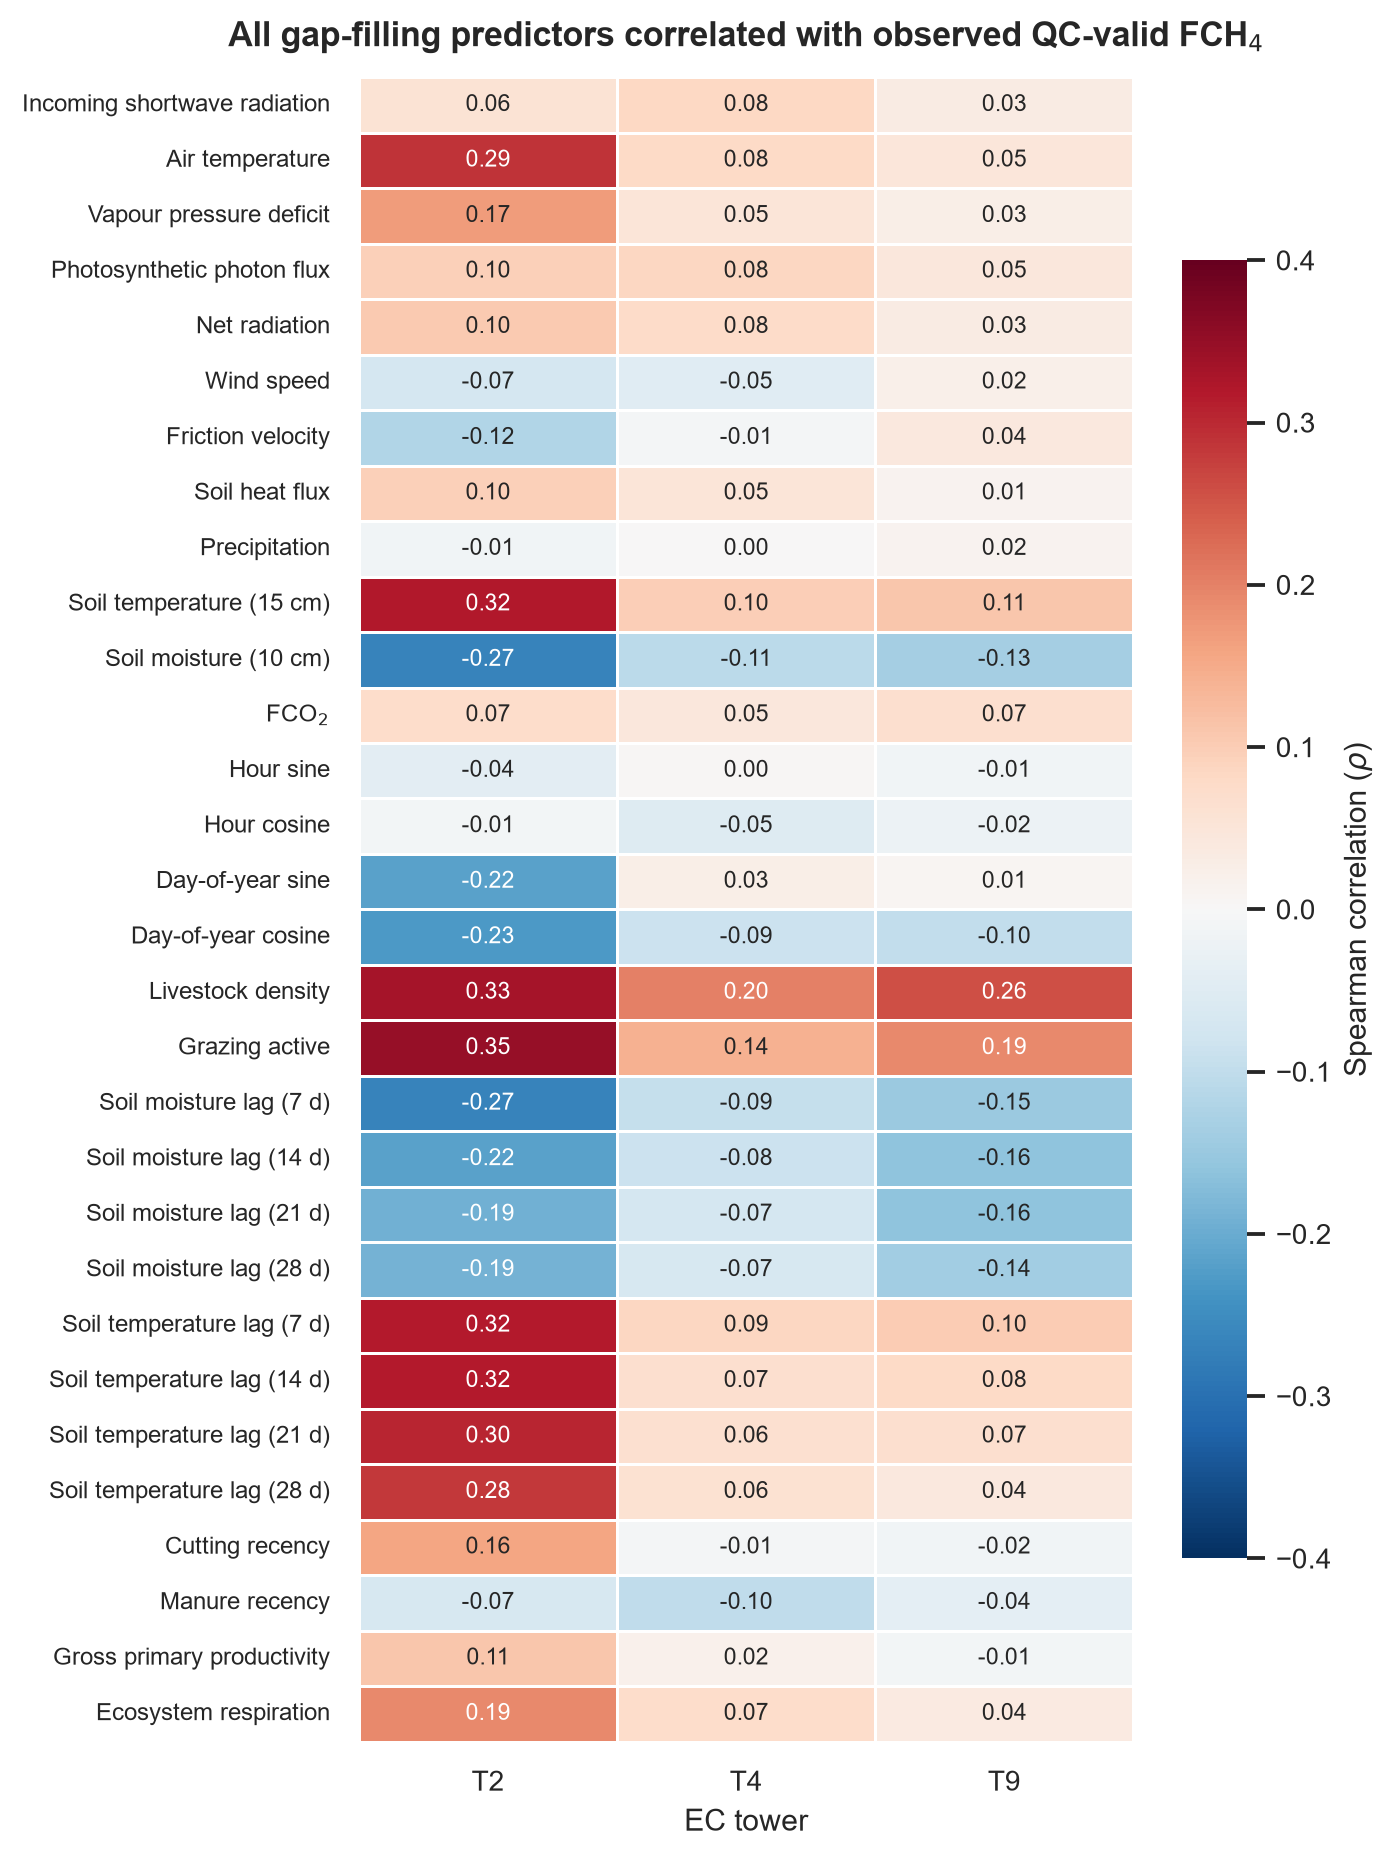
\includegraphics[width=0.82\textwidth]{Figures/ch3_fch4_target_correlations_full.png}
\caption{Complete matrix of tower-specific Spearman correlations between observed QC-valid
FCH\textsubscript{4} and all 30 predictors used by the gap-filling experiments. The reduced matrix
in Figure~\ref{fig:ch3_target_correlations} presents the union of the five largest absolute
correlations within each tower. These coefficients describe pairwise monotonic association and
should not be interpreted as causal effects or model-based feature importance.}
\label{fig:appendix_target_correlations_full}
\end{figure}

\begin{figure}[htbp]
\centering
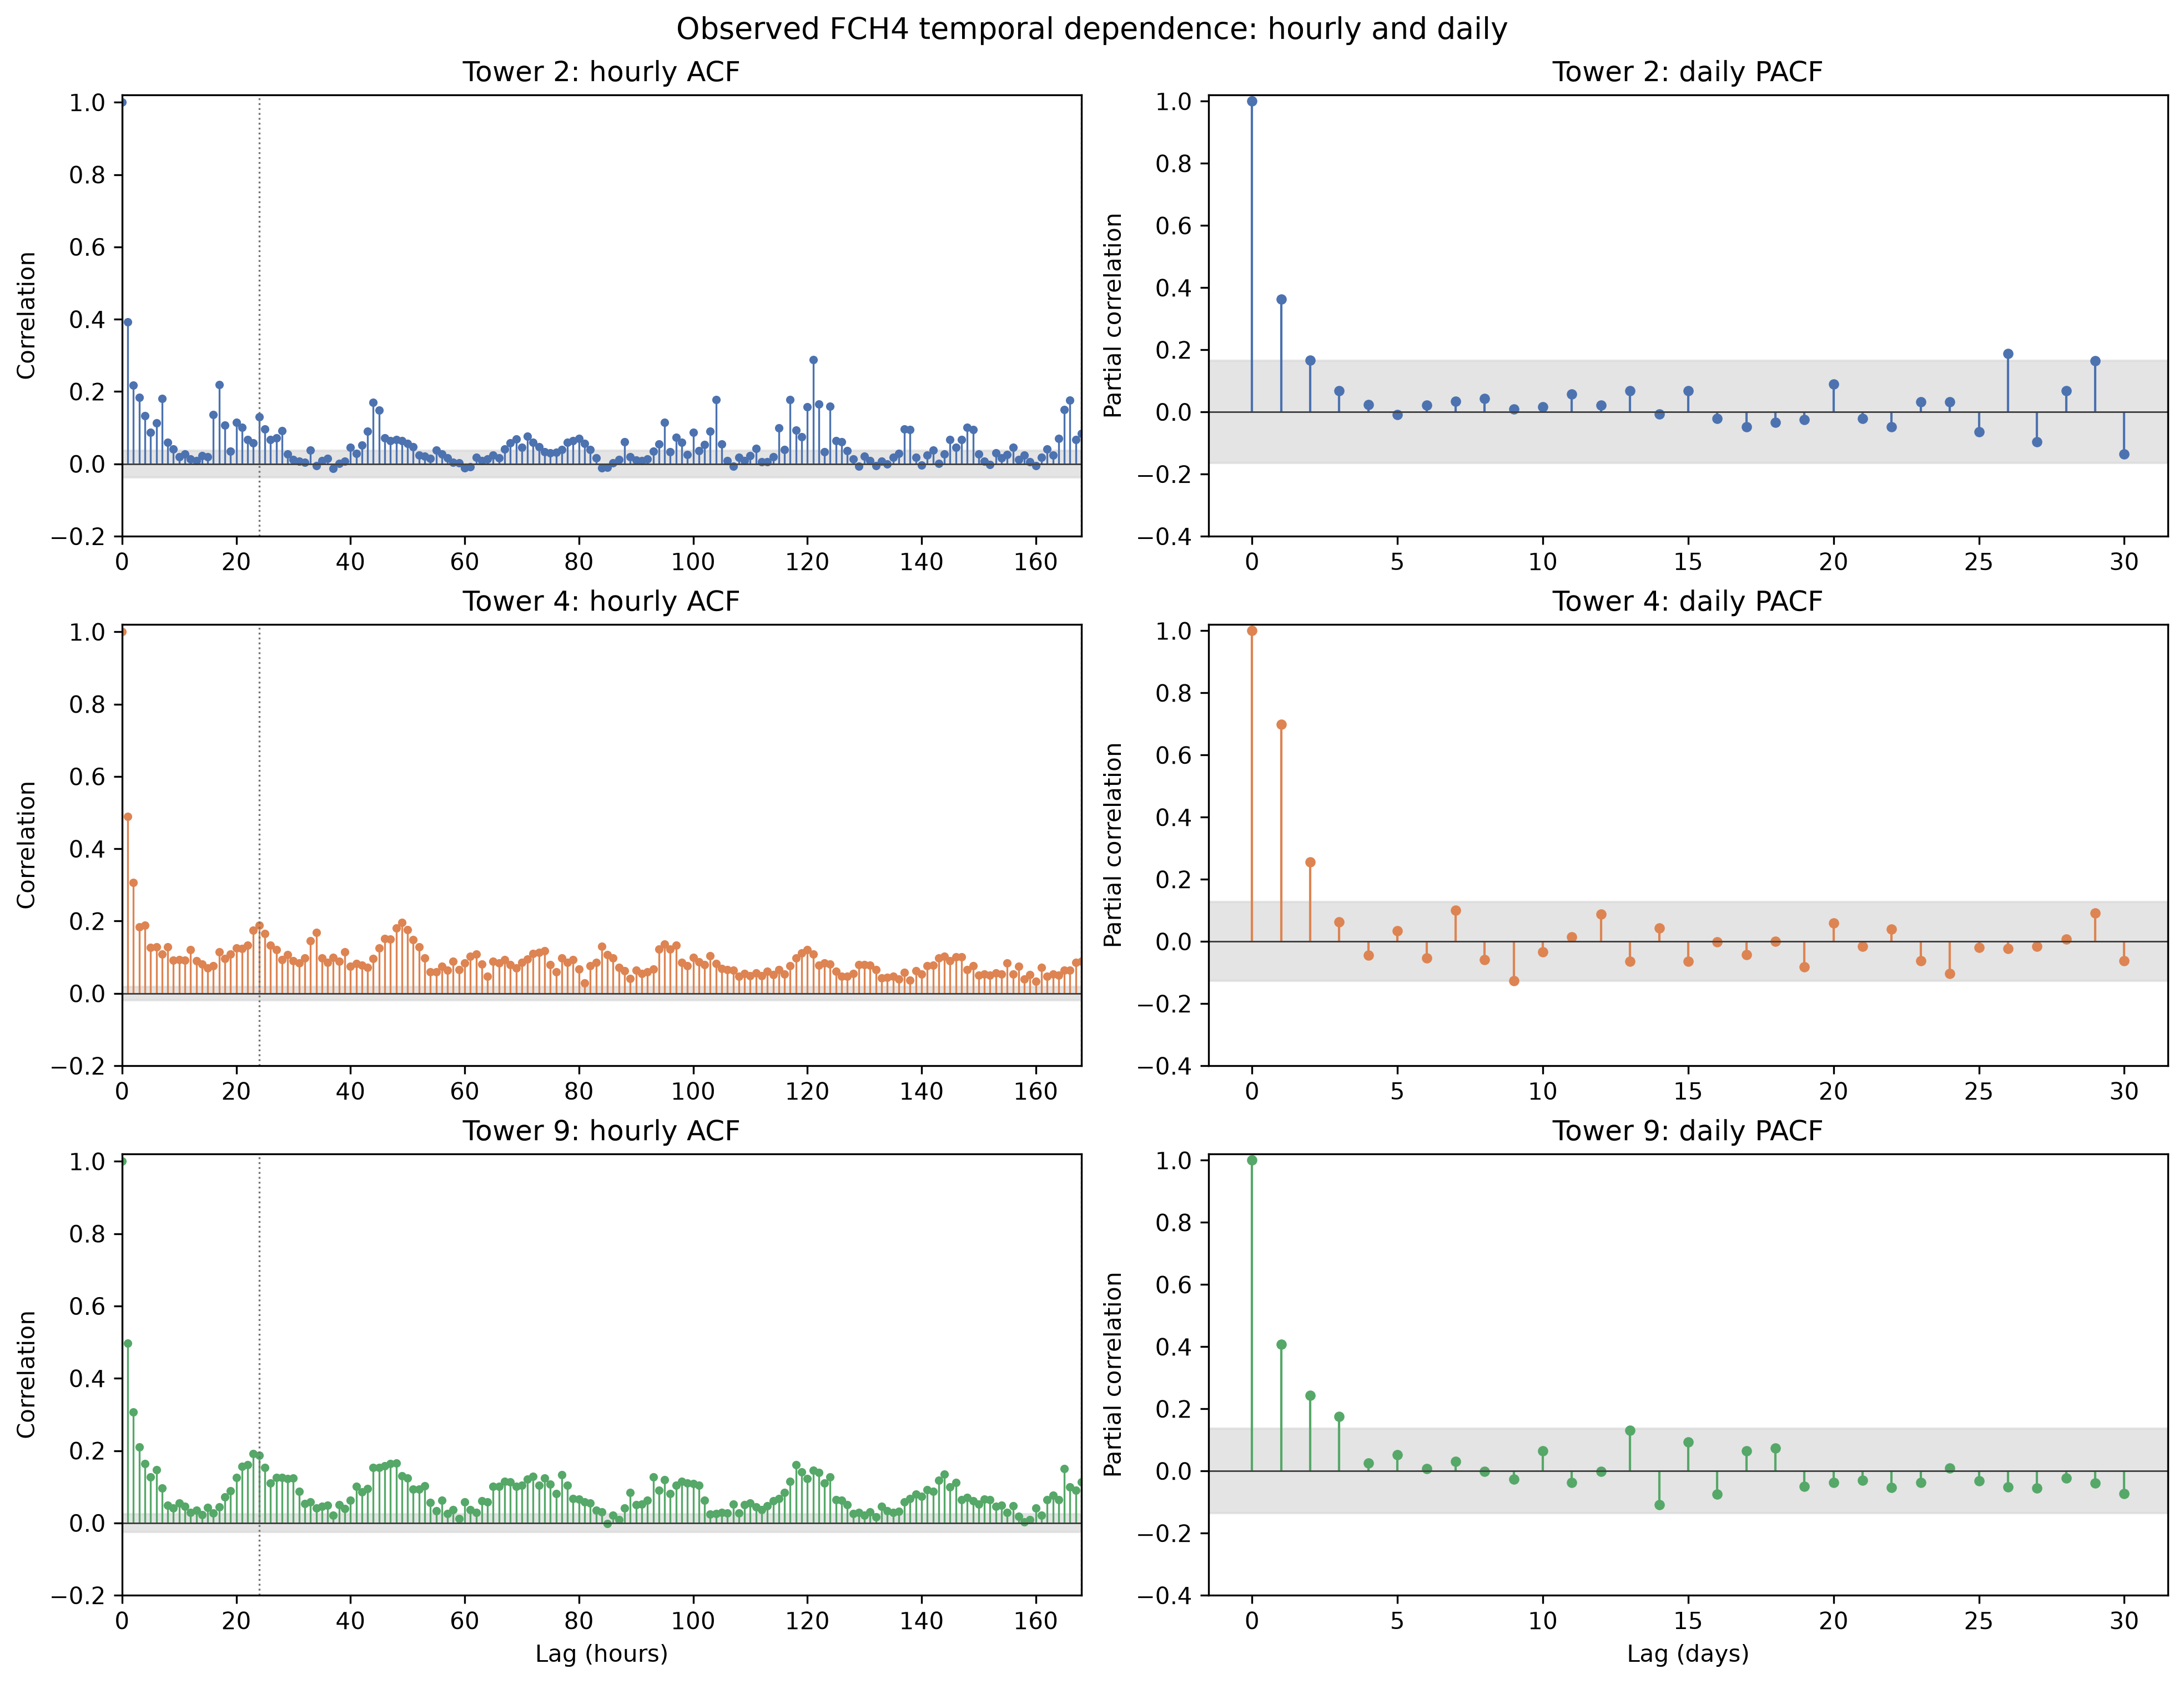
\includegraphics[width=\textwidth]{Figures/ch3_acf_pacf_observed.png}
\caption{
    Temporal dependence of QC-valid observed
  FCH\textsubscript{4}. Left: hourly ACF calculated from available
  observation pairs at each lag, with 24 hours marked by the dotted line.
  Right: daily PACF calculated over the longest sufficiently complete
  segment at each tower; shaded regions show approximate 95\% confidence
  bounds.
}
\label{fig:appendix_ch3_acf_pacf}
\end{figure}

\begin{figure}[htbp]
\centering
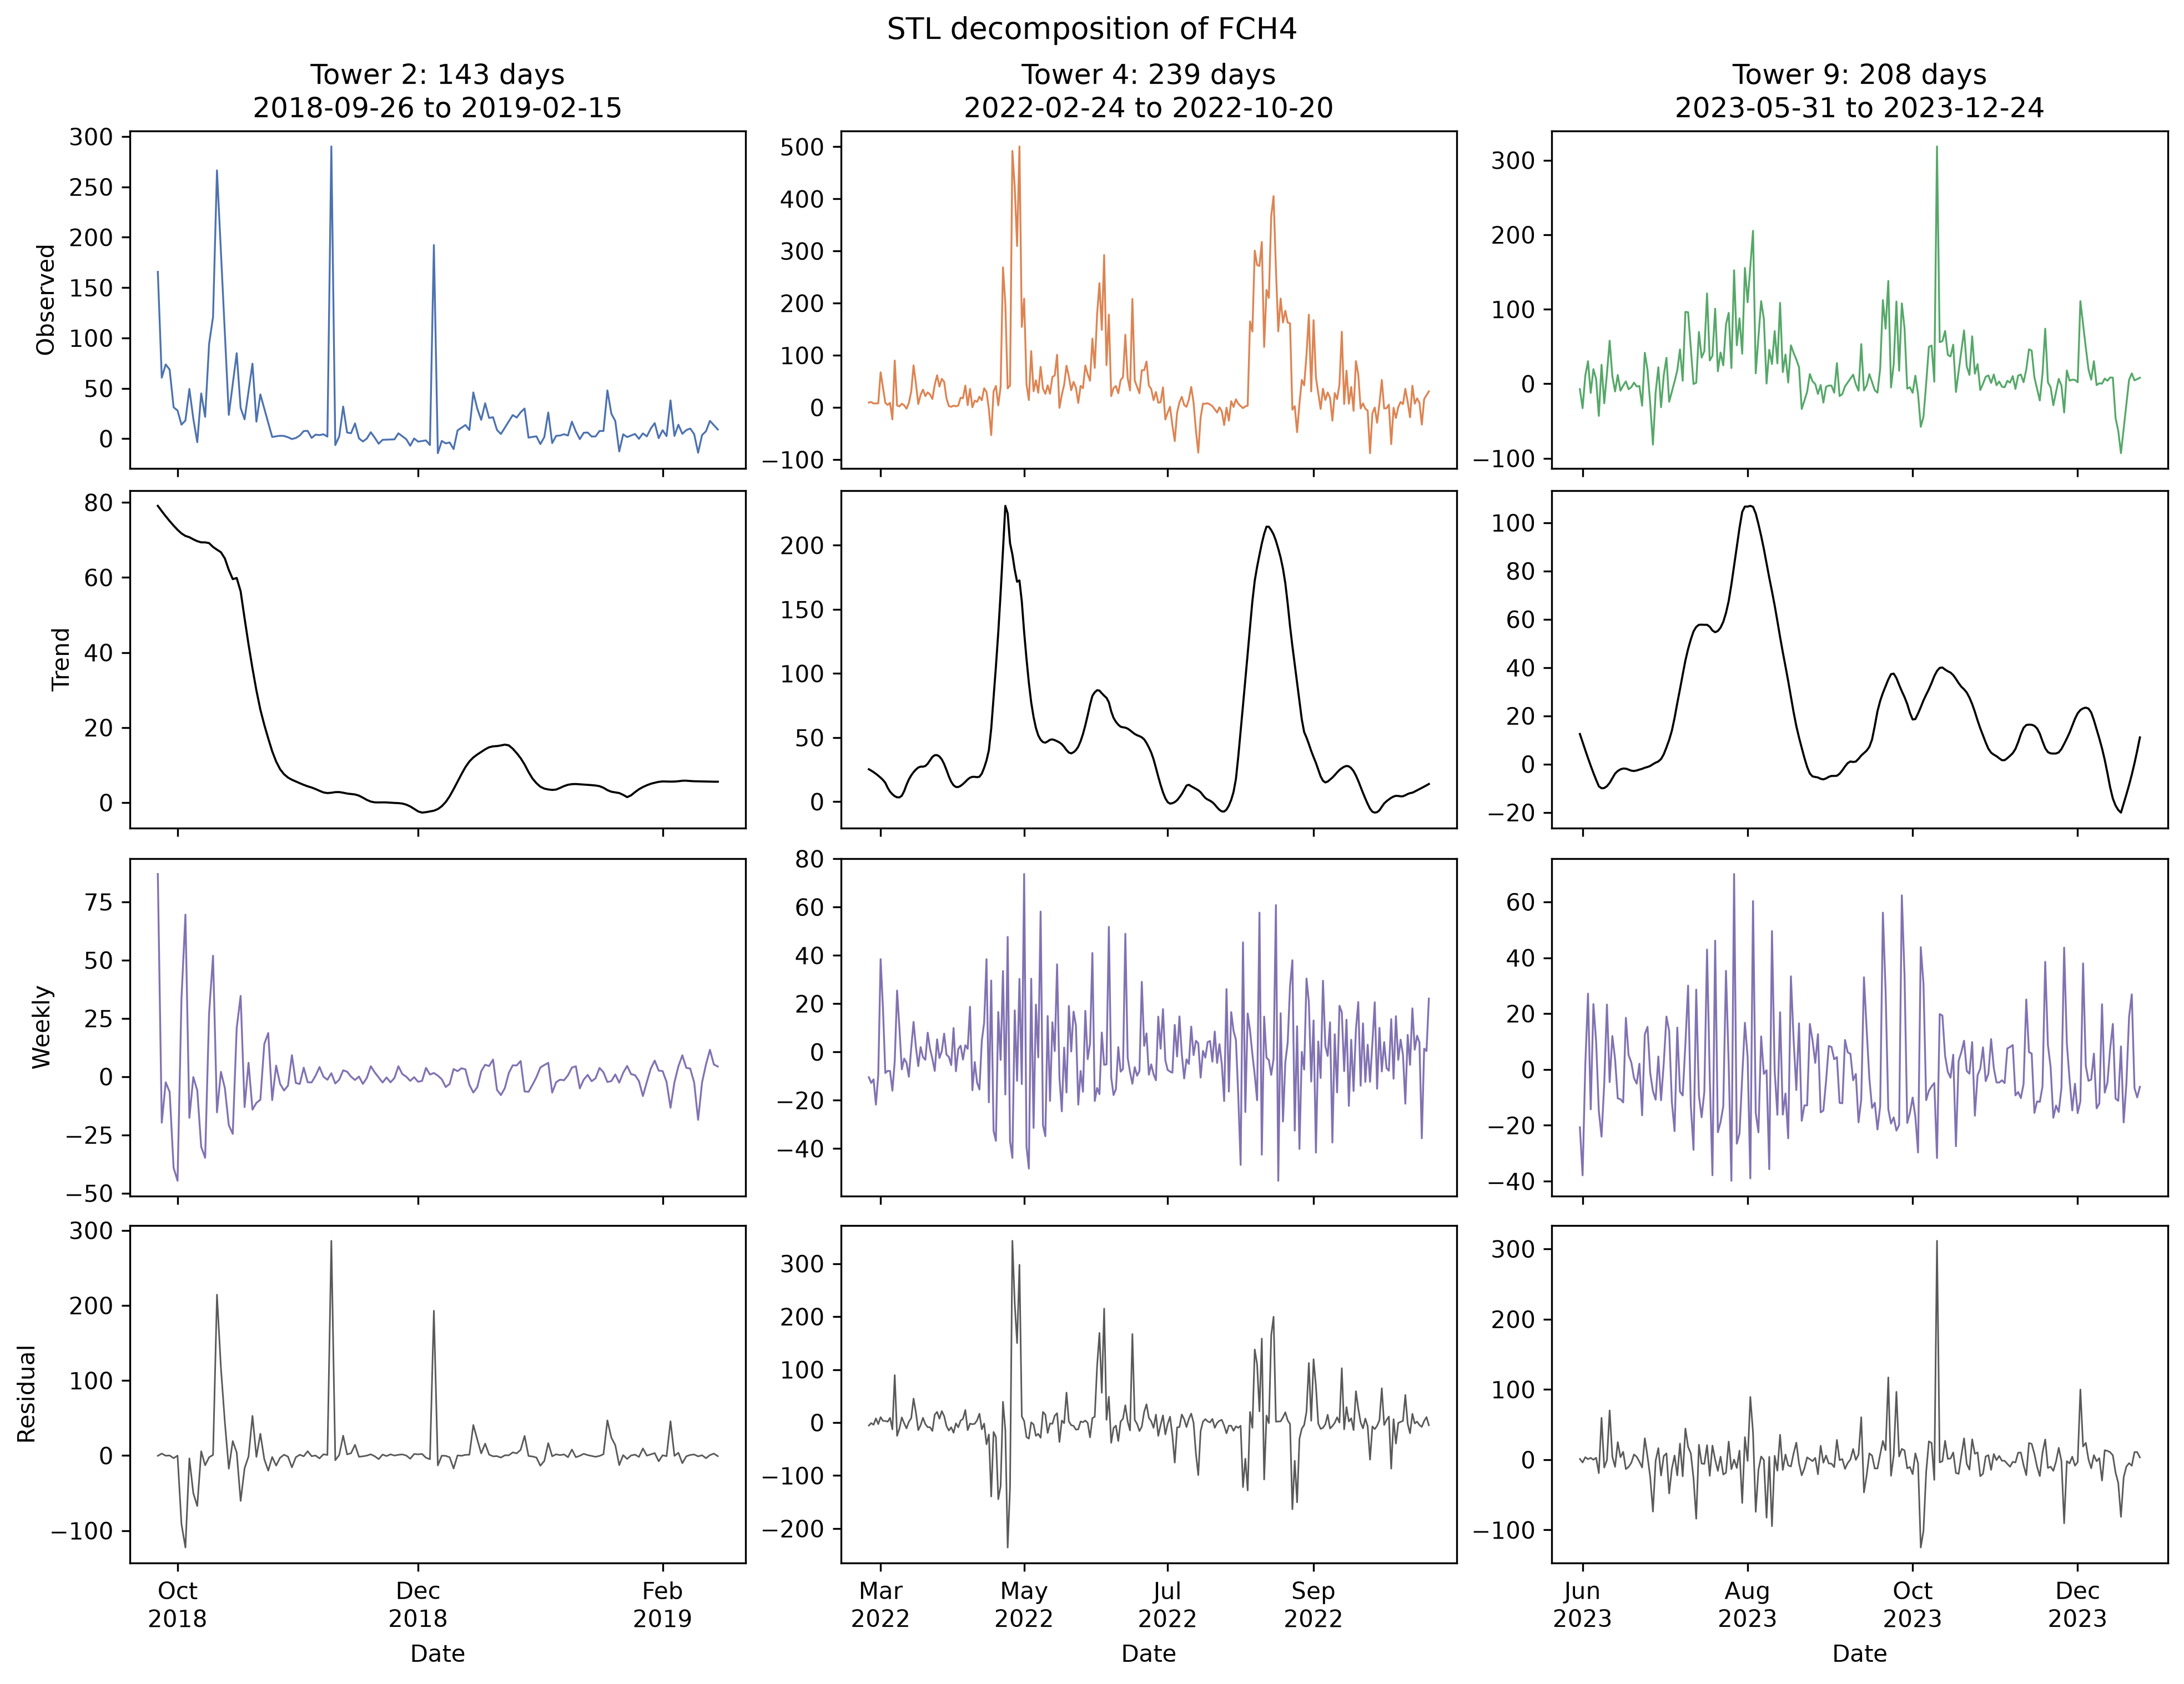
\includegraphics[width=\textwidth]{Figures/ch3_stl_decomposition_observed.png}
\caption{
    Weekly STL decomposition of the longest sufficiently complete
  daily FCH\textsubscript{4} segment at each tower. Rows show the observed
  series, trend, weekly component and residual. 
}
\label{fig:appendix_ch3_stl}
\end{figure}

\FloatBarrier


\chapter{Models}
\label{app:model-algorithms}

This appendix supplements the operating-principle summary in
Table~\ref{tab:model_roster} with model-specific pseudocode. The common
synthetic-gap and fixed-origin forecasting protocols remain defined in
Chapter~\ref{ChapModels}; they are not repeated here. Likewise,
Algorithm~\ref{alg:auxiliary-driver-gapfill} already documents auxiliary
environmental-driver reconstruction. The algorithms below therefore focus on
how each benchmark model learns or produces predictions. ``GF'' denotes
gap-filling and ``FC'' denotes forecasting.

\section{Multivariate Imputation}

MICE and HyperImpute treat FCH\textsubscript{4} as an incomplete column in a
joint feature--target matrix. MICE uses a fixed Bayesian-ridge conditional
model \cite{vanbuuren2011mice}, whereas HyperImpute selects a conditional
learner separately for each variable through internal validation
\cite{jarrett2022hyperimpute}.

\begin{algorithm}[H]
\caption{MICE reconstruction with Bayesian-ridge conditional models}
\label{alg:app-mice}
\small
\begin{algorithmic}[1]
\Require Pooled incomplete matrix $Z=[y,X,\text{tower indicators}]$;
held-out target positions $H$
\Ensure Reconstructed target $\hat y_H$
\State Set $Z_{H,y}$ to missing before constructing the imputer input
\State Initialise each incomplete column from its observed marginal values
\For{chained iteration $q\gets1$ to $K$}
    \For{each incomplete column $j$}
        \State Define observed rows $O_j$ and missing rows $M_j$
        \State Fit Bayesian ridge $f_j^{(q)}:Z_{O_j,-j}\mapsto Z_{O_j,j}$
        \State Update $Z_{M_j,j}\gets f_j^{(q)}(Z_{M_j,-j})$
    \EndFor
    \If{the iterative-imputer convergence rule is satisfied}
        \State Break
    \EndIf
\EndFor
\State Extract $\hat y_H\gets Z_{H,y}$ using the held-out rows' absolute positions
\State \Return $\hat y_H$
\end{algorithmic}
\end{algorithm}

\begin{algorithm}[H]
\caption{HyperImpute reconstruction with variable-specific AutoML models}
\label{alg:app-hyperimpute}
\small
\begin{algorithmic}[1]
\Require Pooled incomplete matrix $Z=[y,X,\text{tower indicators}]$;
held-out positions $H$; candidate learner library $\mathcal L$
\Ensure Reconstructed target $\hat y_H$
\State Set $Z_{H,y}$ to missing and initialise incomplete columns
\For{each chained-imputation round}
    \For{each incomplete column $j$}
        \State Determine whether $Z_j$ requires regression or classification
        \For{each compatible learner $f\in\mathcal L$}
            \State Estimate internal validation loss $L_j(f)$ on observed rows $O_j$
        \EndFor
        \State Select $f_j^*\gets\arg\min_{f\in\mathcal L}L_j(f)$
        \State Refit $f_j^*$ on $O_j$ and update
        $Z_{M_j,j}\gets f_j^*(Z_{M_j,-j})$
    \EndFor
    \If{the imputation sequence converges or reaches its iteration limit}
        \State Break
    \EndIf
\EndFor
\State \Return the completed target values $\hat y_H$
\end{algorithmic}
\end{algorithm}

\section{Tree-Based Models}

Random Forest, XGBoost and LightGBM were used in both tasks. For gap-filling,
the query rows are the deliberately masked hours. For forecasting, each model
is fitted at a forecast origin and its predicted FCH\textsubscript{4} value is
appended to the available target history before constructing the next day's
autoregressive features. Preprocessing is always estimated from permitted
training rows. The algorithms follow Breiman \cite{breiman2001randomforests},
Chen and Guestrin \cite{chen2016xgboost}, and Ke et al.\ \cite{ke2017lightgbm}.
The unweighted voting-regression ensemble then averages the three aligned
forecast chains following the forecast-combination principle of Bates and
Granger \cite{bates1969combination}.

\begin{algorithm}[H]
\caption{Random Forest reconstruction or recursive forecasting}
\label{alg:app-rf}
\small
\begin{algorithmic}[1]
\Require Training rows $(X_O,y_O)$; query rows $X_Q$; number of trees $B$;
minimum leaf size $m$; task $\tau\in\{\mathrm{GF},\mathrm{FC}\}$
\Ensure Predictions $\hat y_Q$
\State Fit mean imputation on $X_O$ and apply it to $X_O$ and $X_Q$
\State Use $(B,m)=(500,5)$ for GF and $(500,10)$ for FC
\For{$b\gets1$ to $B$}
    \State Draw a bootstrap sample of $(X_O,y_O)$
    \State Grow $T_b$ using squared-error reduction and random candidate features
    \State Stop a branch when further splitting violates the minimum leaf size
\EndFor
\State Define $f(x)\gets B^{-1}\sum_{b=1}^{B}T_b(x)$
\If{$\tau=\mathrm{GF}$}
    \State Predict the masked hourly rows directly: $\hat y_Q\gets f(X_Q)$
\Else
    \For{forecast day $h\gets1$ to $365$}
        \State Build day-$h$ features from known covariates and available target history
        \State Predict $\hat y_h\gets f(x_h)$ and append $\hat y_h$ to that history
    \EndFor
\EndIf
\State \Return $\hat y_Q$
\end{algorithmic}
\end{algorithm}

\begin{algorithm}[H]
\caption{XGBoost reconstruction or recursive forecasting}
\label{alg:app-xgboost}
\small
\begin{algorithmic}[1]
\Require Training rows $(X_O,y_O)$; query rows $X_Q$; boosting rounds $B$;
learning rate $\eta$
\Ensure Predictions $\hat y_Q$
\State Fit training-only predictor imputation and initialise $F_0(x)$ with a constant
\For{$b\gets1$ to $B$}
    \For{each $i\in O$}
        \State Compute $g_i=\partial_F\ell(y_i,F_{b-1}(x_i))$ and
        $h_i=\partial_F^2\ell(y_i,F_{b-1}(x_i))$
    \EndFor
    \State Grow $T_b$ by maximising regularised split gain from sums of $g_i$ and $h_i$
    \State Assign each leaf its regularised optimum weight
    \State Update $F_b(x)\gets F_{b-1}(x)+\eta T_b(x)$
\EndFor
\State Use 500 rounds and minimum child weight 5 for GF
\State Use 400 rounds, depth 2, $\eta=0.02$ and minimum child weight 10 for FC
\State Predict GF rows directly or generate the FC chain by appending each prediction
\State \Return $F_B(X_Q)$ or the resulting recursive chain
\end{algorithmic}
\end{algorithm}

\begin{algorithm}[H]
\caption{LightGBM reconstruction or recursive forecasting}
\label{alg:app-lightgbm}
\small
\begin{algorithmic}[1]
\Require Training rows $(X_O,y_O)$; query rows $X_Q$; boosting rounds $B$;
learning rate $\eta$
\Ensure Predictions $\hat y_Q$
\State Fit training-only predictor imputation and bin continuous predictors
\State Initialise $F_0(x)$ with a constant
\For{$b\gets1$ to $B$}
    \State Calculate loss gradients from $y_O$ and $F_{b-1}(X_O)$
    \State Accumulate gradient statistics by feature-histogram bin
    \While{a permissible positive-gain split exists}
        \State Split the leaf giving the greatest loss reduction
    \EndWhile
    \State Update $F_b(x)\gets F_{b-1}(x)+\eta T_b(x)$
\EndFor
\State Use 500 rounds and minimum child size 5 for GF
\State Use 400 rounds, 7 leaves, $\eta=0.02$ and minimum child size 10 for FC
\State Predict GF rows directly or recursively update the FC target history
\State \Return $F_B(X_Q)$ or the resulting recursive chain
\end{algorithmic}
\end{algorithm}

\begin{algorithm}[H]
\caption{Unweighted voting-regression forecast ensemble}
\label{alg:app-unweighted-voting-regression}
\small
\begin{algorithmic}[1]
\Require Aligned Random Forest, XGBoost and LightGBM forecast chains
\Ensure Equal-weight ensemble forecast $\hat y^{ens}$
\For{each tower, origin and forecast day $t$}
    \State Verify that all component predictions refer to the same target row
    \State $\hat y_t^{ens}\gets
    (\hat y_t^{RF}+\hat y_t^{XGB}+\hat y_t^{LGBM})/3$
\EndFor
\State Evaluate the ensemble only at QC-valid observed target rows
\State \Return $\hat y^{ens}$
\end{algorithmic}
\end{algorithm}

\section{Neural Models}

The ANN is retained as a published-baseline replication
\cite{rumelhart1986backprop}. SAITS and the bidirectional LSTM use observations
on both sides of historical gaps, whereas the forecasting LSTM, TFT and DLinear
operate causally beyond each forecast origin
\cite{du2023saits,hochreiter1997lstm,schuster1997bidirectional,lim2021tft,zeng2023}.

\begin{algorithm}[H]
\caption{Feed-forward ANN gap reconstruction}
\label{alg:app-ann}
\small
\begin{algorithmic}[1]
\Require Standardised observed pairs $(X_O,y_O)$; masked queries $X_H$;
network layers $1{:}L$
\Ensure Reconstructed target $\hat y_H$
\State Initialise weights $W^{(\ell)}$ and biases $b^{(\ell)}$
\For{each training epoch}
    \State Set $a^{(0)}\gets X_O$
    \For{$\ell\gets1$ to $L-1$}
        \State $a^{(\ell)}\gets\phi(W^{(\ell)}a^{(\ell-1)}+b^{(\ell)})$
    \EndFor
    \State $\hat y\gets W^{(L)}a^{(L-1)}+b^{(L)}$
    \State Back-propagate prediction loss and update all trainable parameters
\EndFor
\State Apply the fitted network to $X_H$ and reverse target scaling
\State \Return $\hat y_H$
\end{algorithmic}
\end{algorithm}

\begin{algorithm}[H]
\caption{SAITS diagonally masked attention reconstruction}
\label{alg:app-saits}
\small
\begin{algorithmic}[1]
\Require Per-tower sequence $Z=[X,y]$ with $y_H$ masked; 336-hour windows;
24-hour stride
\Ensure Reconstructed target $\hat y_H$
\State Remove the eight explicit soil-lag channels and standardise the masked sequence
\State Create overlapping windows and a chronological training--validation split
\State Initialise 3 layers, $d_{model}=256$, 4 heads, $d_k=d_v=64$,
$d_{ff}=512$, dropout 0.1
\For{epoch $e\gets1$ to $100$}
    \State Compute diagonally masked attention
    $A=\operatorname{softmax}(QK^\top/\sqrt{d_k}+D)V$, where $D_{tt}=-\infty$
    \State Obtain reconstructions $\widetilde Z^{(1)}$ and $\widetilde Z^{(2)}$
    \State Combine them as
    $\widetilde Z=\beta\odot\widetilde Z^{(1)}+(1-\beta)\odot\widetilde Z^{(2)}$
    \State Minimise spike-weighted absolute reconstruction error in batches of 32
    \State Retain the best validation state; stop after 10 non-improving epochs
\EndFor
\State Average overlapping estimates, reverse scaling and \Return values at $H$
\end{algorithmic}
\end{algorithm}

\begin{algorithm}[H]
\caption{Bidirectional LSTM gap reconstruction}
\label{alg:app-bilstm}
\small
\begin{algorithmic}[1]
\Require Standardised 336-hour windows $[X,y]$; observation mask $m$;
held-out set $H$
\Ensure Reconstructed target $\hat y_H$
\State Replace missing target inputs by zero and append mask $m_t$ as an input channel
\State Initialise a two-layer Bi-LSTM with 128 hidden units per direction and dropout 0.1
\For{epoch $e\gets1$ to $50$}
    \State Randomly mask 20\% of observed targets to form reconstruction mask $\widetilde m$
    \State $\overrightarrow h_t\gets\operatorname{LSTM}(u_t,\overrightarrow h_{t-1})$
    \State $\overleftarrow h_t\gets\operatorname{LSTM}(u_t,\overleftarrow h_{t+1})$
    \State $\hat y_t\gets W[\overrightarrow h_t;\overleftarrow h_t]+b$
    \State Minimise
    $\sum_t\widetilde m_t(1+|y_t|)|y_t-\hat y_t|/\sum_t\widetilde m_t$
    using Adam and learning rate $10^{-3}$
    \State Retain the best validation state; stop after 8 non-improving epochs
\EndFor
\State Average overlapping estimates, reverse scaling and \Return values at $H$
\end{algorithmic}
\end{algorithm}

\begin{algorithm}[H]
\caption{Causal LSTM forecasting}
\label{alg:app-lstm-forecast}
\small
\begin{algorithmic}[1]
\Require Pre-origin daily target and drivers; 28-day lookback; hidden size 64
\Ensure Continuous 365-day forecast
\State Form training windows ending no later than the forecast origin
\State Standardise using pre-origin training statistics
\For{each training window and time $t$}
    \State Compute input, forget and output gates $i_t,f_t,o_t$
    \State $\widetilde c_t\gets\tanh(W_cu_t+U_ch_{t-1}+b_c)$
    \State $c_t\gets f_t\odot c_{t-1}+i_t\odot\widetilde c_t$
    \State $h_t\gets o_t\odot\tanh(c_t)$ and map $h_t$ to the next target
    \State Update parameters by back-propagation through time
\EndFor
\For{forecast day $h\gets1$ to $365$}
    \State Predict from the latest 28 permitted days and known day-$h$ drivers
    \State Append the prediction, rather than the later observation, to the history
\EndFor
\State Reverse target scaling and \Return the forecast chain
\end{algorithmic}
\end{algorithm}

\begin{algorithm}[H]
\caption{Temporal Fusion Transformer forecasting}
\label{alg:app-tft}
\small
\begin{algorithmic}[1]
\Require Pre-origin daily sequences; known-future covariates; 28-day lookback;
$d_{model}=32$; 4 heads; dropout 0.1
\Ensure Continuous 365-day forecast and optional quantiles
\State Encode static, observed-history and known-future variables separately
\State Apply variable-selection networks to obtain time-varying feature weights
\State Pass selected inputs through gated residual networks and an LSTM encoder--decoder
\State Apply causal temporal attention over permitted positions
\State Produce point or quantile outputs through the gated output head
\For{forecast day $h\gets1$ to $365$}
    \State Supply the latest 28-day context and covariates known for day $h$
    \State Retain the next prediction and append it to the target history
\EndFor
\State \Return the continuous chain and any requested quantiles
\end{algorithmic}
\end{algorithm}

\begin{algorithm}[H]
\caption{DLinear decomposition forecasting}
\label{alg:app-dlinear}
\small
\begin{algorithmic}[1]
\Require Pre-origin daily sequence $z_{t-27:t}$; moving-average kernel 25
\Ensure Continuous 365-day forecast
\State Estimate trend $\tau\gets\operatorname{MovingAverage}_{25}(z)$
\State Calculate residual component $s\gets z-\tau$
\State Learn linear projections $W_\tau,b_\tau$ and $W_s,b_s$ from training windows
\State Define $\hat z\gets(W_\tau\tau+b_\tau)+(W_ss+b_s)$
\For{forecast day $h\gets1$ to $365$}
    \State Predict from the latest 28-day sequence
    \State Append the prediction and advance the input window by one day
\EndFor
\State Reverse target scaling and \Return the continuous chain
\end{algorithmic}
\end{algorithm}

\section{Statistical and Kernel Models}

Support-vector regression is retained as a literature-aligned gap-filling
replication \cite{drucker1997svr}. SARIMAX provides the forecasting benchmark
with an explicit stochastic time-series structure \cite{box2015timeseries}.

\begin{algorithm}[H]
\caption{$\epsilon$-support-vector regression gap reconstruction}
\label{alg:app-svr}
\small
\begin{algorithmic}[1]
\Require Standardised training pairs $(X_O,y_O)$; queries $X_H$; kernel $K$;
penalty $C$; tube width $\epsilon$
\Ensure Reconstructed target $\hat y_H$
\State Solve
$\min_{w,b,\xi,\xi^*}\frac12\lVert w\rVert^2+C\sum_i(\xi_i+\xi_i^*)$
subject to $|y_i-(w^\top\phi(x_i)+b)|\le\epsilon+\xi_i$
\State Retain rows with non-zero dual coefficients as support vectors
\State Define
$\hat y(x)\gets\sum_{i\in O}(\alpha_i-\alpha_i^*)K(x_i,x)+b$
\State Reverse target scaling and \Return $\hat y(X_H)$
\end{algorithmic}
\end{algorithm}

\begin{algorithm}[H]
\caption{AIC-selected SARIMAX forecasting}
\label{alg:app-sarimax}
\small
\begin{algorithmic}[1]
\Require Per-tower pre-origin target $y_t$; exogenous vector $x_t$;
$p\in\{1,2\}$, $d=1$, $q\in\{0,1\}$
\Ensure Continuous 365-day forecast
\For{each candidate order $(p,1,q)$}
    \State Fit
    $\Phi_p(B)(1-B)y_t=c+\beta^\top x_t+\Theta_q(B)\varepsilon_t$
    by maximum likelihood on pre-origin observations
    \State Calculate $\mathrm{AIC}=2k-2\log\widehat L$
\EndFor
\State Select the converged candidate with minimum AIC
\State Forecast 365 steps using its dynamic state update and known future $x_t$
\State Propagate the state without inserting later observed FCH\textsubscript{4}
\State \Return predictive means and state-space intervals
\end{algorithmic}
\end{algorithm}

\section{Pretrained Tabular Models}

\subsection{Pretraining and in-context adaptation}

TabPFN and TabICLv2 are prior-data fitted networks (PFNs).  Their model
parameters are learned once, before application to this study, across a large
distribution of synthetic tabular prediction tasks.  For a synthetic task
$\mathcal T\sim p_{\mathrm{synth}}$, rows are divided into a labelled context
$\mathcal D_C=(X_C,y_C)$ and an unlabelled query $X_Q$ with held-out target
$y_Q$.  Pretraining minimises the query negative log-likelihood,
\begin{equation}
\theta^*=\arg\min_\theta
\mathbb E_{\mathcal T\sim p_{\mathrm{synth}}}
\left[-\sum_{j\in Q}\log q_\theta
\left(y_j\mid x_j,\mathcal D_C\right)\right],
\label{eq:app-pfn-pretraining}
\end{equation}
so that one forward pass subsequently approximates the posterior predictive
rule induced by the synthetic task prior
\cite{hollmann2023tabpfn,hollmann2025tabpfn,qu2025tabicl,qu2026tabiclv2}.
This is amortised inference: the expensive learning occurs across synthetic
tasks during offline pretraining, rather than through gradient optimisation on
each new dataset.

TabPFN v2 retains a representation for every table cell.  Numerical values are
combined with feature-specific random embeddings, grouped in pairs, and passed
through 12 Transformer blocks (192-dimensional embeddings and six attention
heads).  Each block alternates attention across features within a row and
across samples within a feature.  Context targets are embedded while query
targets remain masked, allowing queries to attend to labelled examples without
target leakage.  For regression, the output head assigns probability to target
intervals through a full-support bar distribution and is trained by negative
log-likelihood; means, medians or quantiles are then derived from this
distribution \cite{hollmann2025tabpfn}.

Its synthetic prior samples table properties and structural causal models:
random directed acyclic graphs are populated with nonlinear mechanisms,
transformations, feature types, missingness and noise.  Approximately 100
million such tasks expose the model to varied tabular relationships.  This
study used the released generic \texttt{tabpfn-v2-\allowbreak regressor.ckpt}, not a
time-series-fine-tuned checkpoint.

TabICLv2 instead compresses features before dataset-level inference.  Repeated
circular feature groups are given target-aware embeddings for labelled rows; a
column Transformer processes each feature across samples, and a row Transformer
combines the features into a 512-dimensional representation.  A 12-layer
dataset Transformer then relates labelled and query rows.  Its query-aware
scalable softmax (QASSMax) counters attention dilution as the context grows,
reducing the principal scaling from approximately
$O(n^2m+nm^2)$ for cell-level TabPFN to $O(n^2+nm^2)$
\cite{qu2025tabicl,qu2026tabiclv2}.

TabICLv2 is pretrained on approximately 35 million filtered synthetic tasks
generated by random graphs containing neural, tree, Gaussian-process, linear,
quadratic, product and discretisation mechanisms.  Its three-stage curriculum
increases contexts from 1,024 to at most 60,000 rows and 100 features.  The
regression model uses Muon optimisation and pinball loss over 999 conditional
quantiles.  Thus, unlike squared-error regressors, neither TabPFN nor TabICLv2
directly optimises the downstream $R^2$, RMSE, MAE or MASE metrics.

Neither checkpoint was pretrained on North Wyke Farm Platform data, methane
fluxes or the held-out forecast years.  Here, \texttt{fit()} only preprocesses
and registers the chronologically permitted labelled context; it does not
update $\theta^*$.  Temporal information therefore enters through context
selection and the engineered calendar, environmental and management features.
The direct forecasting configuration used eight internal estimators (TabPFN
seed 137; TabICLv2 seed 42) without checkpoint fine-tuning.  Forecast
combinations follow Bates and Granger's variance-reduction principle
\cite{bates1969combination}.

\begin{algorithm}[H]
\caption{Published offline pretraining scheme for TabPFN and TabICLv2}
\label{alg:app-pfn-pretraining}
\small
\begin{algorithmic}[1]
\Require Model family $M\in\{\mathrm{TabPFN},\mathrm{TabICLv2}\}$;
synthetic task prior $p_{\mathrm{synth}}^M$; model $q_\theta$
\Ensure Released pretrained checkpoint $\theta^*$
\For{each offline pretraining step}
    \State Sample table dimensions, feature types and task difficulty
    \If{$M=\mathrm{TabPFN}$}
        \State Sample an SCM directed acyclic graph, node mechanisms and noise
    \Else
        \State Sample a random graph with mixed neural, tree, GP and algebraic mechanisms
    \EndIf
    \State Generate a synthetic table $\mathcal T=(X,y)$ and apply model-specific filtering
    \State Split rows into labelled context $\mathcal D_C$ and query $(X_Q,y_Q)$
    \State Predict $q_\theta(y_Q\mid X_Q,\mathcal D_C)$ in one forward pass
    \If{$M=\mathrm{TabPFN}$}
        \State Compute the discretised regression negative log-likelihood and update with Adam
    \Else
        \State Sum pinball losses over 999 quantiles and update with Muon
        \State Advance the three-stage table-size curriculum
    \EndIf
\EndFor
\State Freeze the final parameters; no study data enter this procedure
\State \Return $\theta^*$ for subsequent in-context inference
\end{algorithmic}
\end{algorithm}

\begin{algorithm}[H]
\caption{TabPFN inference for gap filling or direct daily forecasting}
\label{alg:app-tabpfn}
\small
\begin{algorithmic}[1]
\Require Labelled context $\mathcal D_C=\{(x_i,y_i)\}$; query features $X_Q$;
pretrained parameters $\theta$; task $\tau$
\Ensure Predictive distribution and point predictions
\If{$\tau=\mathrm{GF}$}
    \State Construct an hourly tabular task after masking $y_H$ and exclude $H$ from context
\Else
    \State Use pre-origin daily rows and the 52-driver plus 5 tower/time-indicator frame
    \State Optionally restrict context to the most recent 1,095 or 1,460 days
\EndIf
\State Fit training-only missing-value preprocessing and configured target scaling
\State Jointly encode labelled context and unlabelled query rows with the pretrained model
\State Infer $p_\theta(y_Q\mid\mathcal D_C,X_Q)$ without gradient-based task training
\State Extract the configured point statistic (median for direct forecasts) and quantiles
\State Reverse target scaling and \Return predictions
\end{algorithmic}
\end{algorithm}

\begin{algorithm}[H]
\caption{TabICLv2 inference for gap filling or direct daily forecasting}
\label{alg:app-tabicl}
\small
\begin{algorithmic}[1]
\Require Labelled context $\mathcal D_C$; query features $X_Q$;
pretrained parameters $\theta$; task $\tau$
\Ensure Point predictions and optional quantiles
\If{$\tau=\mathrm{GF}$}
    \State Train separately by tower on the expanded 30-predictor frame
    \State Exclude $H$ and sample at most 10,000 observed rows using seed 42
    \State Mean-impute predictors using the sampled context
\Else
    \State Use pre-origin daily context and the applicable forecasting frame
    \State Optionally retain all history, 1,095 days or 1,460 days
    \State Apply tower-wise target scaling for the configured 1,460-day variant
\EndIf
\State Register the labelled context through the model fit interface
\State Keep the pretrained checkpoint fixed; \texttt{fit()} performs no gradient update
\State Infer $p_\theta(y_Q\mid\mathcal D_C,X_Q)$ jointly from context and queries
\State Extract the median point prediction and optional 0.05, 0.50 and 0.95 quantiles
\State Reverse target scaling and \Return predictions
\end{algorithmic}
\end{algorithm}

\begin{algorithm}[H]
\caption{Probability-gated spike correction for a foundation-model forecast}
\label{alg:app-spike-correction}
\small
\begin{algorithmic}[1]
\Require Base regressor $f_b$; spike classifier $c$; spike regressor $f_s$;
normal regressor $f_n$; pre-origin tower-specific 95th percentile $q_{0.95}$
\Ensure Corrected forecast $\hat y^{corr}$
\State Label context row $i$ as a spike if $y_i>q_{0.95}$
\State Fit or condition $c$, $f_s$, $f_n$ and $f_b$ using permitted context only
\For{each query day $t$}
    \State $p_t^{spike}\gets c(x_t)$
    \State $e_t\gets[f_s(x_t)-f_n(x_t)]_+$
    \State $\hat y_t^{corr}\gets f_b(x_t)+0.25\,p_t^{spike}e_t$
\EndFor
\State \Return $\hat y^{corr}$
\end{algorithmic}
\end{algorithm}

\begin{algorithm}[H]
\caption{Best-performing TabICL forecasting model}
\label{alg:app-best-tabicl-forecast}
\small
\begin{algorithmic}[1]
\Require TabICLv2 forecaster $F$; pre-origin daily data; 365-day queries
\Ensure Final blended forecast $\hat y^{\mathrm{best}}$
\State $\hat y^{(1)}\gets$ all-history forecast from $F$ with
Algorithm~\ref{alg:app-spike-correction}
\State $\hat y^{(2)}\gets$ forecast from $F$ using the latest 1,095 context days
\State $\hat y^{(3)}\gets$ forecast from $F$ using the latest 1,460 context days and
tower-wise target scaling
\For{each forecast day $t$}
    \State $\hat y_t^{\mathrm{best}}\gets
    (\hat y_t^{(1)}+\hat y_t^{(2)}+\hat y_t^{(3)})/3$
\EndFor
\State Retain the three component chains and evaluate the blend on identical observed rows
\State \Return $\hat y^{\mathrm{best}}$
\end{algorithmic}
\end{algorithm}

\FloatBarrier


\chapter{Gap-Filling}
\label{app:gap-filling}

Table~\ref{tab:gf_published_replication} records the source-specific methane
gap-filling adaptations removed from the main chapter. Differences in
ecosystem, predictors, measurement period and validation design mean that the
reported source values provide context rather than controlled performance
comparisons \cite{irvin2021,kim2020,zhu2023a}.

\begin{table}[htbp]
\centering
\footnotesize
\begin{tabular}{llcc}
\toprule
Replication & Model & NWFP $R^2$ & Cited $R^2$ \\
\midrule
Irvin et al.\textsuperscript{\dag} & RF & 0.122 & 0.79 \\
(17-site wetland benchmark) & XGBoost & 0.125 & $\approx$0.65--0.67 \\
\midrule
\multirow{2}{*}{\textbf{Zhu et al.\ (UK pasture)}\textsuperscript{\ddag}} & MDS & \textbf{0.055} & $\approx$0.03--0.05 \\
 & RFm & 0.054 & $<0.10$ \\
\midrule
\multirow{5}{*}{Kim et al.\textsuperscript{\P} (wetland/rice paddy)} & MDS & 0.032 & $\approx$0.06--0.71 \\
 & RF & 0.135 & $\approx$0.82--0.97 \\
 & RF + PCA7 & 0.103 & $\approx$0.76--0.96 \\
 & ANN & 0.139 & $\approx$0.64--0.94 \\
 & SVM & 0.057 & $\approx$0.33--0.82 \\
\bottomrule
\end{tabular}
\caption{
    Contextual adaptations of published methane gap-filling baselines.
NWFP values are averaged equally across the towers included by each adaptation;
cited values are those reported by the corresponding source. Only Zhu et al. is comparable to the NWFP pasture ecosystem.
}
\label{tab:gf_published_replication}
\end{table}

\begin{table}[htbp]
\centering
\footnotesize
\begin{tabular*}{0.72\textwidth}{@{\extracolsep{\fill}}lrr@{}}
\toprule
Model or experiment & RMSE & MAE \\
\midrule
Training-set mean & 134.39 & 53.01 \\
MDS & 140.58 & 53.67 \\
RF (meteorology features only) & 129.47 & 51.04 \\
MICE & 125.88 & 59.08 \\
HyperImpute & 105.90 & 45.85 \\
RF (additional features) & \textbf{94.14} & 41.11 \\
LightGBM & 97.55 & 43.57 \\
XGBoost & 103.17 & 49.21 \\
SAITS & 105.35 & 44.44 \\
Bidirectional LSTM & 112.41 & 45.67 \\
TabICLv2 & 95.60 & \textbf{40.69} \\
\bottomrule
\end{tabular*}
\caption{Aggregate error metrics for the gap-filling models in
Table~\ref{tab:gf_model_comparison}. Values are equal-weight averages of the
three tower-specific median scores across the common synthetic-gap settings.
RMSE and MAE are reported in
$\mathrm{nmol\,m^{-2}\,s^{-1}}$; lower values are preferable.}
\label{tab:gf_error_metrics_aggregate}
\end{table}

\begin{figure}[p]
\centering
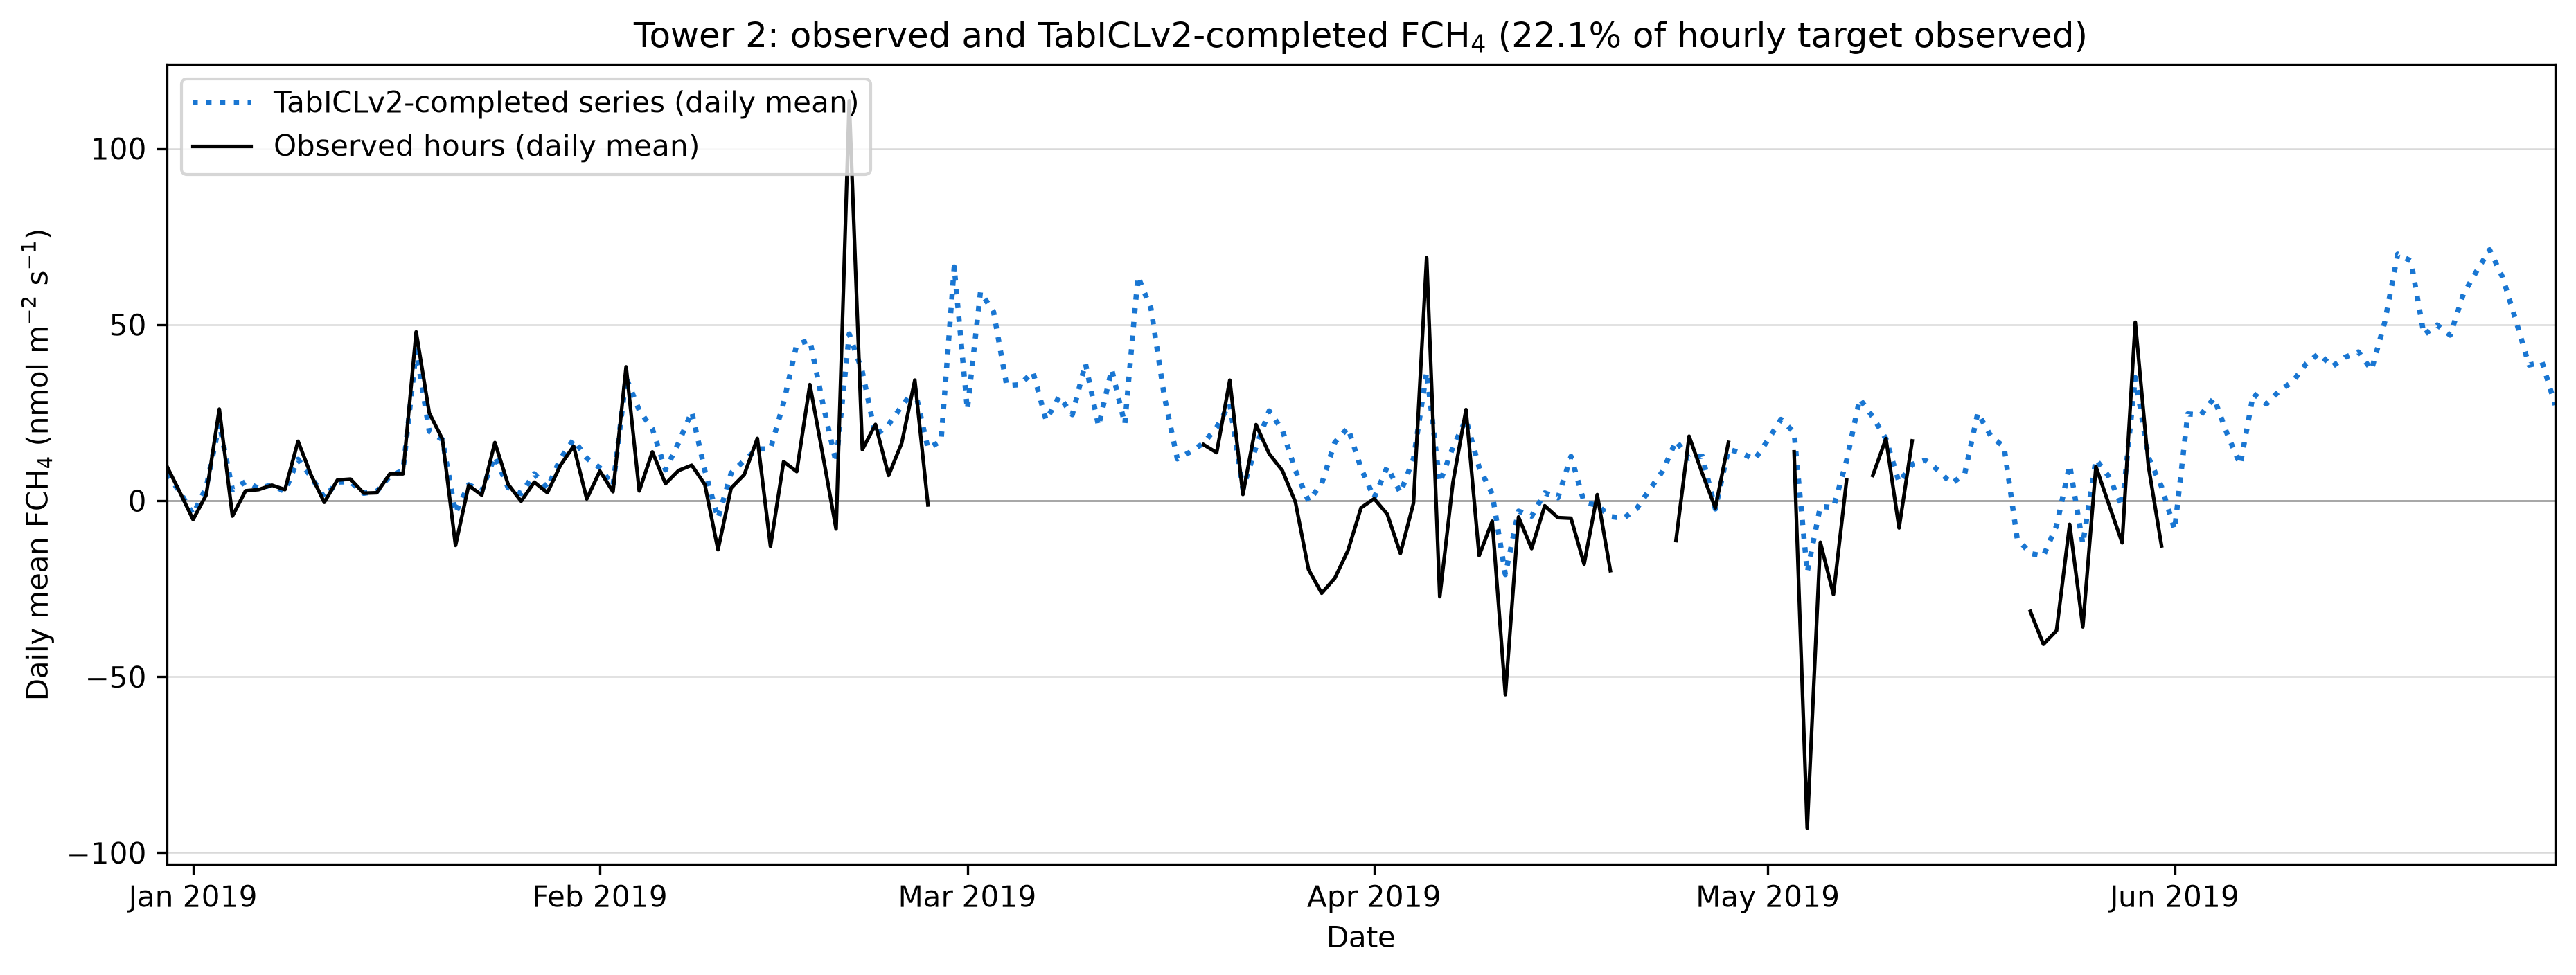
\includegraphics[width=\textwidth]{Figures/ch4_tabiclv2_daily_T2_2019H1.png}
\vspace{0.5em}

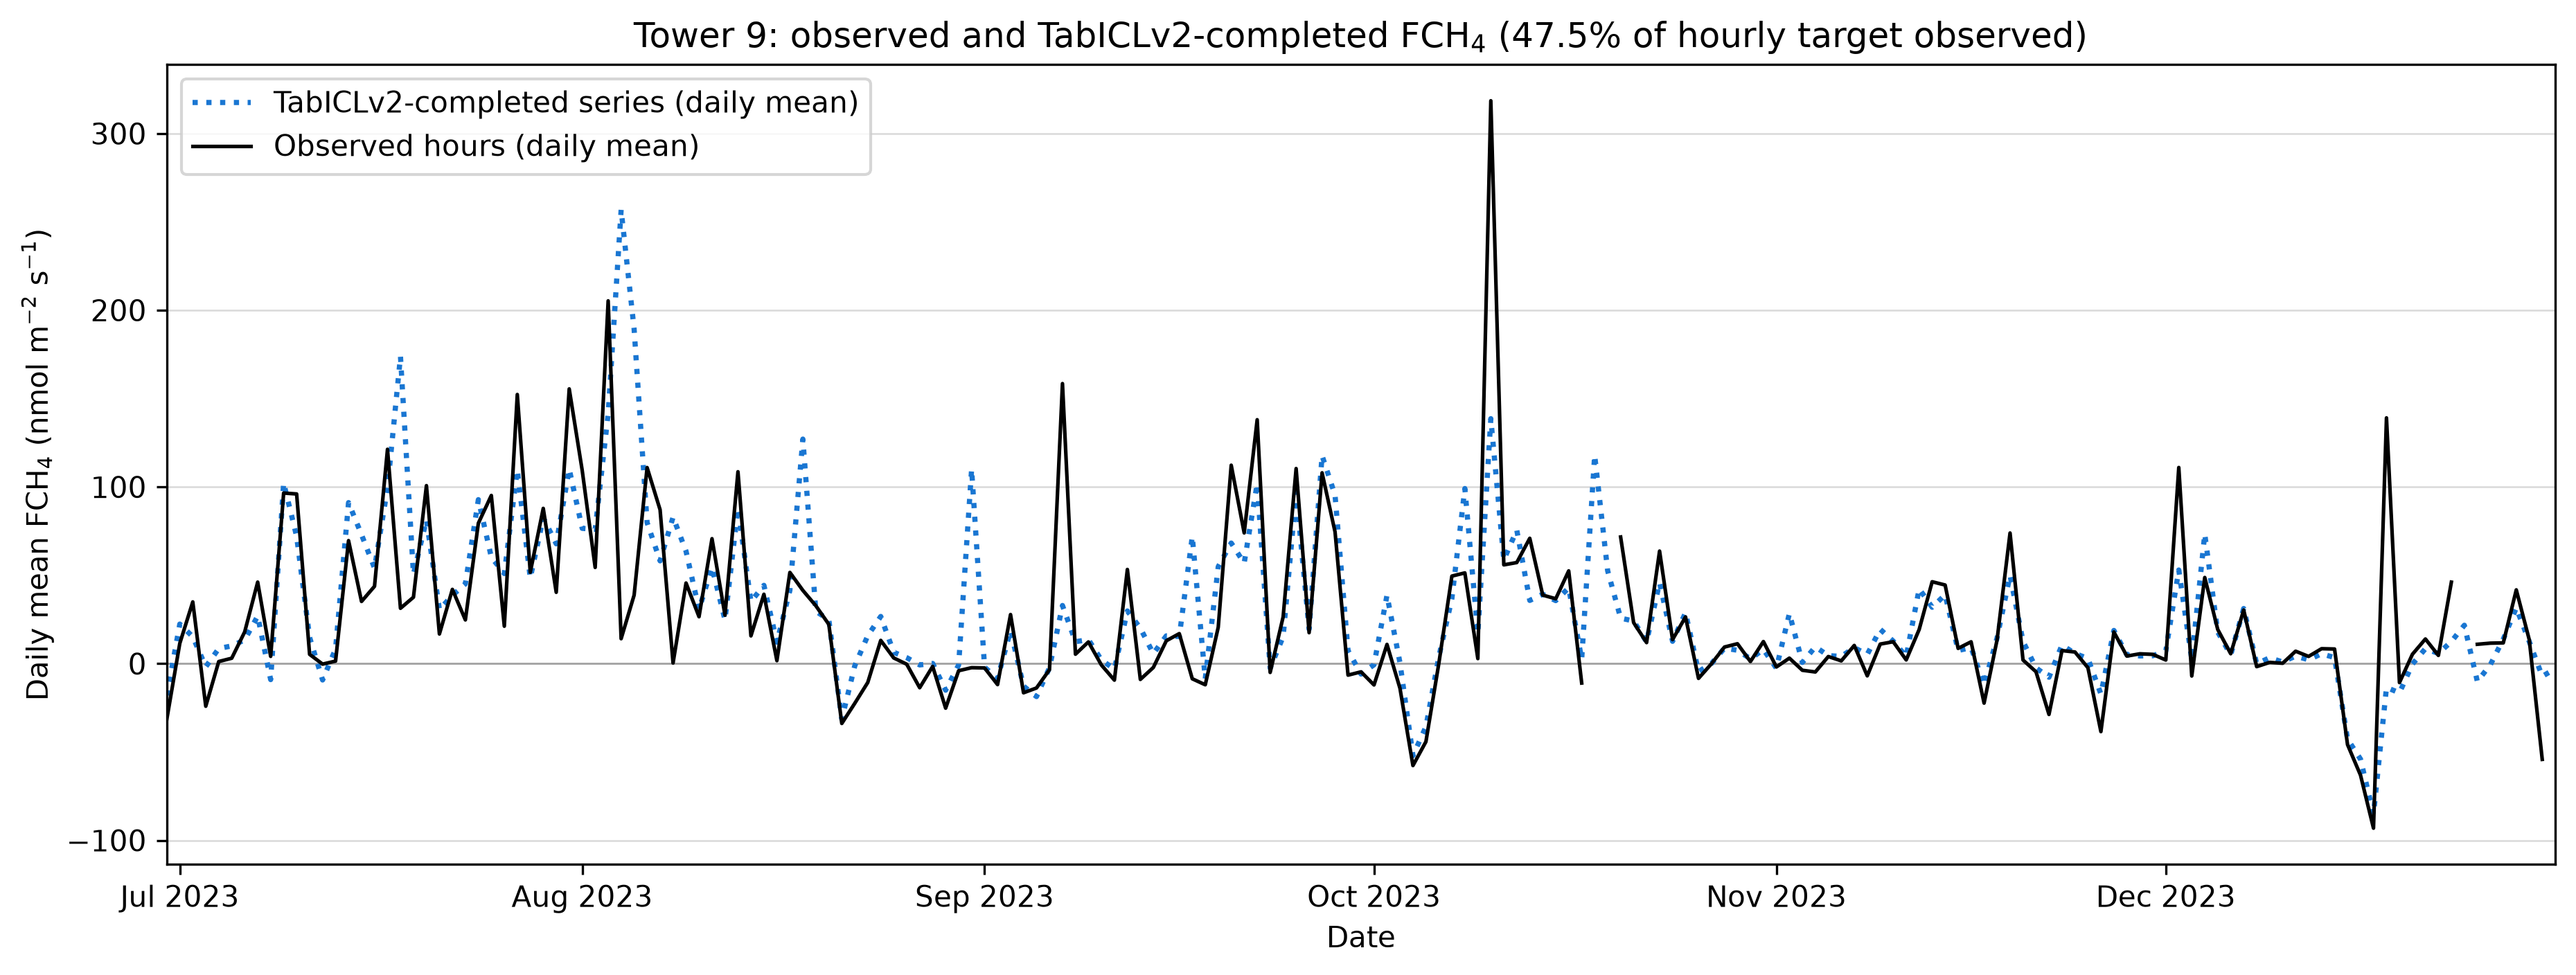
\includegraphics[width=\textwidth]{Figures/ch4_tabiclv2_daily_T9_2023H2.png}
\caption{Daily means from QC-valid observed hours (solid black) and the
TabICLv2-completed series (dotted blue) at T2 during January--June 2019 (top)
and T9 during July--December 2023 (bottom). Hourly target availability was
22.1\% at T2 and 47.5\% at T9. The completed series preserves observations and
fills missing hours with TabICLv2 estimates; the panels are reconstruction
diagnostics rather than held-out validation. The corresponding T4 example is
shown in Figure~\ref{fig:gf_t4_reconstruction}.}
\label{fig:app_gf_tabicl_daily_t2_t9}
\end{figure}

\begin{figure}[p]
\centering
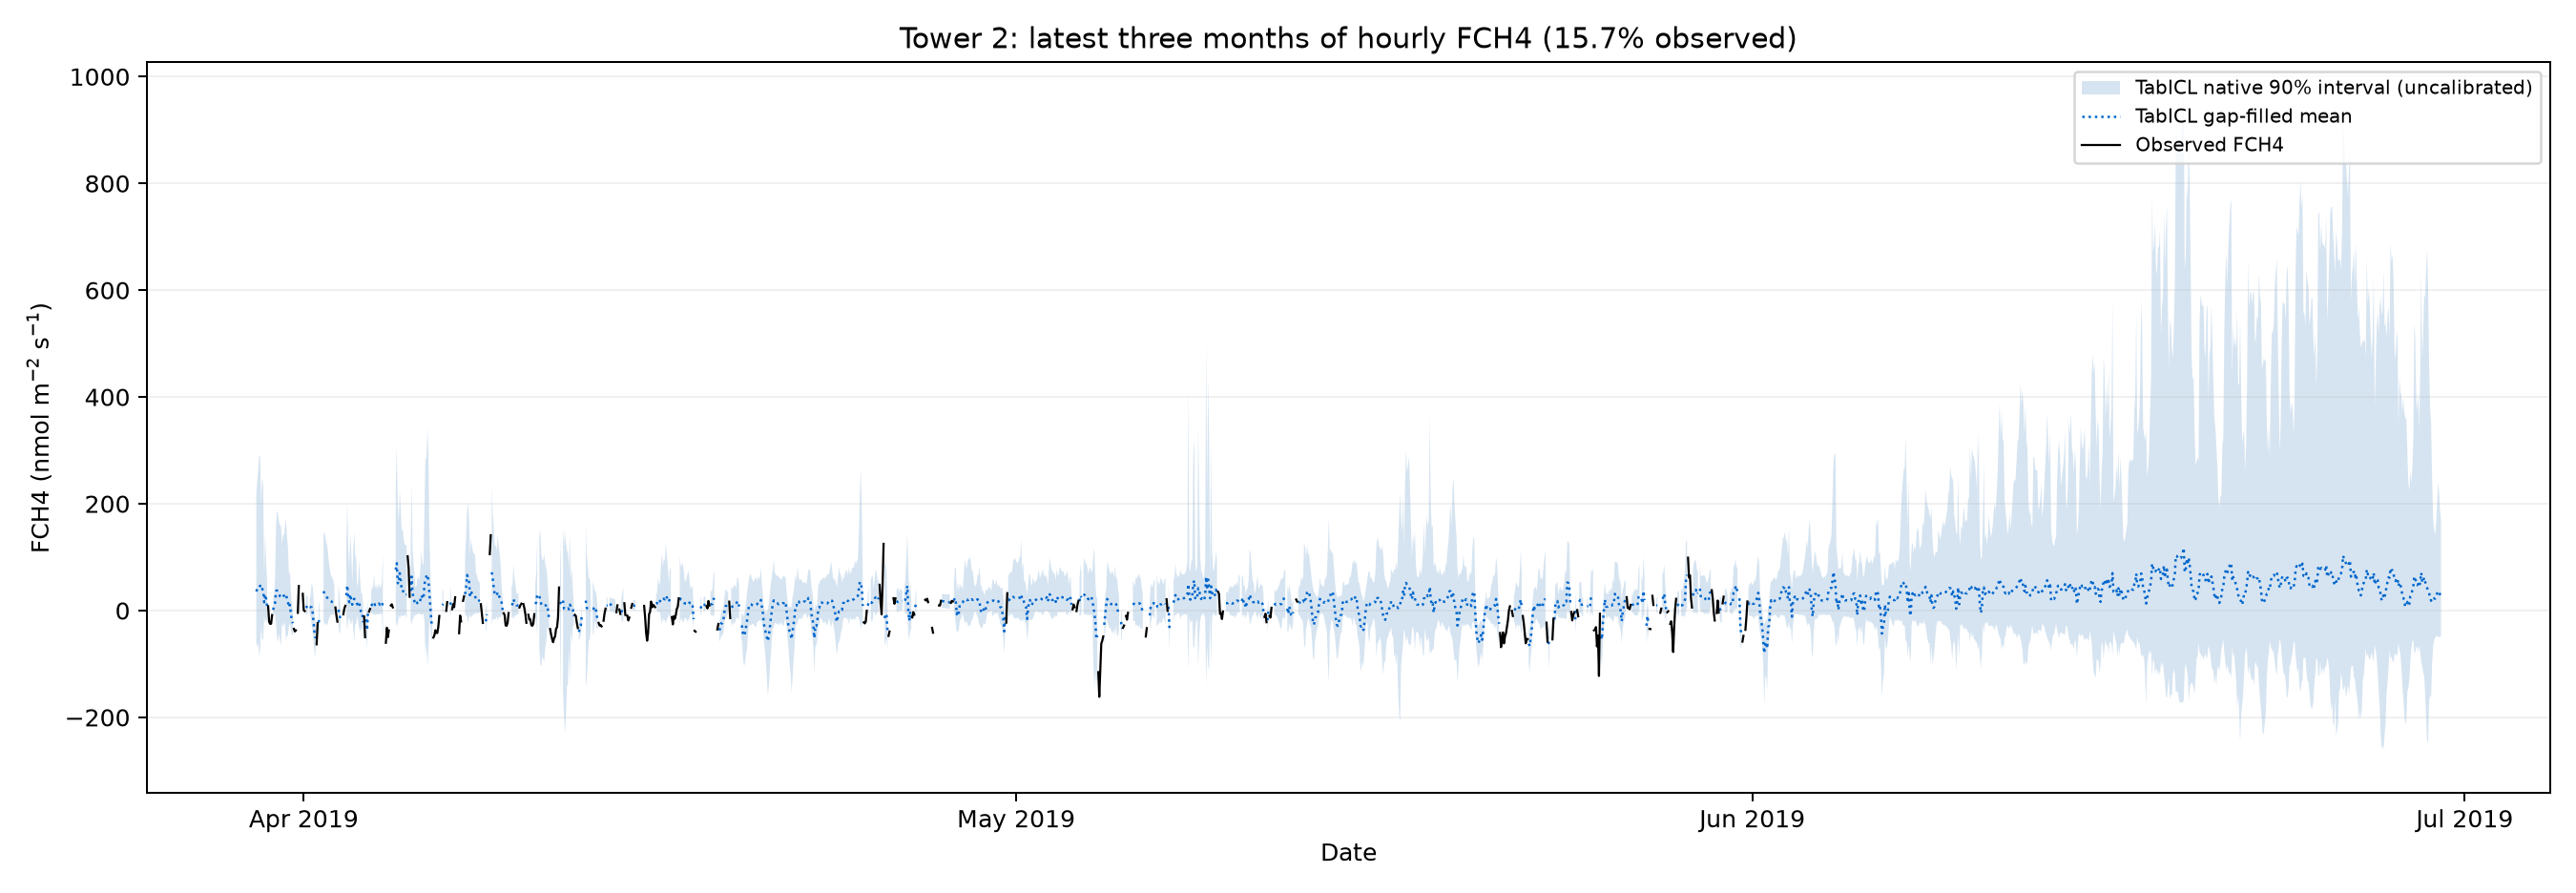
\includegraphics[width=\textwidth]{Figures/ch4_latest_tabicl_uq_hourly_T2_3month_example.png}
\vspace{0.5em}

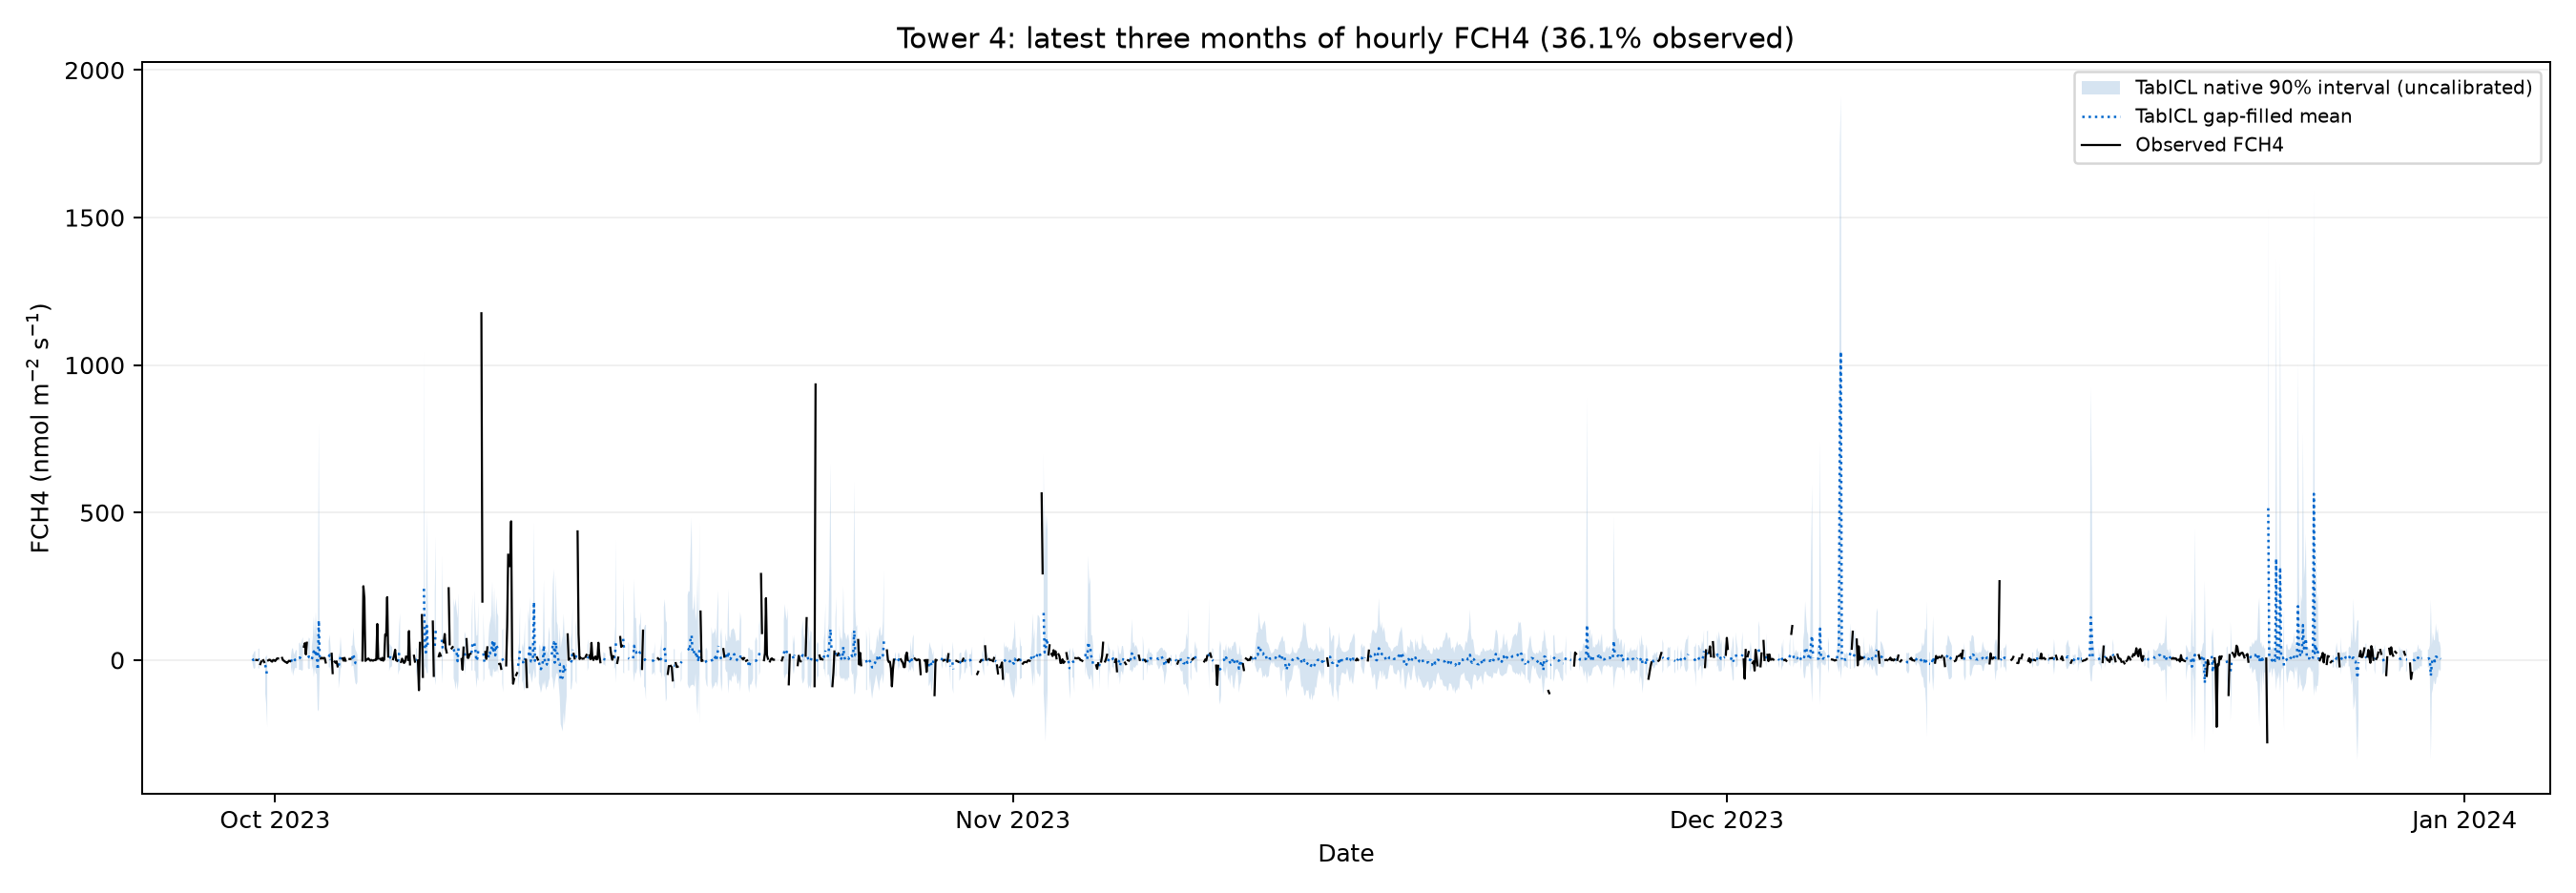
\includegraphics[width=\textwidth]{Figures/ch4_latest_tabicl_uq_hourly_T4_3month_example.png}
\caption{Three-month examples of hourly FCH\textsubscript{4} reconstruction
and native uncertainty for T2 (top) and T4 (bottom). Black lines show QC-valid
observations, dotted blue lines show the TabICLv2 gap-filled mean, and shaded
regions show the uncalibrated native 90\% interval. Each tower uses its latest
available three-month window and its own vertical scale.}
\label{fig:app_gf_tabicl_t2_t4}
\end{figure}

\FloatBarrier


\chapter{Forecasting}
\label{app:forecasting}

% % NEW
%   \subsection{Foundation-Model Forecasting Configurations}
%   \label{app:foundation-configurations}

%   \begin{table}[htbp]
%   \centering
%   \footnotesize
%   \renewcommand{\arraystretch}{1.15}
%   \begin{tabularx}{\textwidth}{
%   >{\raggedright\arraybackslash}p{0.19\textwidth}
%   >{\raggedright\arraybackslash}X
%   >{\raggedright\arraybackslash}X}
%   \toprule
%   Setting & TabPFN & TabICLv2 \\
%   \midrule

%   Implementation &
%   \texttt{tabpfn} 8.0.8; generic
%   \texttt{tabpfn-v2-regressor.ckpt} &
%   \texttt{tabicl} 2.1.1; default TabICLv2 regression weights \\

%   Estimator &
%   \texttt{TabPFNRegressor}, eight estimators, seed 137 &
%   \texttt{TabICLRegressor}, eight estimators, seed 42 \\

%   Training scope &
%   Pooled across T2, T4 and T9, with tower indicators &
%   Pooled across T2, T4 and T9, with tower indicators \\

%   Predictors &
%   The 57 predictors listed in Table~\ref{tab:fc_tabpfn_features} &
%   The same 57-predictor frame \\

%   Target observations &
%   QC-valid pre-origin \texttt{y\_observed} only &
%   QC-valid pre-origin \texttt{y\_observed} only \\

%   Missing predictors &
%   Training-set mean imputation &
%   Training-set mean imputation \\

%   Context &
%   Equal-weight combination of an all-history spike-corrected model,
%   a 1,095-day model and a 1,460-day model &
%   Most recent 1,460 days \\

%   Target processing &
%   Raw target for the all-history and 1,095-day components; tower-wise
%   median/IQR normalisation for the 1,460-day component &
%   Tower-wise median/IQR normalisation \\

%   Point estimate &
%   Predictive median &
%   Predictive median \\

%   Final prediction &
%   Arithmetic mean of the three component forecasts &
%   Single-model prediction; exploratory ensembles were not retained \\

%   \bottomrule
%   \end{tabularx}
%   \caption{Implementation settings for the B18 tabular-foundation-model
%   forecasting experiments. All preprocessing statistics and event thresholds
%   were estimated from pre-origin training data only.}
%   \label{tab:app_foundation_configurations}
%   \end{table}

\begin{figure}[htbp]
\centering
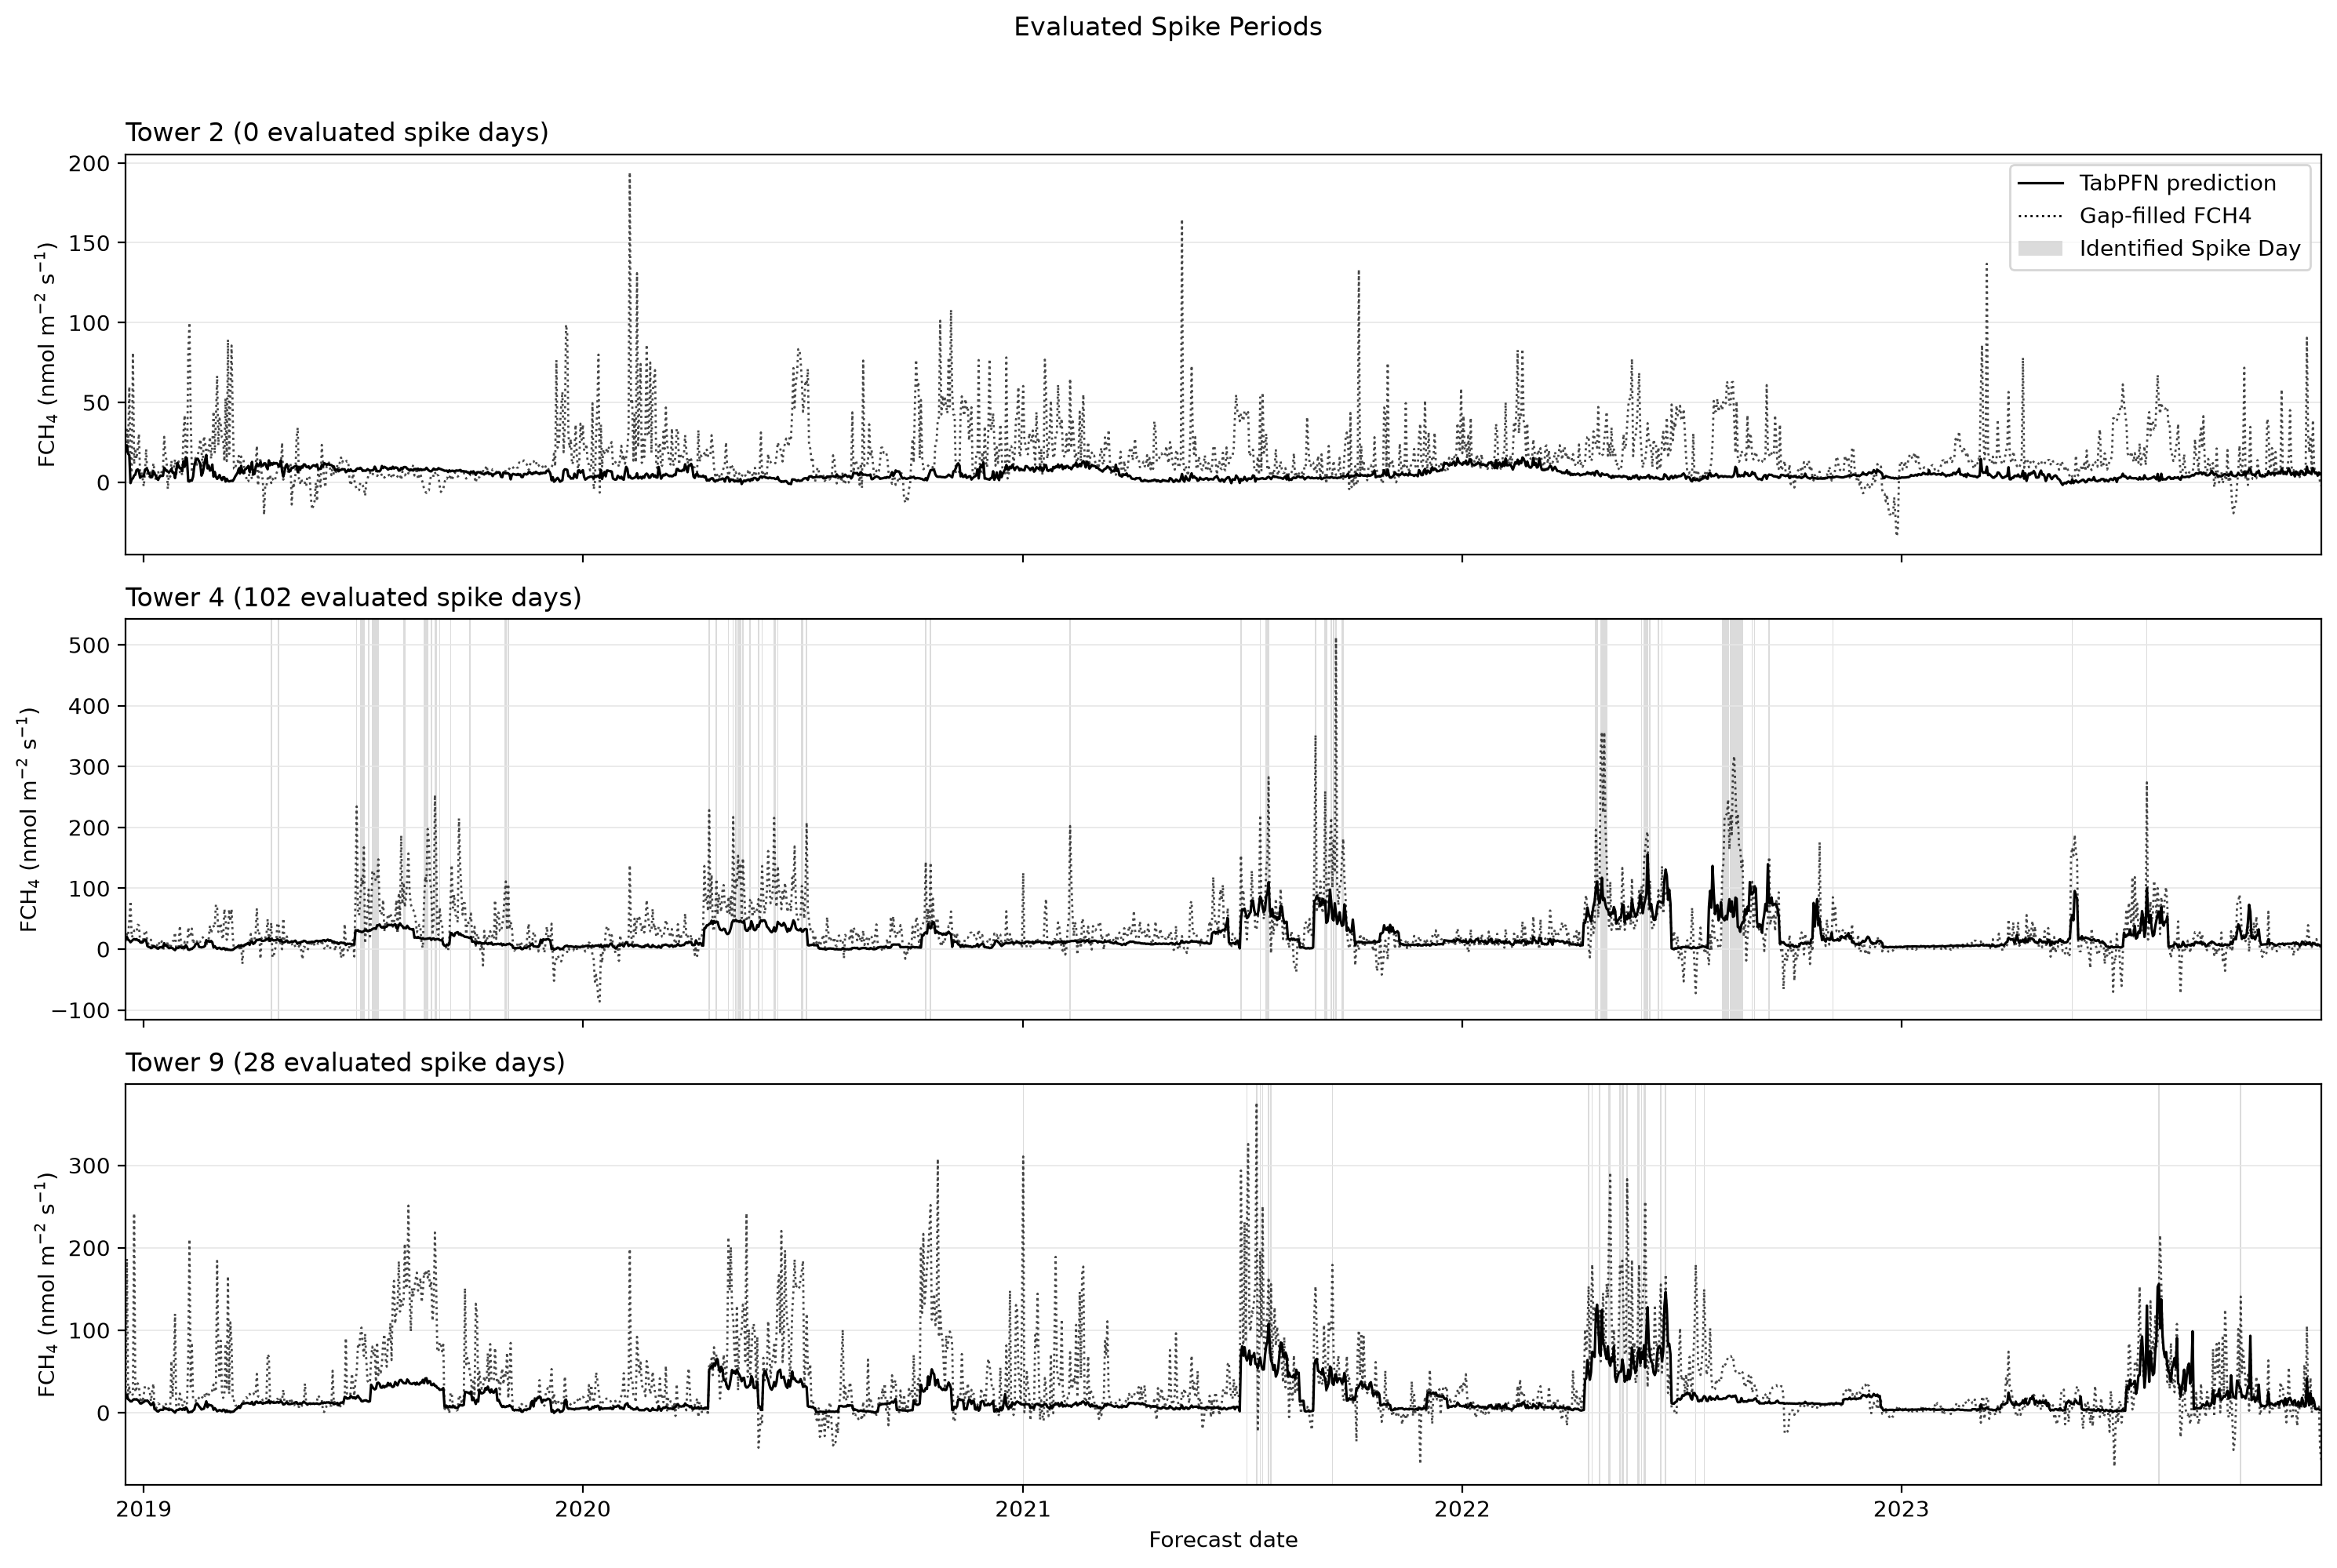
\includegraphics[width=\textwidth]{Figures/ch5_B18_p95_spike_timing_all_towers.png}
\caption{Temporal distribution of the spike observations used in the
forecasting evaluation. Grey bands mark QC-valid observations above the
tower- and origin-specific pre-forecast 95th-percentile threshold; the solid
line shows the TabPFN prediction and the dotted line
shows the gap-filled FCH\textsubscript{4} series for context. The evaluated
sample contains no spike days at T2, 102 at T4 and 28 at T9.}
\label{fig:app_fc_spike_timing}
\end{figure}

\begin{figure}[htbp]
\centering
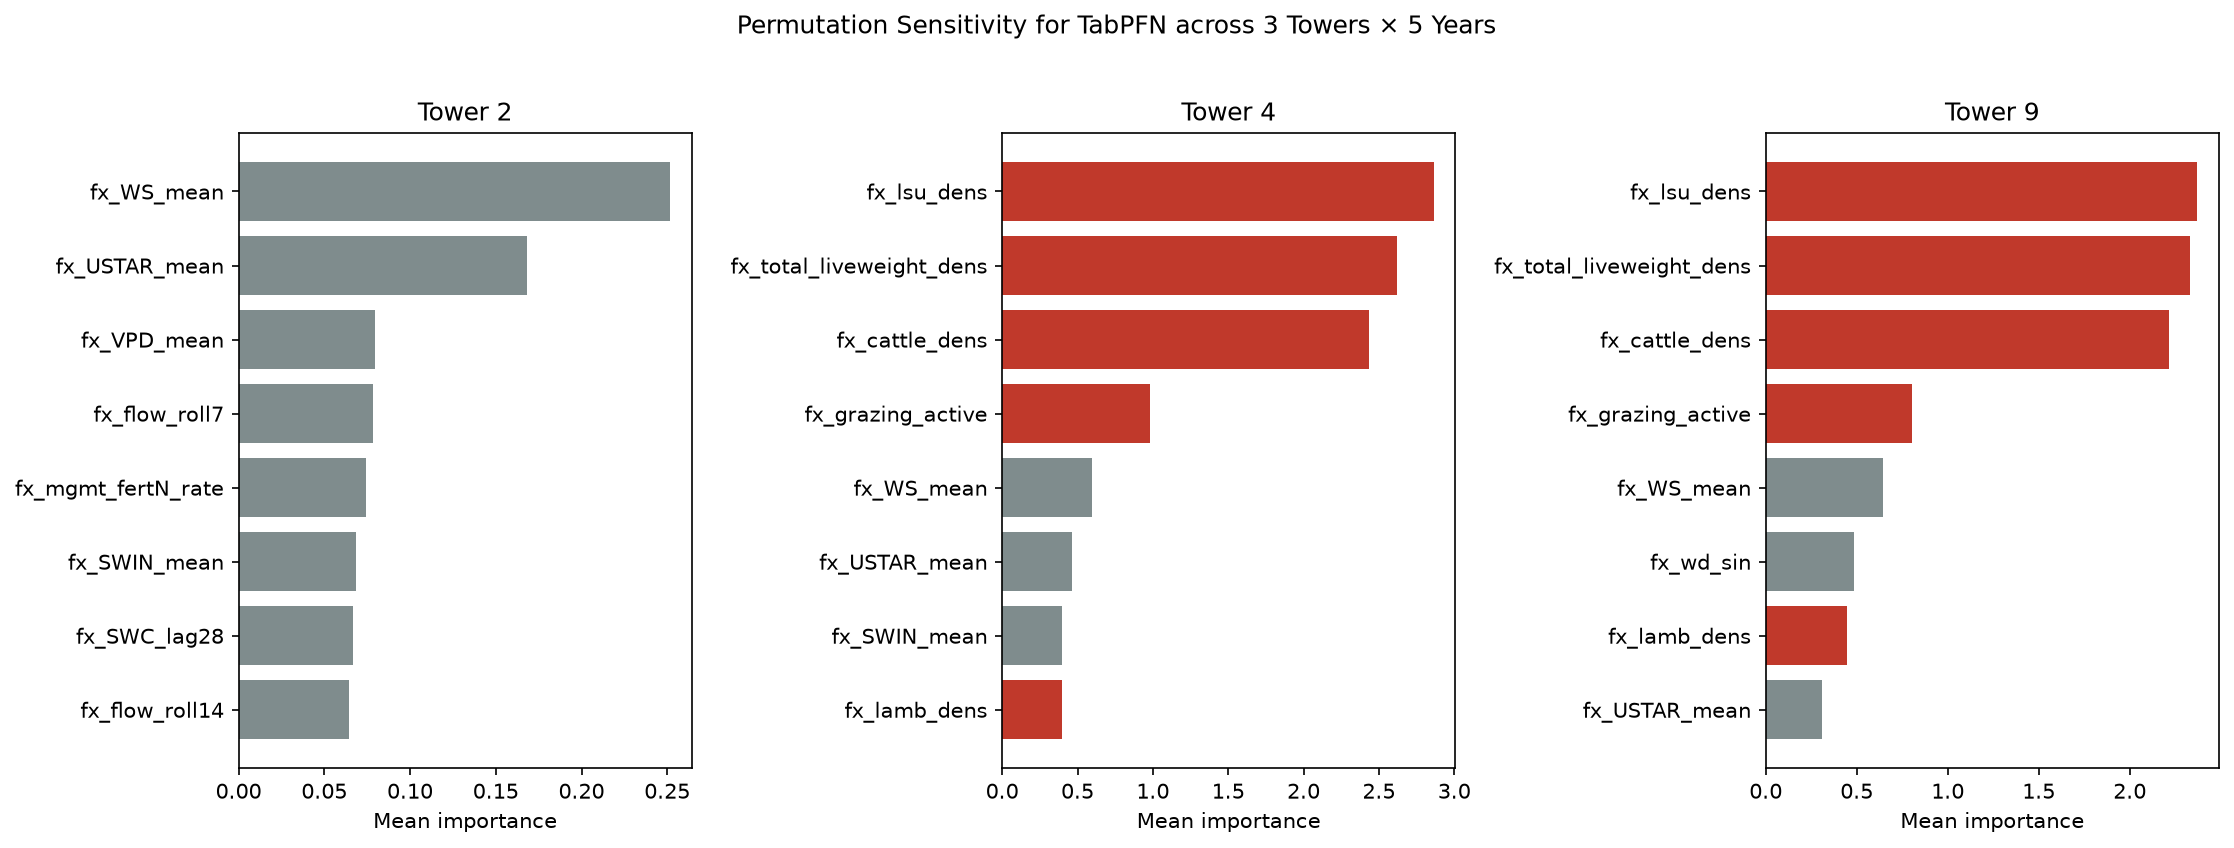
\includegraphics[width=\textwidth]{Figures/ch5_tabpfn_permutation_sensitivity_by_tower.png}
\caption{Tower-specific permutation-sensitivity rankings for the TabPFN
model. The figure shows the leading predictors
within T2, T4 and T9, complementing the pooled ranking in
Figure~\ref{fig:fc_tabpfn_importance}.}
\label{fig:app_fc_importance_by_tower}
\end{figure}

\begin{figure}[htbp]
\centering
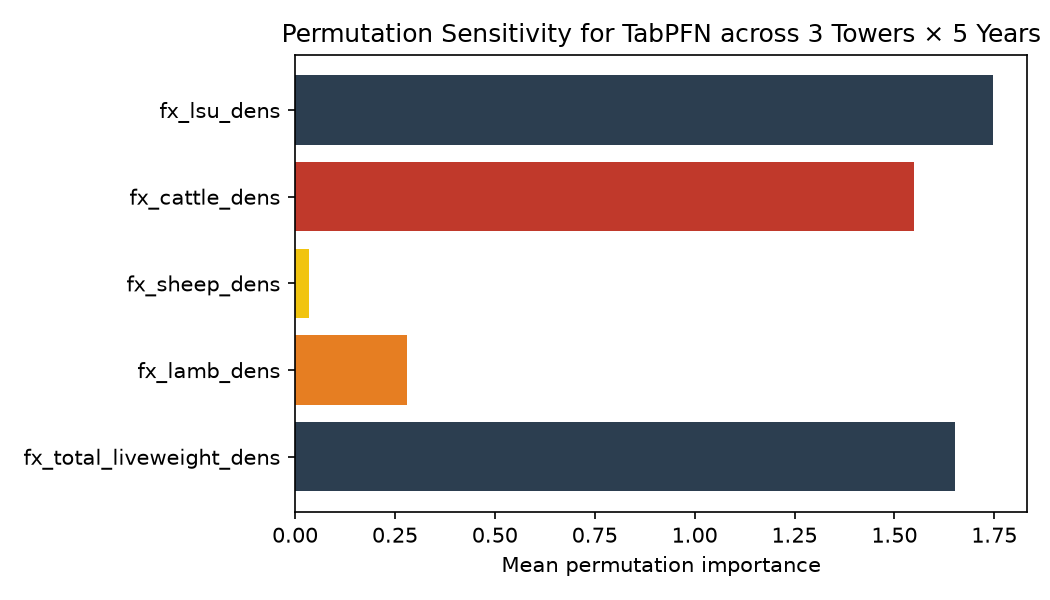
\includegraphics[width=0.75\textwidth]{Figures/ch5_tabpfn_permutation_sensitivity_species.png}
\caption{Permutation sensitivity of the livestock-species predictors in the
TabPFN model. The comparison separates the
contributions of cattle, sheep and lamb density within the broader livestock
signal.}
\label{fig:app_fc_importance_species}
\end{figure}

\begin{figure}[htbp]
\centering
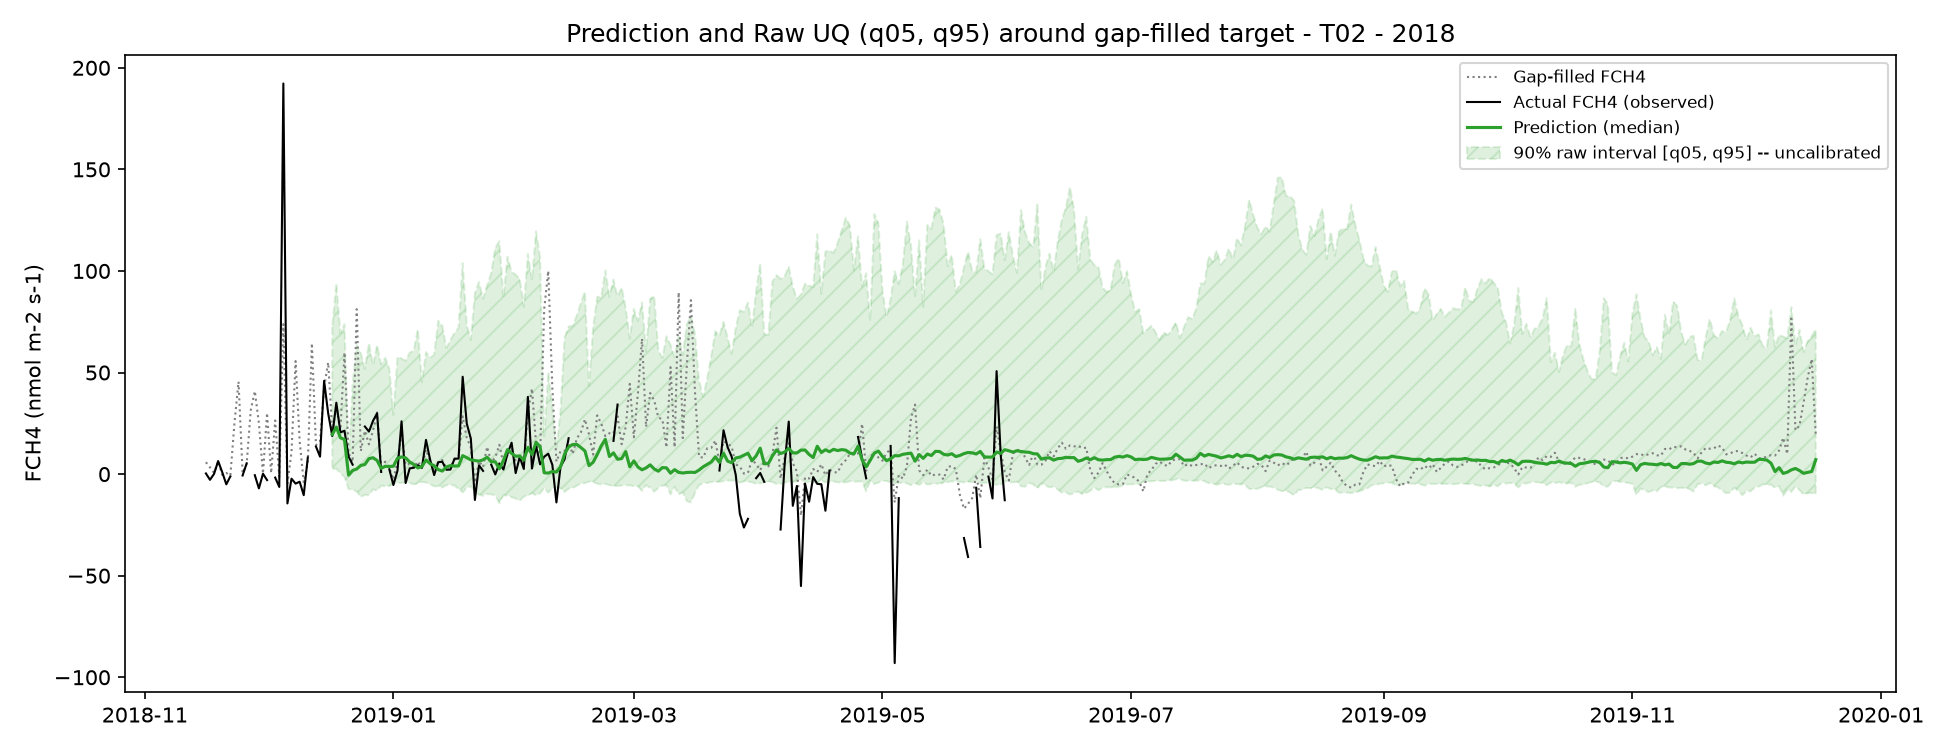
\includegraphics[width=\textwidth]{Figures/cqr_gallery/ch5_cqr_forecast_T02_2018.png}
\caption{Representative 365-day TabPFN forecast at T2 from the 2018 forecast
origin. The green line is the median forecast, the black line shows available
observations, and the dotted line provides the gap-filled series as context.
The hatched region is the native raw 90\% quantile interval. Conformal
calibration was not applied because the available T2 observations were
insufficient to construct a leave-one-origin-out calibration set.}
\label{fig:app_fc_uq_t2_raw}
\end{figure}

\begin{figure}[htbp]
\centering
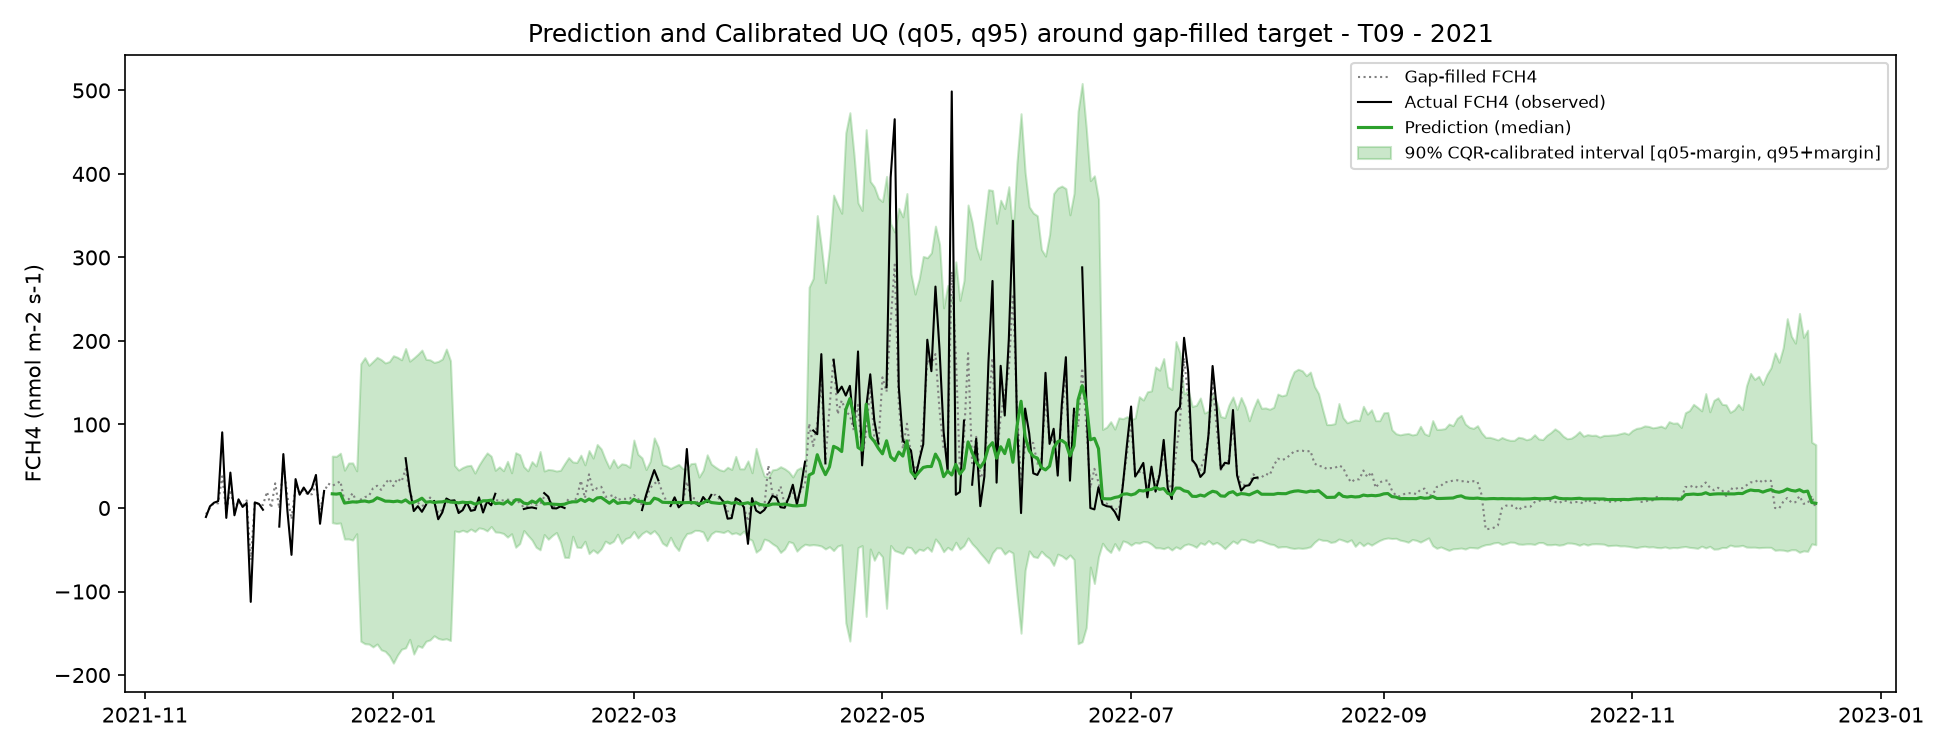
\includegraphics[width=\textwidth]{Figures/cqr_gallery/ch5_cqr_forecast_T09_2021.png}
\caption{Representative 365-day TabPFN forecast at T9 from the 2021 forecast
origin. The green line is the median forecast, the black line shows available
observations, the dotted line provides the gap-filled series as context, and
the shaded region is the 90\% CQR-calibrated prediction interval across the
complete forecast horizon.}
\label{fig:app_fc_cqr_t9}
\end{figure}

\FloatBarrier


\chapter{Scenario Projection}
\label{app:scenario-projection}

\begin{figure}[htbp]
\centering
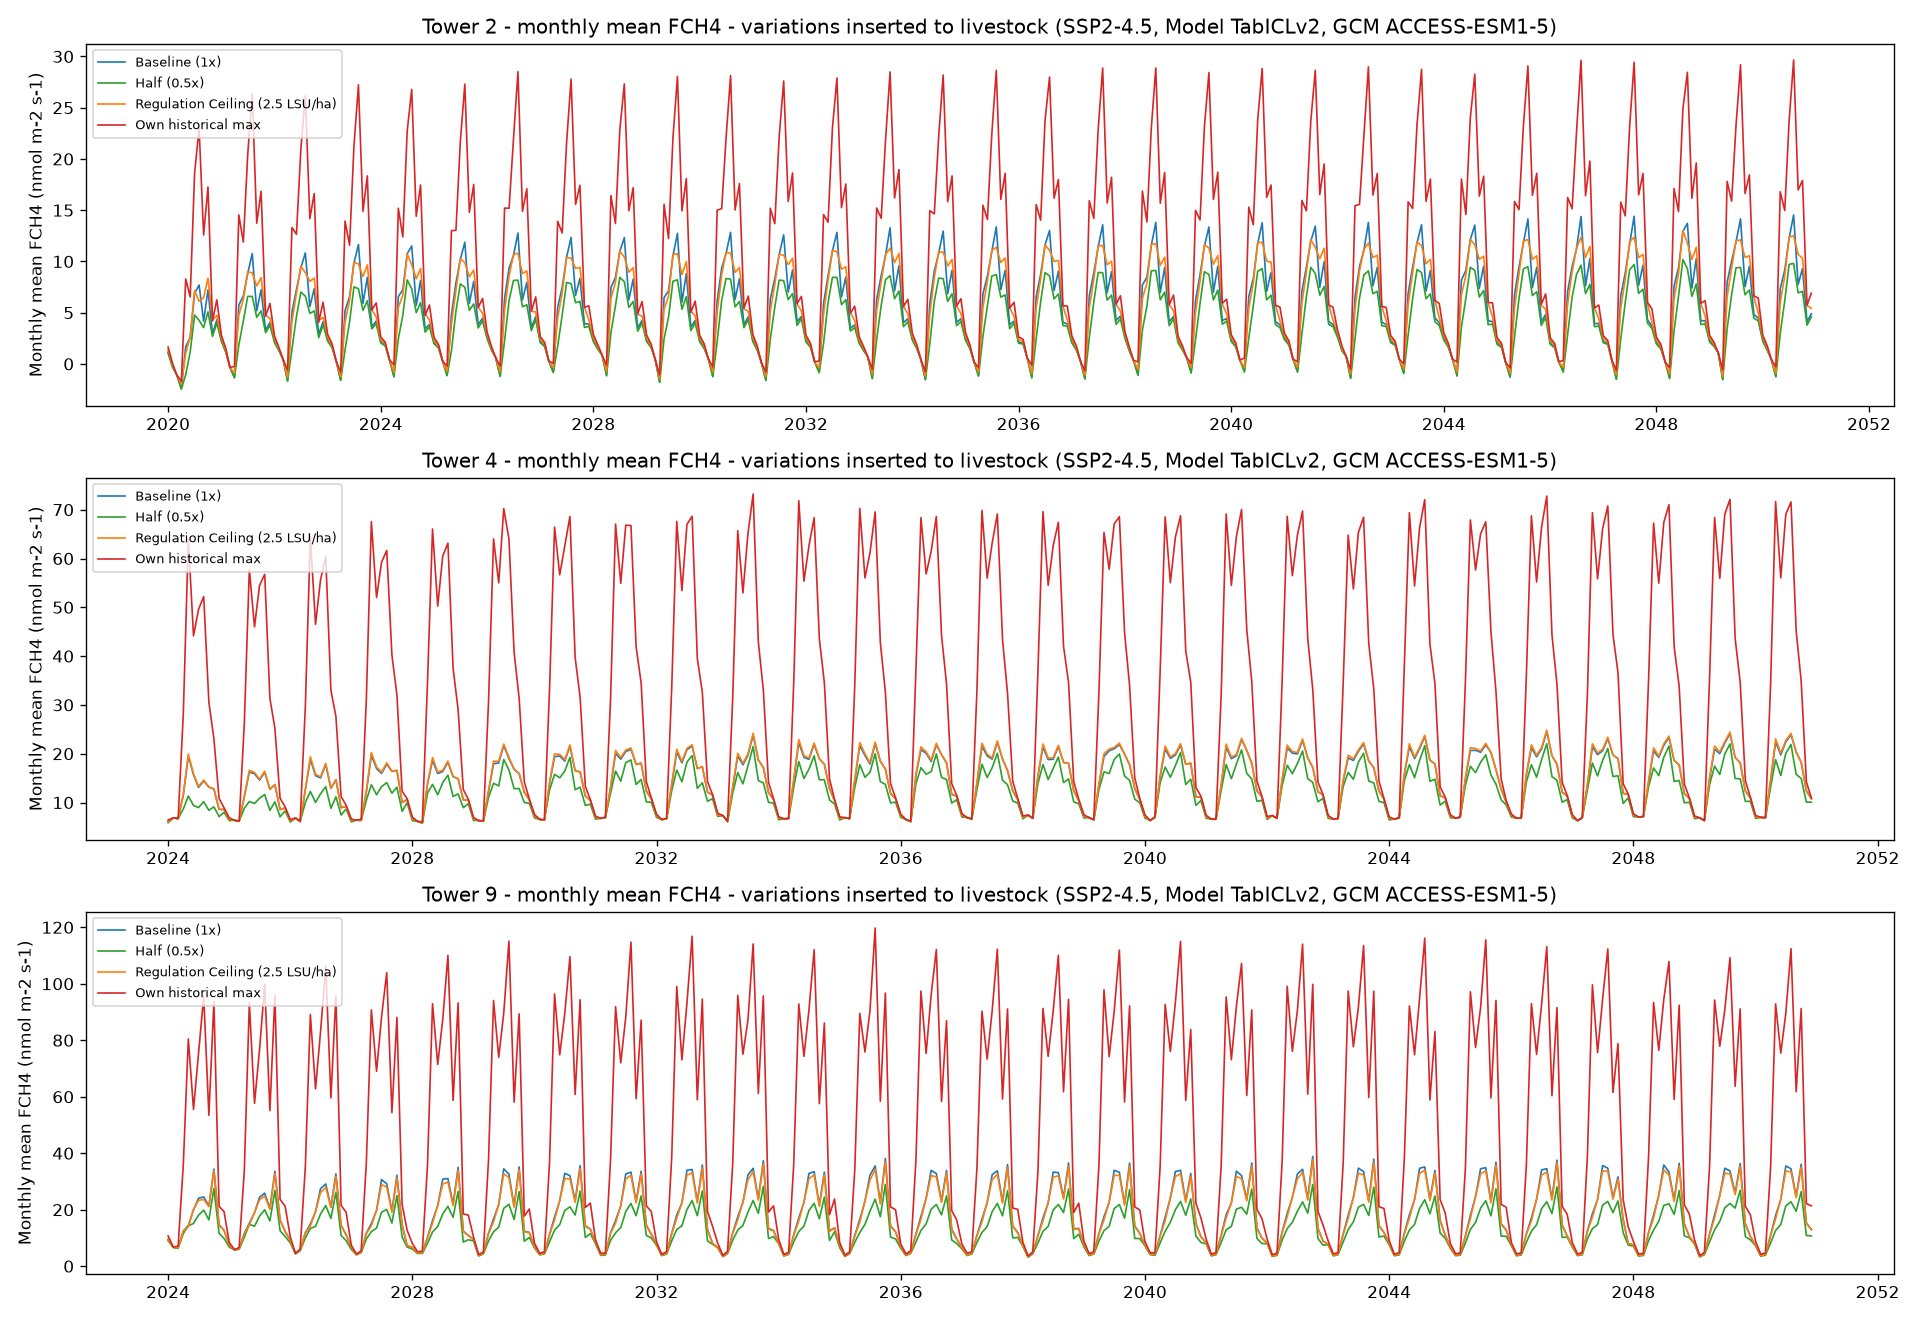
\includegraphics[width=\textwidth]{Figures/ch6_livestock_ladder_trajectory_ssp245.png}
\caption{Monthly mean FCH\textsubscript{4} (nmol~m\textsuperscript{-2}~s\textsuperscript{-1}) at T2, T4 and T9 under SSP2-4.5 for the livestock-density ladder -- baseline, half-density,
government-reference and own-historical-maximum (all-species) -- for a single illustrative
trajectory (restricted model, GCM ACCESS-ESM1-5, realisation~1). Table~\ref{tab:livestock_scenario_results}
reports the mean annual percentage change, averaged across all five GCMs and ten realisations per
GCM.}
\label{fig:app_sp_livestock_trajectory_ssp245}
\end{figure}

\begin{figure}[htbp]
\centering
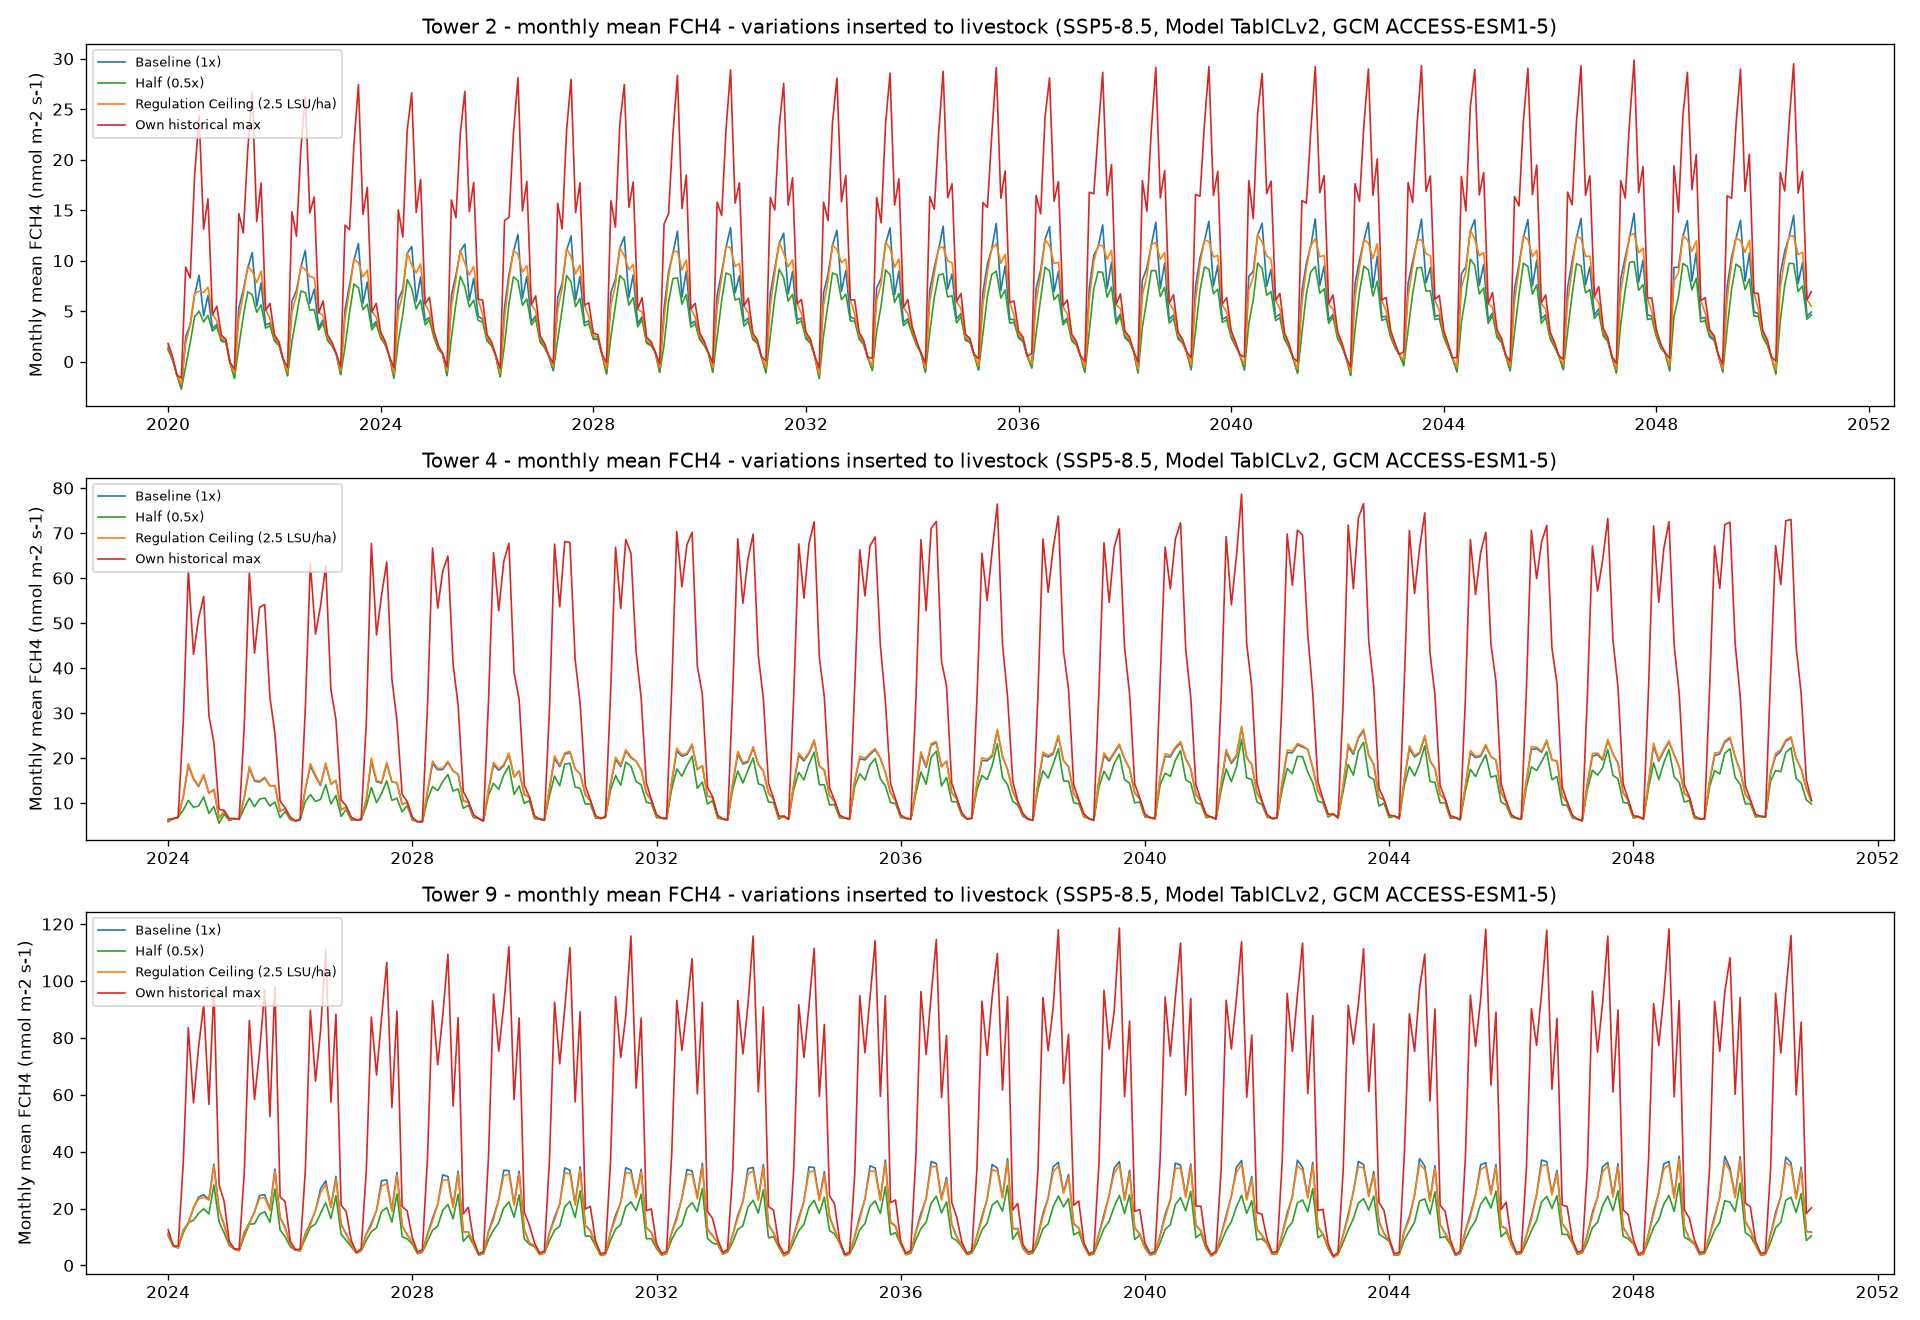
\includegraphics[width=\textwidth]{Figures/ch6_livestock_ladder_trajectory_ssp585.png}
\caption{As Figure~\ref{fig:app_sp_livestock_trajectory_ssp245}, under SSP5-8.5. The near-identical
trajectories under both pathways illustrate Table~\ref{tab:livestock_scenario_results}'s finding
that the SSP pathway itself makes almost no difference to the livestock-density response.}
\label{fig:app_sp_livestock_trajectory_ssp585}
\end{figure}

\FloatBarrier

\begin{figure}[htbp]
\centering
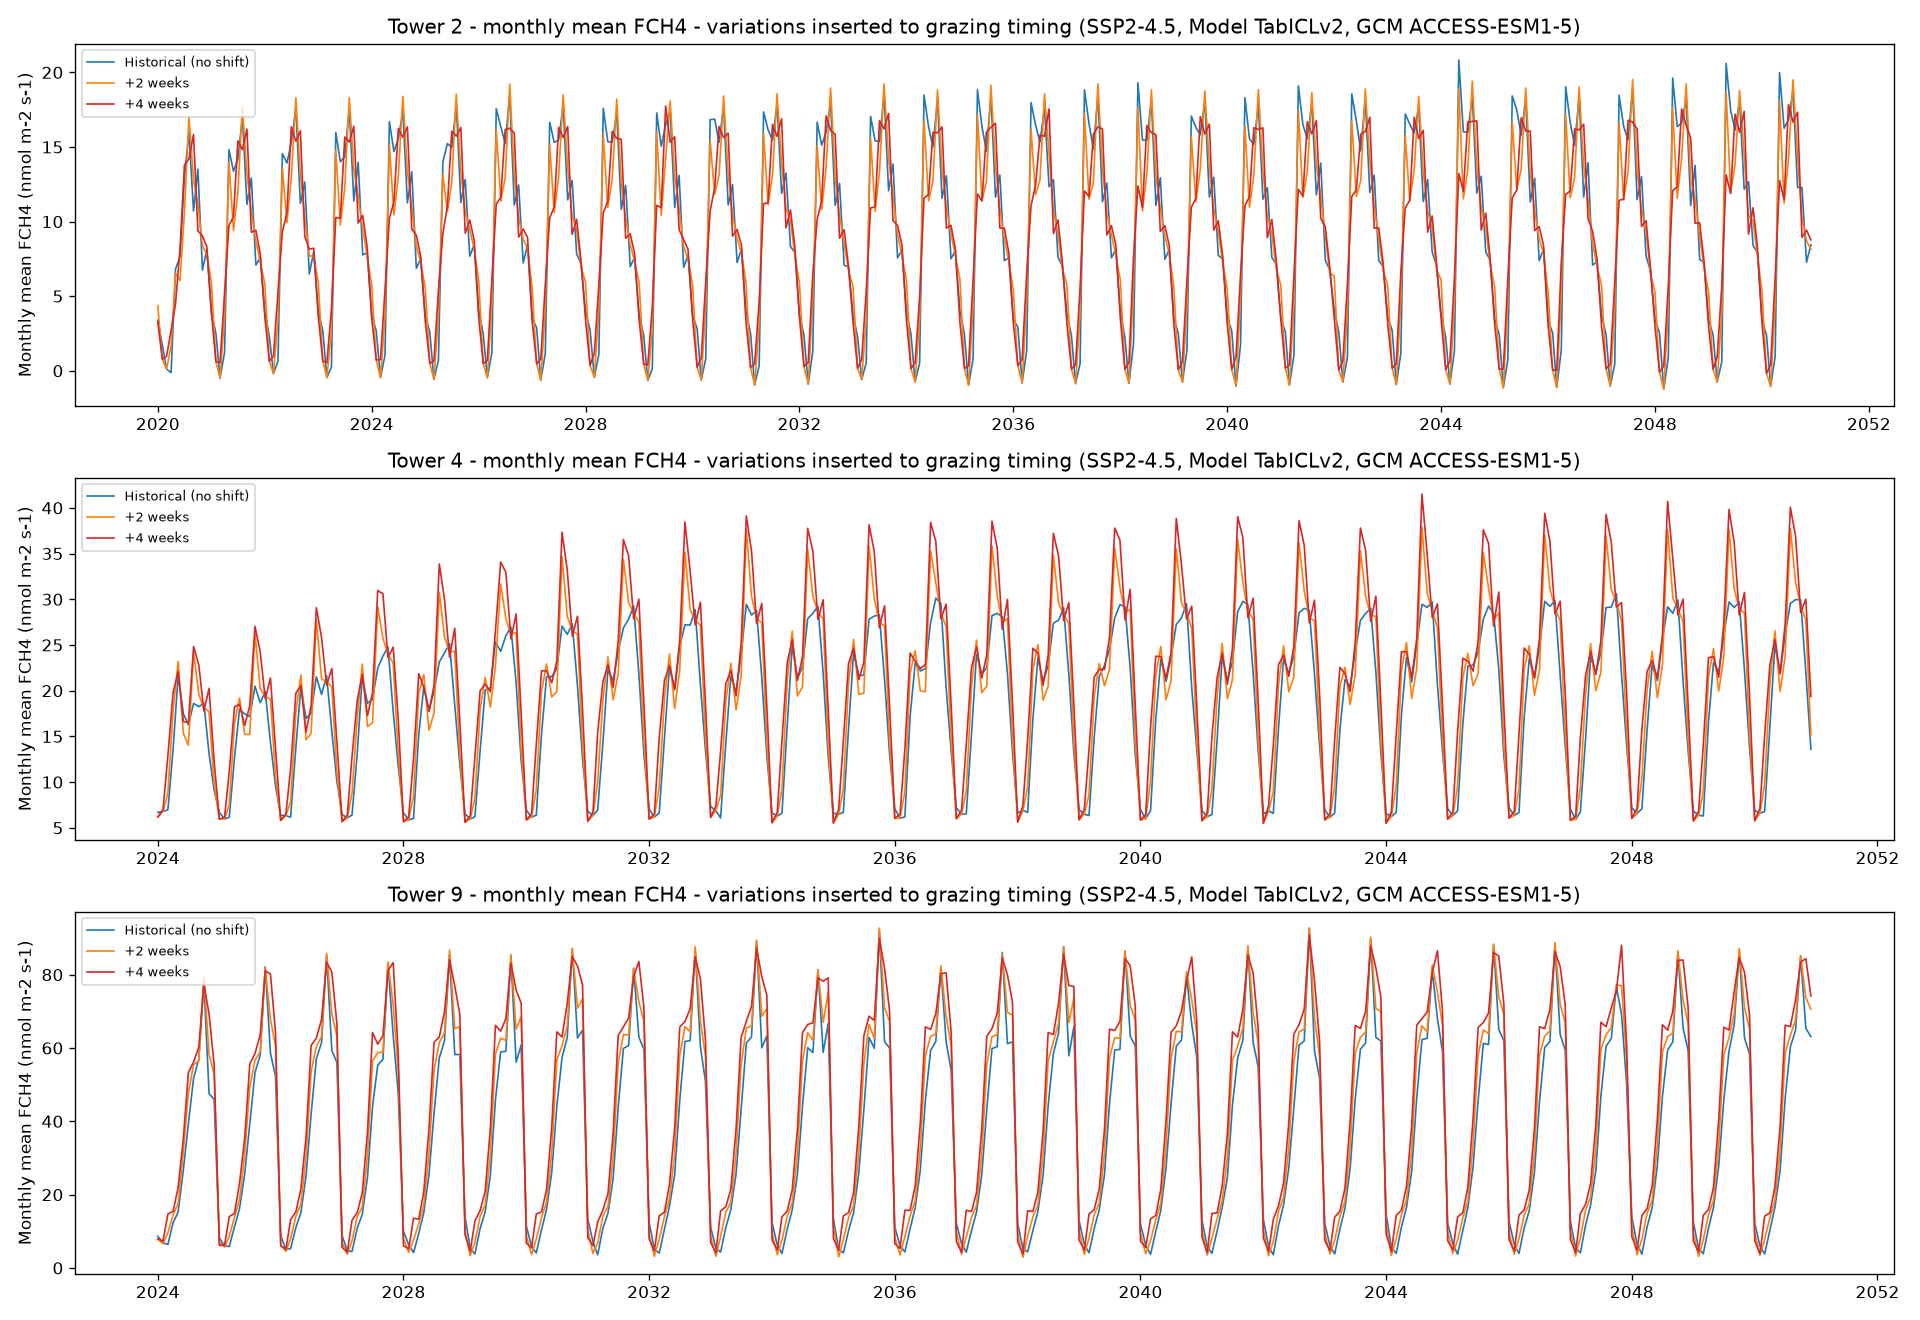
\includegraphics[width=\textwidth]{Figures/ch6_grazing_trajectory_ssp245.png}
\caption{Monthly mean FCH\textsubscript{4} (nmol~m\textsuperscript{-2}~s\textsuperscript{-1}) at T2, T4 and T9 under SSP2-4.5 for the historical grazing-timing baseline and its $+2$-week
and $+4$-week shift perturbations, for a single illustrative trajectory (restricted model, GCM
ACCESS-ESM1-5, realisation~1). Table~\ref{tab:management_scenario_results} reports the mean
annual percentage change for the $+4$-week shift only, averaged across all five GCMs and ten
realisations per GCM.}
\label{fig:app_sp_grazing_trajectory_ssp245}
\end{figure}

\begin{figure}[htbp]
\centering
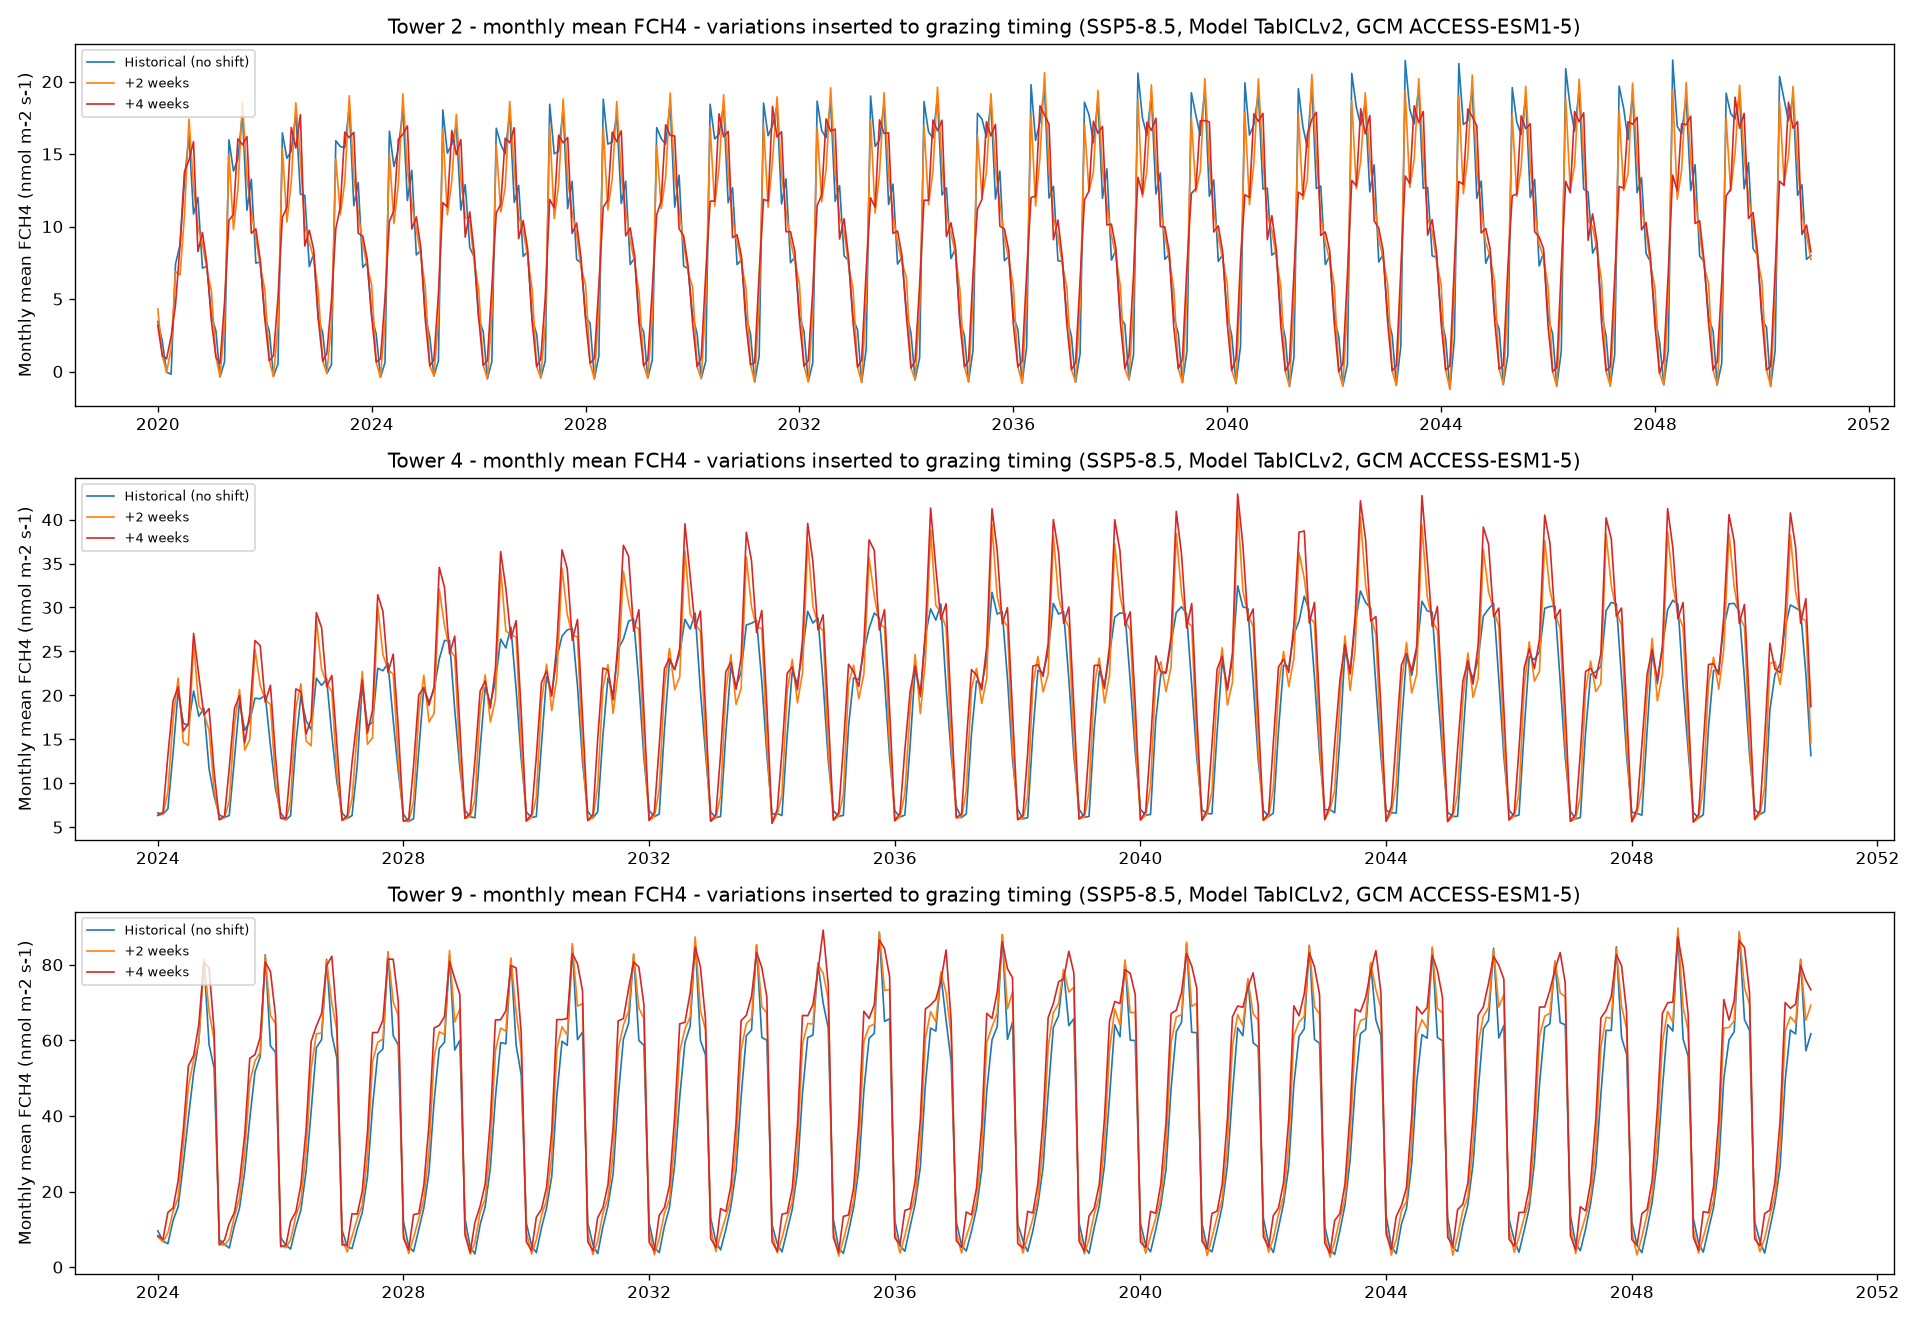
\includegraphics[width=\textwidth]{Figures/ch6_grazing_trajectory_ssp585.png}
\caption{
    Monthly mean FCH\textsubscript{4} (nmol~m\textsuperscript{-2}~s\textsuperscript{-1}) 
    at T2, T4 and T9 under SSP5-8.5 for the historical grazing-timing baseline and its
$+2$-week and $+4$-week shift perturbations, for a single illustrative trajectory
(restricted model, GCM ACCESS-ESM1-5, realisation~1). Table~\ref{tab:management_scenario_results} reports the mean
annual percentage change for the $+4$-week shift only, averaged across all five GCMs and ten
realisations per GCM.
}
\label{fig:app_sp_grazing_trajectory_ssp585}
\end{figure}

\FloatBarrier

\begin{figure}[htbp]
\centering
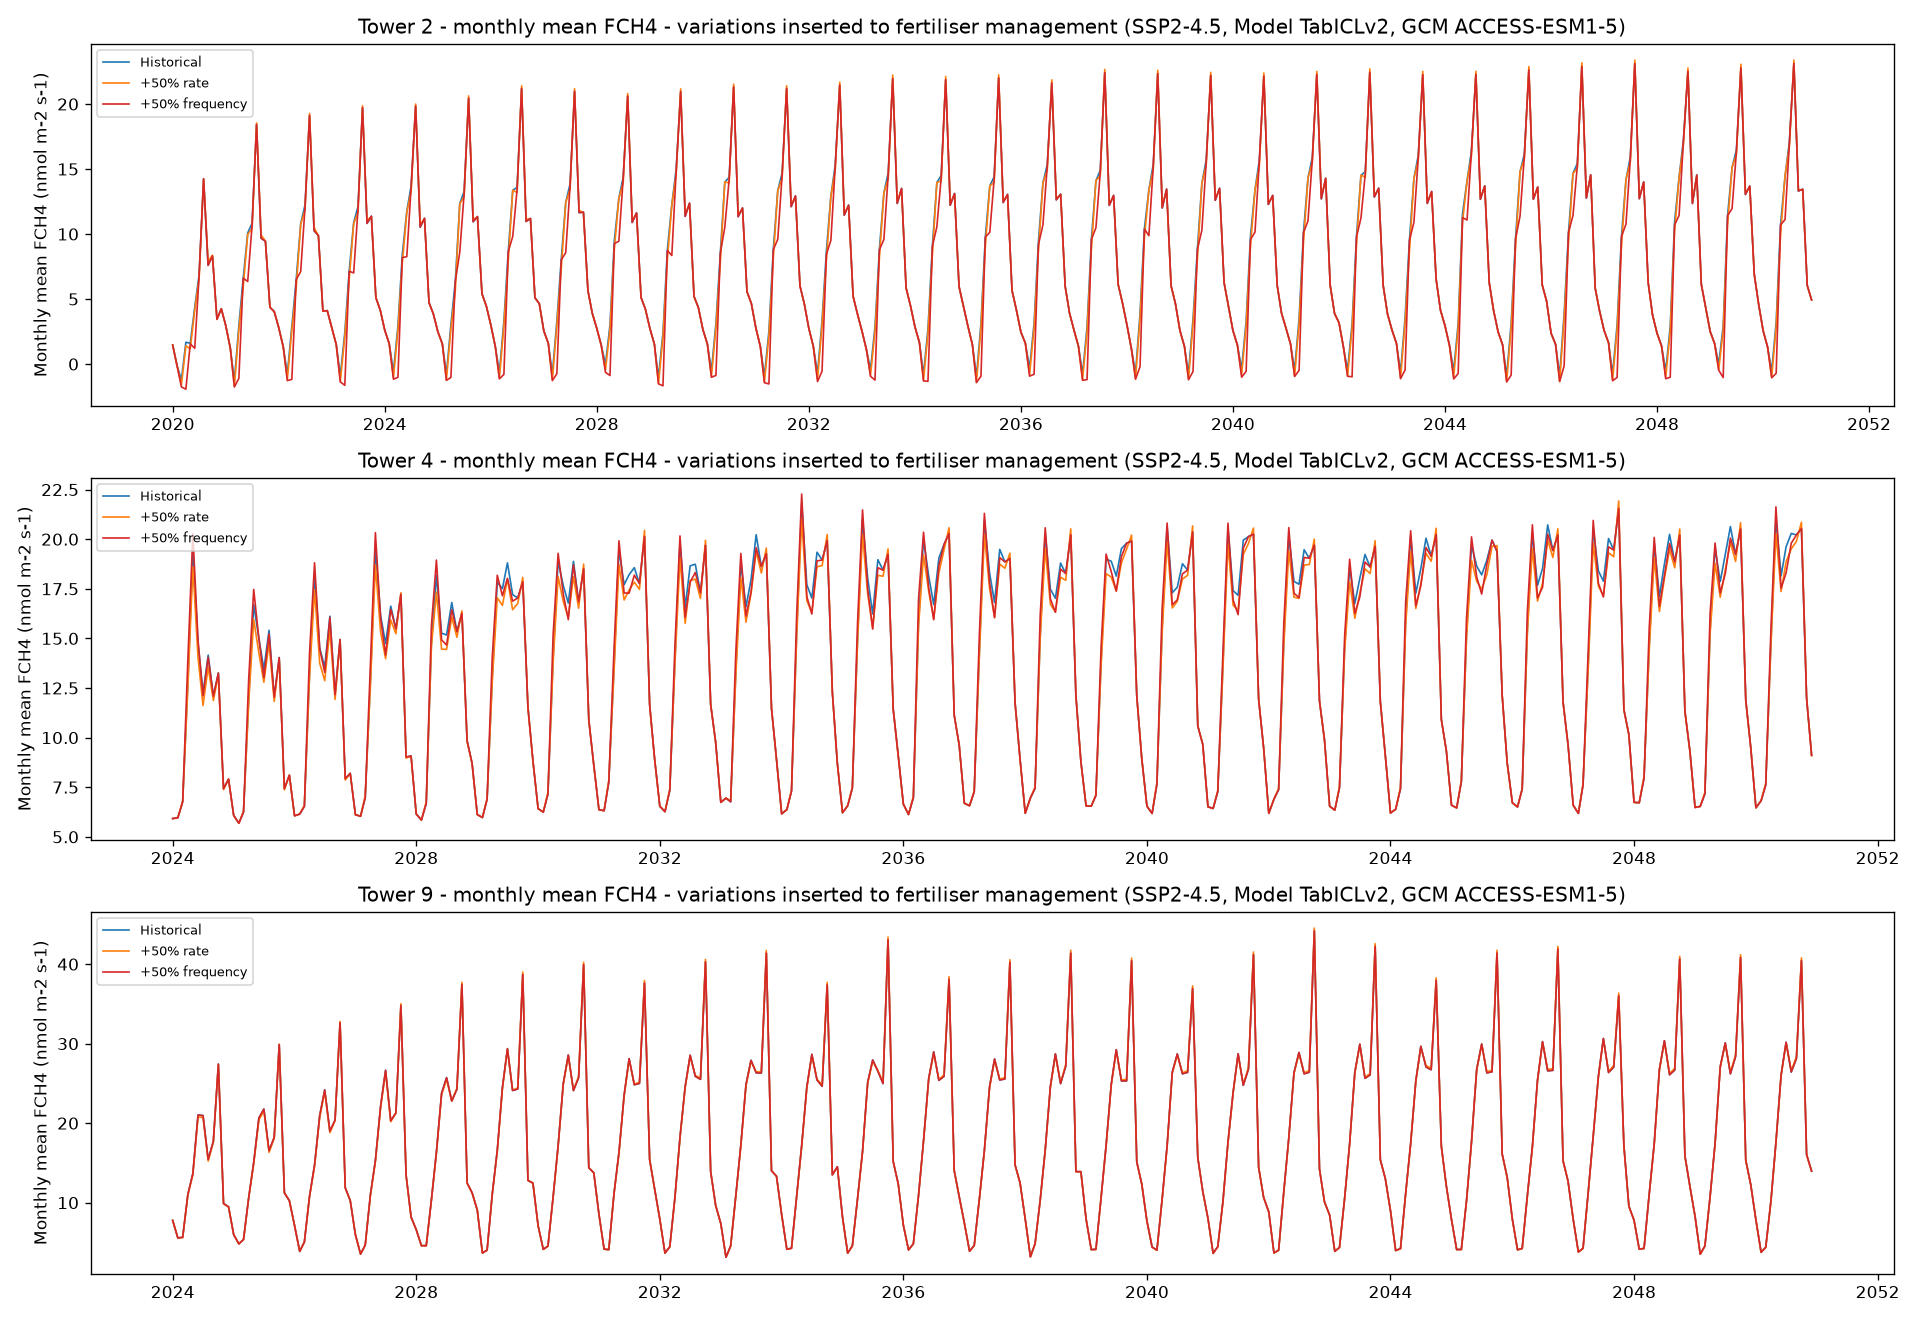
\includegraphics[width=\textwidth]{Figures/ch6_fertilizer_trajectory_ssp245.png}
\caption{
    Monthly mean FCH\textsubscript{4} (nmol~m\textsuperscript{-2}~s\textsuperscript{-1}) 
    at T2, T4 and T9 under SSP2-4.5 for the historical fertiliser-management baseline and its
$+50\%$-rate and $+50\%$-frequency perturbations, for a single illustrative trajectory
(restricted model, GCM ACCESS-ESM1-5, realisation~1). The three lines are visually near-identical
at every tower, consistent with Table~\ref{tab:management_scenario_results}'s finding that
fertiliser interventions produce only a small effect on predicted FCH\textsubscript{4}.
}
\label{fig:app_sp_fertilizer_trajectory_ssp245}
\end{figure}

\begin{figure}[htbp]
\centering
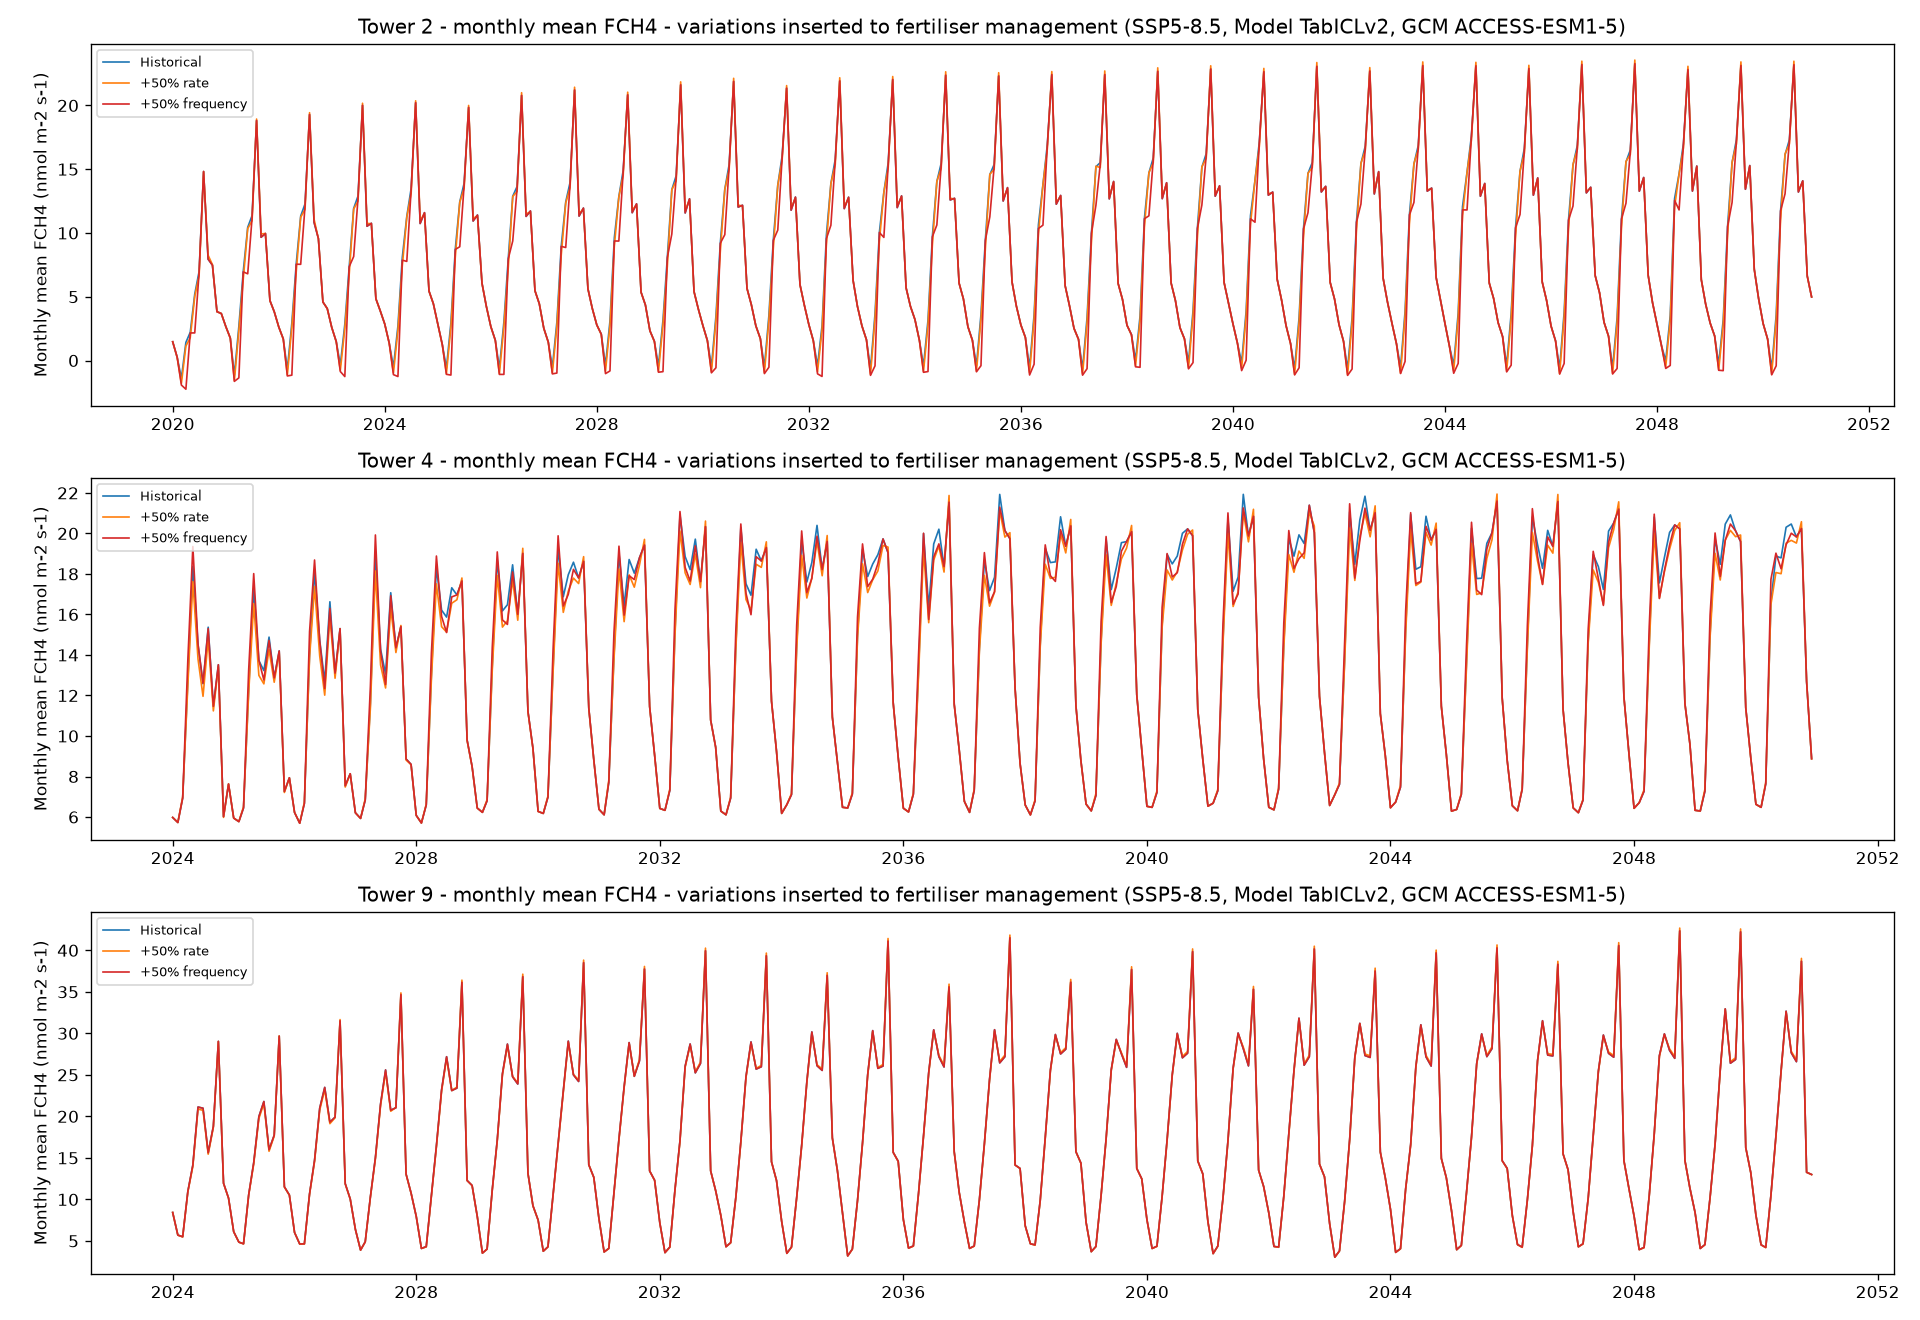
\includegraphics[width=\textwidth]{Figures/ch6_fertilizer_trajectory_ssp585.png}
\caption{
    Monthly mean FCH\textsubscript{4} (nmol~m\textsuperscript{-2}~s\textsuperscript{-1}) 
    at T2, T4 and T9 under SSP5-8.5 for the historical fertiliser-management baseline and its
$+50\%$-rate and $+50\%$-frequency perturbations, for a single illustrative trajectory
(restricted model, GCM ACCESS-ESM1-5, realisation~1). The three lines are visually near-identical
at every tower, consistent with Table~\ref{tab:management_scenario_results}'s finding that
fertiliser interventions produce only a small effect on predicted FCH\textsubscript{4}.
}
\label{fig:app_sp_fertilizer_trajectory_ssp585}
\end{figure}

\FloatBarrier

\chapter{Source Code}
\label{app:source-code}
\label{System Requirements}

Source code for all of the methods implemented in Chapters
\ref{Chap3}--\ref{Chap6} can be found in the GitHub repository:
\newline
\url{https://github.com/nicholas-tobias-00/COMP0191-Dissertation}.


\end{appendices}
%%%%%%%%%%%%%%%%%%%%%%%%%%%%%%%%%%%%%%%%%%%%%%%%%%%%%%%%%%%%%%%%%%%%%%%%%%%%%%%%
% GLOSSARY
% \clearpage
% \printglossaries

% INDEX?

\end{document}
